% =============================================================================
% Section 2: Problem formulation
% Intended to be \input{} into manuscript/main.tex, which already declares
% \section{Problem formulation} \label{sec:formulation} as a stub. Replace that
% stub with % =============================================================================
% Section 2: Problem formulation
% Intended to be \input{} into manuscript/main.tex, which already declares
% \section{Problem formulation} \label{sec:formulation} as a stub. Replace that
% stub with % =============================================================================
% Section 2: Problem formulation
% Intended to be \input{} into manuscript/main.tex, which already declares
% \section{Problem formulation} \label{sec:formulation} as a stub. Replace that
% stub with % =============================================================================
% Section 2: Problem formulation
% Intended to be \input{} into manuscript/main.tex, which already declares
% \section{Problem formulation} \label{sec:formulation} as a stub. Replace that
% stub with \input{sections/problem_formulation}.
%
% PACKAGES REQUIRED IN main.tex PREAMBLE (not currently present):
%   \usepackage{booktabs}
%   \usepackage{array}      (for the >{\raggedright\arraybackslash}p{} column type)
% =============================================================================

\section{Problem formulation}
\label{sec:formulation}

\subsection{Base geometry}
\label{sec:geometry}

The model geometry is the 1U immersion server of Muneeshwaran et al.~\cite{muneeshwaran2023}:
a copper plate-fin heat sink clamped to a four-die thermal test vehicle on a printed circuit
board, with a bank of non-dissipating memory modules alongside it, the whole tray submerged in a
sealed 1U tank. Coolant enters through a port on the tank floor directly beneath the heat sink
and leaves through two ports at the top of the opposite faces, the arrangement those authors call
the T-configuration. That choice of base is not a matter of taste. It is the only 1U immersion
architecture in the surveyed literature whose server tray, heat sink, tank, memory bank and mock
processor all carry printed dimension callouts, so the domain can be rebuilt without scaling
anything off a figure. It is also the architecture that Chun et al.~\cite{chun2026} identify as
prior bypass-control work, that B. Zhang et al.~\cite{zhang2026} state they reconstructed as their
own computational domain, that Khoshvaght-Aliabadi and co-workers rebuilt twice as a validation
replica~\cite{khoshvaghtaliabadi2026oblique,khoshvaghtaliabadi2026component}, and from which Kim
et al.~\cite{kim2025} took their inlet and outlet arrangement. Only the first of those four is a
reuse of the architecture as a study domain; the others are weaker forms of reliance and are
described here as such.

The bypass mechanism this paper is about is present in the base paper and was measured there.
Muneeshwaran et al.~\cite{muneeshwaran2023} swept the clearance between the heat sink and the 1U
tank inner wall at 5, 2 and 0~mm, reported a 3\% to 7.4\% rise in thermal resistance and a
0.7~$^{\circ}$C to 1.5~$^{\circ}$C rise in case temperature as the gap opened, and adopted the
no-gap build for everything that followed. Their flow visualisation shows the reason: fluid takes
the clearance because its hydraulic resistance is lower, and that stream does no useful heat
transfer. The open ratio of Section~\ref{sec:openratio} is the dimensionless generalisation of
exactly this clearance.

\begin{figure}[htbp]
\centering
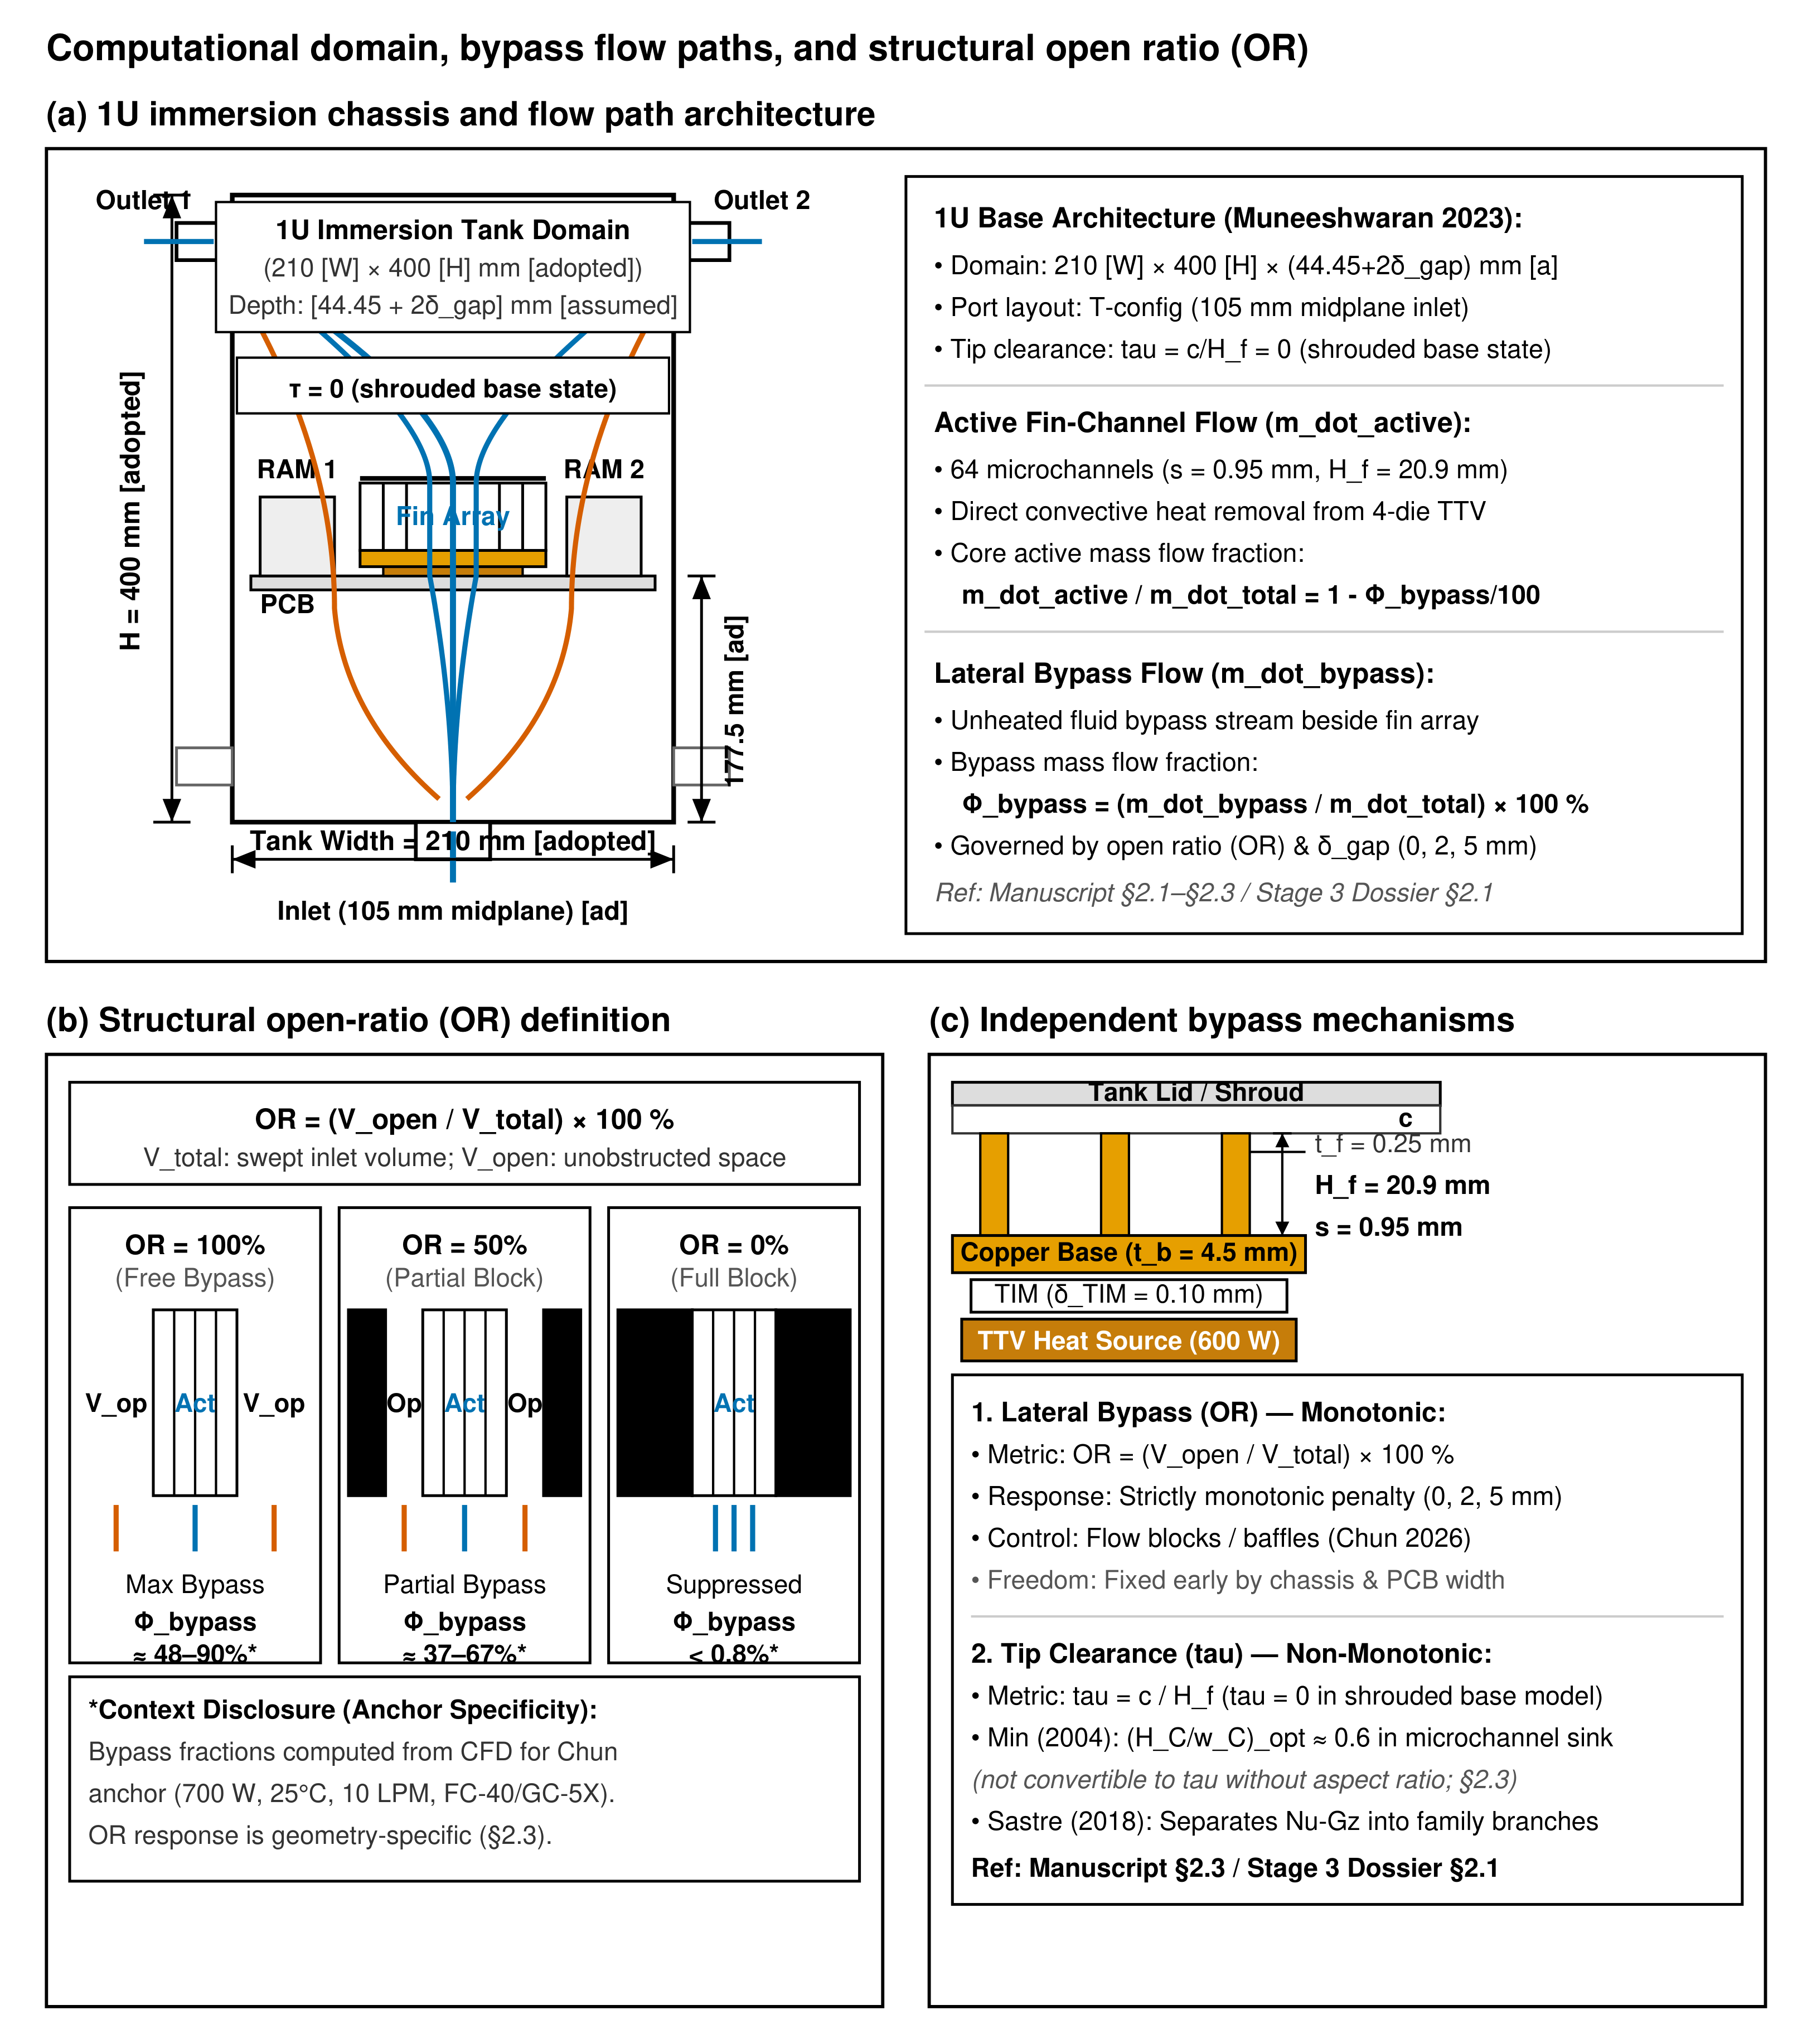
\includegraphics[width=\textwidth]{../figures/fig1_domain.png}
\caption{Computational domain, bypass flow paths and the open-ratio definition. (a) the 1U
immersion chassis with the active fin-channel flow and lateral bypass stream (with the shrouded
$\tau=0$ base state and independent tip clearance treated in panel (c)). (b) the open-ratio
definition at the heat-sink inlet plane across three blockage states. (c) lateral bypass and tip
clearance shown as the two independent mechanisms carried separately in this model, per
Section~\ref{sec:openratio}.}
\label{fig:domain}
\end{figure}

Table~\ref{tab:ledger-base} is the complete dimension ledger for the base model. Every row carries
one of three tags. A row tagged \texttt{[adopted]} is printed in the cited source at the cited
page, in body text, in a table, or as a dimension callout drawn on a figure. A row tagged
\texttt{[derived]} is computed from \texttt{[adopted]} rows, with the arithmetic shown. A row
tagged \texttt{[assumed]} is not available in any source consulted, and its value, its bounds and
the results it can move are stated in Section~\ref{sec:assumptions}. No row in the ledger is
digitised from a plot. Several of the \texttt{[adopted]} rows are recoverable only by rendering
the source page to an image and reading the drawing, because plain text extraction drops
dimension callouts that exist as vector labels inside a figure; those rows name the figure.

\begingroup
\footnotesize
\setlength{\tabcolsep}{4pt}
\begin{longtable}{@{}r>{\raggedright\arraybackslash}p{0.200\textwidth}c>{\raggedright\arraybackslash}p{0.135\textwidth}l>{\raggedright\arraybackslash}p{0.275\textwidth}@{}}
\caption{Dimension ledger for the base model, the 1U immersion server of Muneeshwaran et
al.~\cite{muneeshwaran2023}. Page numbers are the printed journal page of
\textit{Int.\ Commun.\ Heat Mass Transf.} \textbf{145} (2023) 106843, which coincides with the
PDF page index for this article.}
\label{tab:ledger-base}\\
\toprule
\# & Quantity & Symbol & Value & Tag & Source or arithmetic \\
\midrule
\endfirsthead
\multicolumn{6}{@{}l}{\normalfont\itshape Table~\ref{tab:ledger-base} continued}\\
\toprule
\# & Quantity & Symbol & Value & Tag & Source or arithmetic \\
\midrule
\endhead
\midrule
\multicolumn{6}{@{}r}{\normalfont\itshape continued on next page}\\
\endfoot
\bottomrule
\endlastfoot
1  & Rack unit height, server slot        &            & 44.45~mm & \texttt{[adopted]} & p.~1, abstract \\
2  & Heat-sink base thickness             & $t_b$      & 4.5~mm   & \texttt{[adopted]} & p.~3, \S2.1 \\
3  & Fin thickness                        & $t_f$      & 0.25~mm  & \texttt{[adopted]} & p.~3, \S2.1 \\
4  & Fin height                           & $H_f$      & 20.9~mm  & \texttt{[adopted]} & p.~3, \S2.1 \\
5  & Fin pitch, two builds                & $p_f$      & 1.2 and 2.2~mm & \texttt{[adopted]} & p.~3; Table~3, p.~7 \\
6  & Fin channel width                    & $s$        & 0.95~mm; 1.95~mm & \texttt{[derived]} & $s=p_f-t_f$ \\
7  & Channel hydraulic diameter           & $D_h$      & 1.817~mm; 3.567~mm & \texttt{[derived]} & $D_h=2sH_f/(s+H_f)$ \\
8  & Heat-sink stack height               & $t_b+H_f$  & 25.4~mm  & \texttt{[derived]} & $4.5+20.9$ \\
9  & Heat-sink base footprint             & $L\times W$& 118~mm $\times$ 78~mm & \texttt{[adopted]} & Fig.~2(b), p.~5, rendered callouts \\
10 & Raised finned-section callouts       &            & 81~mm and 31.2~mm & \texttt{[adopted]} & Fig.~2(b), p.~5. The drawing does not label which feature each callout terminates on \\
11 & Fin-bank plan area                   & $A_{bank}$ & 78~mm $\times$ 118~mm & \texttt{[assumed]} & Bounds 31.2 $\times$ 81~mm to 78 $\times$ 118~mm; see Section~\ref{sec:assumptions} \\
12 & Fin count, $p_f=1.2$~mm              & $N_f$      & 65 fins, 64 channels & \texttt{[derived]} & $Nt_f+(N-1)s=W$ on row 11 \\
13 & Fin count, $p_f=2.2$~mm              & $N_f$      & 36 fins, 35 channels & \texttt{[derived]} & same relation on row 11 \\
14 & Channel free-flow area, base build   & $A_c$      & $1.271\times10^{-3}$~m$^2$ & \texttt{[derived]} & $64\times0.95\times20.9$~mm$^2$ \\
15 & Heat-sink material                   &            & copper   & \texttt{[adopted]} & p.~3, \S2.1 \\
16 & Mock CPU package footprint           &            & 48~mm $\times$ 68~mm & \texttt{[adopted]} & Fig.~2(e), p.~7, rendered callouts \\
17 & Die count                            &            & 4, independently modulated & \texttt{[adopted]} & p.~3, \S2.1; Fig.~2(e), p.~7 \\
18 & Individual die footprint             &            & 2 $\times$ 2 tiling of a centred block & \texttt{[assumed]} & Bounds 50\% to 90\% of the package footprint; see Section~\ref{sec:assumptions} \\
19 & Thermal interface material           &            & grease TC-5888, $k=5.2$ &  \texttt{[adopted]} & p.~3, \S2.1; $k$ in W~m$^{-1}$~K$^{-1}$ \\
20 & TIM bond-line thickness              & $\delta_{TIM}$ & 0.10~mm & \texttt{[assumed]} & Bounds 0.05 to 0.20~mm; see Section~\ref{sec:assumptions} \\
21 & Bypass gap, heat sink to tank wall   & $\delta_{gap}$ & 0, 2, 5~mm & \texttt{[adopted]} & p.~5, \S3.2; Fig.~6, p.~9; Fig.~7, p.~10 \\
22 & Tank, long horizontal dimension      &            & 210~mm   & \texttt{[adopted]} & Fig.~2(c), p.~6, rendered callouts \\
23 & Tank, vertical dimension             &            & 400~mm   & \texttt{[adopted]} & Fig.~2(c), p.~6 \\
24 & Bottom inlet axis from tank end wall &            & 105~mm   & \texttt{[adopted]} & Fig.~2(c), p.~6; $105=210/2$, so the inlet is on the tank mid-plane \\
25 & Side port axes from floor and ceiling&            & 27.5~mm  & \texttt{[adopted]} & Fig.~2(c), p.~6 \\
26 & Heat-sink underside above tank floor &            & 177.5~mm & \texttt{[adopted]} & Fig.~2(c), p.~6 \\
27 & Tank depth, out-of-plane             &            & 44.45~mm internal $+\,2\delta_{gap}$ & \texttt{[assumed]} & Bounds 44.45 to 55~mm internal; see Section~\ref{sec:assumptions} \\
28 & Tank wall material                   &            & acrylic, adiabatic outer face & \texttt{[assumed]} & $k=0.19$; bounds 0.19 to 16.4~W~m$^{-1}$~K$^{-1}$; see Section~\ref{sec:assumptions} \\
29 & Server tray outline                  &            & 275 and 245~mm; 201 and 141.7~mm & \texttt{[adopted]} & Fig.~2(a), p.~5, rendered callouts \\
30 & Memory bank envelope                 &            & 149 $\times$ 59.3 $\times$ 34.1~mm; pitch 7.5~mm; gap 3.3~mm & \texttt{[adopted]} & Fig.~2(d), p.~6, rendered callouts \\
31 & Memory thermal load                  &            & zero, flow obstruction only & \texttt{[adopted]} & p.~3, \S2.1 \\
32 & PCB thickness                        &            & 2.4~mm   & \texttt{[assumed]} & From Khoshvaght-Aliabadi et al.~\cite{khoshvaghtaliabadi2026oblique}, Table~1, p.~5; bounds 1.6 to 3.0~mm \\
\end{longtable}
\endgroup

\begin{figure}[htbp]
\centering
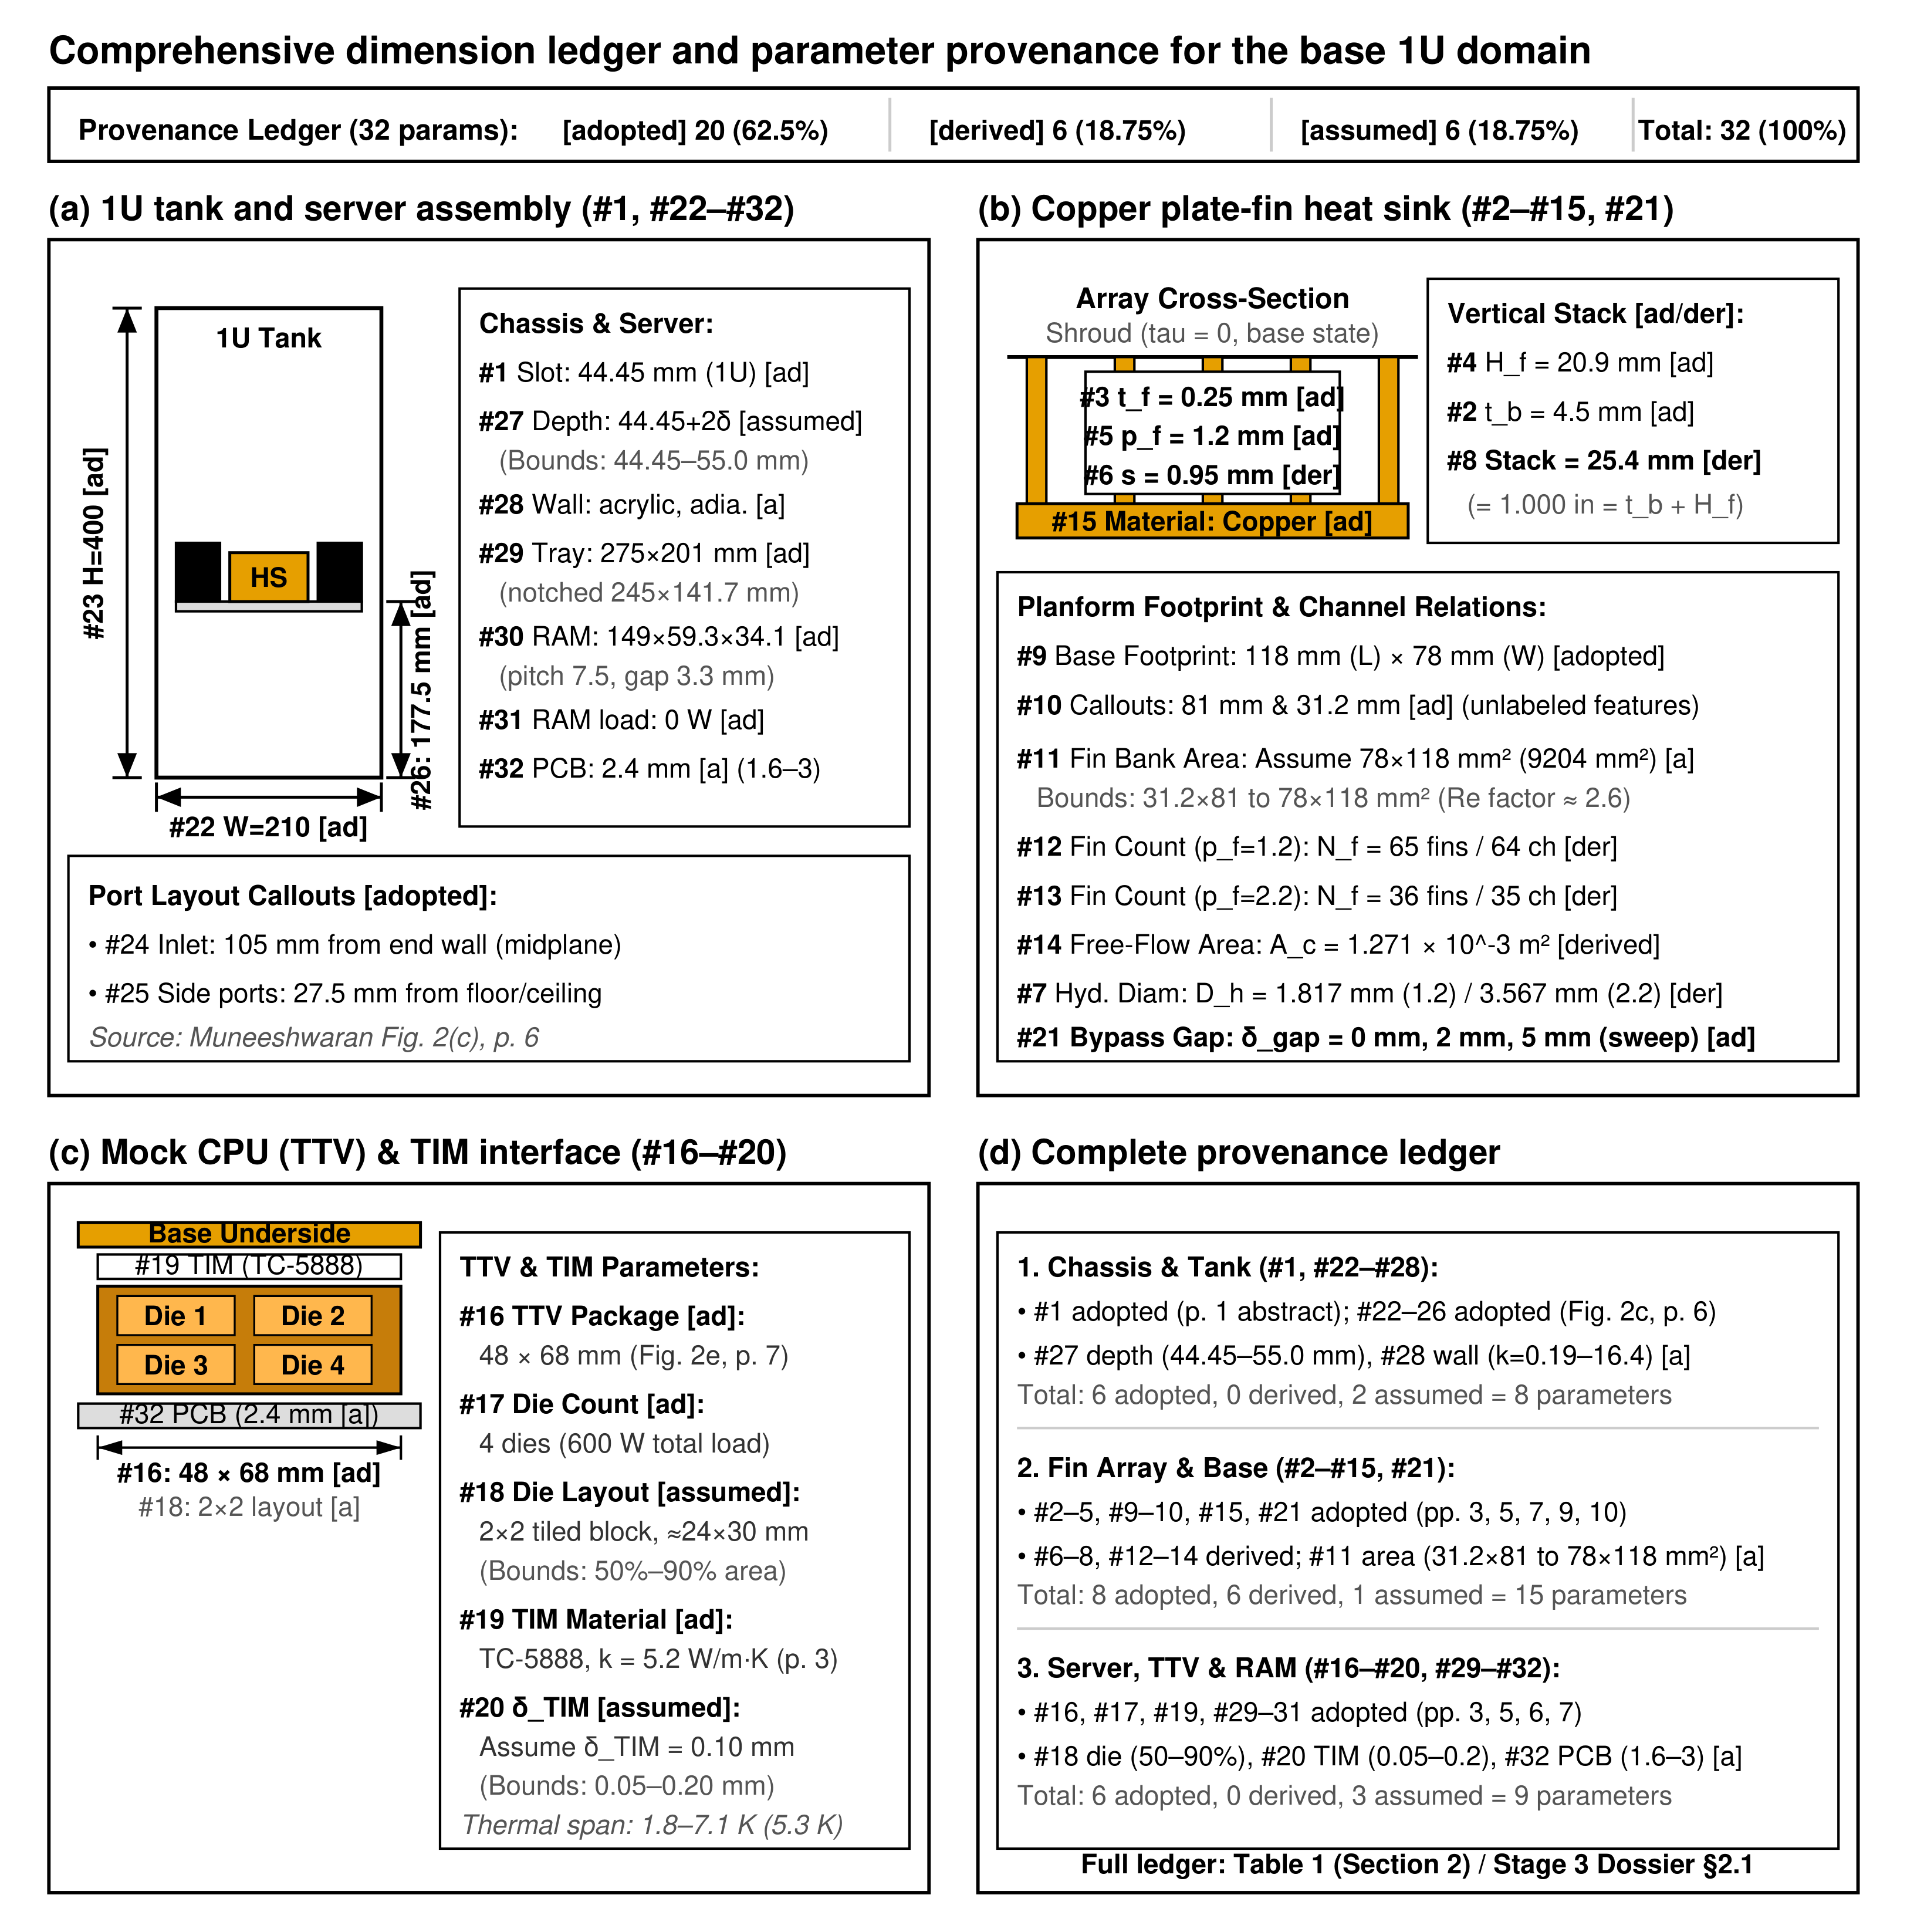
\includegraphics[width=\textwidth]{../figures/fig2_dimension_ledger.png}
\caption{Dimension ledger and parameter provenance for the base model geometry, matching
Table~\ref{tab:ledger-base}. Adopted, derived and assumed dimensions are visually distinguished
so that the source of every number in the model is visible at a glance.}
\label{fig:ledger}
\end{figure}

Two conventions follow from the ledger and are stated here so that no downstream quantity is
ambiguous. First, the fin bank is taken to span the 78~mm base width, so the span sets the channel
count and the 118~mm base length is the channel flow length. Second, the channel hydraulic
diameter of row 7 is the length scale for every Reynolds and Nusselt number reported in this
paper. That second point needs saying because the bypass and tip-clearance literature this work
builds on does not share a convention: Sastre et al.~\cite{sastre2018} use the hydraulic diameter
of the finned cross-section including the clearance slab, Mei et al.~\cite{mei2014} use the pin
diameter with the maximum velocity, Jeng~\cite{jeng2008} uses the bare rectangular duct with the
inlet velocity, Shahsavar et al.~\cite{shahsavar2021} use four times the array volume over its
wetted area, Shrigondekar et al.~\cite{shrigondekar2023} use the bare fin spacing, and Min et
al.~\cite{min2004} report no Reynolds number at all and sweep pumping power instead. Five
incompatible length scales across six papers is a large part of why no dimensionless framework for
this problem exists yet, and every literature value quoted in this paper is recomputed on the
convention above before it is compared with anything.

Applying that convention to the base geometry gives a channel Reynolds number
$\mathrm{Re}_{ch}=\dot{m}D_h/(A_c\mu)$ of roughly 5 to 122 over the 1 to 3~LPM flow range and the
15 to 35~$^{\circ}$C inlet range, if all flow is forced through the fins. The band is wide, and it
is wide for an honest reason: it carries the factor of about 2.6 between the two bounds of the
fin-bank span in row 11. No single-valued channel Reynolds number is quoted for the base geometry
anywhere in this paper. The one directly printed check available is Shrigondekar et
al.~\cite{shrigondekar2023}, who report a fin-spacing Reynolds number of about 10 to 70 for FC-40
on the same rig at the same flow rates and the same two fin pitches. Converted onto the fin-spacing
length scale, the wide-span bound of row 11 gives 2.5 to 46 and the narrow-span bound gives 6.4 to
114. The printed value therefore sits inside the narrow band and partly above the wide one, which
means this check leans against the value adopted rather than confirming it. That is recorded here
rather than smoothed over.

\subsection{Reference configuration for the anchor comparison}
\label{sec:v3}

A second, fully dimensioned geometry is carried alongside the base model so that the open-ratio
results of Chun et al.~\cite{chun2026} can be reproduced without rescaling anything.
Table~\ref{tab:ledger-v3} is its ledger. It is not a substitute for the base model and no result
from the two configurations is pooled.

\begingroup
\footnotesize
\setlength{\tabcolsep}{4pt}
\begin{longtable}{@{}l>{\raggedright\arraybackslash}p{0.225\textwidth}>{\raggedright\arraybackslash}p{0.185\textwidth}l>{\raggedright\arraybackslash}p{0.245\textwidth}@{}}
\caption{Dimension ledger for the reference configuration used in the anchor comparison, the 1U
plate-fin build of Chun et al.~\cite{chun2026}. Page numbers are the printed journal page of
\textit{Energy} \textbf{361} (2026) 141967.}
\label{tab:ledger-v3}\\
\toprule
\# & Quantity & Value & Tag & Source or arithmetic \\
\midrule
\endfirsthead
\multicolumn{5}{@{}l}{\normalfont\itshape Table~\ref{tab:ledger-v3} continued}\\
\toprule
\# & Quantity & Value & Tag & Source or arithmetic \\
\midrule
\endhead
\midrule
\multicolumn{5}{@{}r}{\normalfont\itshape continued on next page}\\
\endfoot
\bottomrule
\endlastfoot
A1  & 1U internal slot spacing        & 44.45~mm & \texttt{[adopted]} & p.~5, \S2.1 \\
A2  & Fin thickness                   & 2~mm     & \texttt{[adopted]} & Fig.~2(a), p.~5, callout under a ``Unit : mm'' header \\
A3  & Fin spacing                     & 3~mm     & \texttt{[adopted]} & Fig.~2(a), p.~5 \\
A4  & Fin height                      & 20~mm    & \texttt{[adopted]} & Fig.~2(a), p.~5 \\
A5  & Fin pitch                       & 5~mm     & \texttt{[derived]} & $2+3$ \\
A6  & Heat-sink base plate            & 72~mm width $\times$ 106~mm flow length & \texttt{[adopted]} & Fig.~2(a), p.~5 \\
A7  & Fin count                       & 15 fins, 14 channels & \texttt{[derived]} & $2N+3(N-1)=72$ gives $N=15$ exactly \\
A8  & Channel free-flow area          & $8.40\times10^{-4}$~m$^2$ & \texttt{[derived]} & $14\times3\times20$~mm$^2$ \\
A9  & Channel hydraulic diameter      & 5.217~mm & \texttt{[derived]} & $2(3)(20)/23$ \\
A10 & Copper block, mock CPU          & 50 $\times$ 65 $\times$ 8~mm & \texttt{[adopted]} & Fig.~2(a), p.~5 \\
A11 & TIM, indium foil thickness      & $\approx$0.1~mm & \texttt{[adopted]} & p.~6, \S2.1 \\
A12 & Heat-sink centre spacing on PCB & 60~mm    & \texttt{[adopted]} & p.~6, \S2.1, and Fig.~2(a), p.~5 \\
A13 & Tank internal width             & 423~mm   & \texttt{[adopted]} & Fig.~2(a), p.~5, right-hand panel headed ``Immersion tank'' \\
A14 & Tank internal height, outlet plane to distribution-plate plane & 430~mm & \texttt{[adopted]} & Fig.~2(a), p.~5, right-hand panel \\
A15 & Distribution plate, 1U build    & 10 holes, 10~mm diameter & \texttt{[adopted]} & p.~5, \S2.1 \\
A16 & Distribution plate, 3U build    & 30 holes, 5~mm diameter & \texttt{[adopted]} & p.~5, \S2.1 \\
A17 & Tank material                   & SUS304, double-layer insulation, tempered-glass window & \texttt{[adopted]} & p.~4, \S2.1; properties Table~2, p.~6 \\
A18 & Flow-control block material     & acrylic  & \texttt{[adopted]} & p.~6, \S2.1 \\
A19 & Flow-control block dimensions   & not dimensioned in the source & \texttt{[assumed]} & The open ratio is therefore defined here by the volume a block occludes, never by a block dimension \\
A20 & Tank external envelope          & not printed in the source & \texttt{[assumed]} & Not required: the computational domain is the wetted interior bounded by A13, A14 and A1 \\
A21 & Metal-foam alternative core     & 10~PPI, porosity 0.9; sweep 5 to 15~PPI, porosity 0.5 to 0.9 & \texttt{[adopted]} & p.~15 and p.~18, \S3.3 \\
\end{longtable}
\endgroup

Three specific gaps in this reference configuration are carried openly rather than closed
silently, because an independent reproducibility check found them and they are real. The source
does not print the tank's third, out-of-plane dimension, does not print the heat-sink base
thickness, and does not give the numerical inlet profile, outlet type or tank-wall thermal
condition, so the anchor comparison in Section~\ref{sec:verification} is a best-effort check
against a paper that does not fully close its own specification, not a fully reproducible
benchmark. The same three gaps are the reason A19, A20 and the base thickness never enter a
reported quantity.

\subsection{Open ratio}
\label{sec:openratio}

The bypass metric is adopted verbatim from Chun et al.~\cite{chun2026}, who introduce it as an
unnumbered display equation on their p.~11 and illustrate it in their Fig.~8. Their words for it,
quoted so that nothing is quietly reinterpreted here, are that the open ratio is
\textit{the volumetric fraction of the unobstructed fluid inlet space relative to the total heat
sink inlet volume}:

\begin{equation}
\mathrm{OR} = \frac{V_{\mathrm{open}}}{V_{\mathrm{total}}}\times 100 \quad (\%)
\label{eq:or}
\end{equation}

\noindent
Named for the geometry of Table~\ref{tab:ledger-base}, the two volumes in Eq.~(\ref{eq:or}) are
the following. $V_{\mathrm{total}}$ is the total heat-sink inlet volume, the fluid volume swept
out by the heat-sink inlet plane over the inlet-plane thickness, that is the plan area of the 1U
slot facing the heat sink multiplied by the inlet-plane thickness, spanning the full tank width
available to the flow at that height. $V_{\mathrm{open}}$ is the unobstructed fluid inlet space,
the part of $V_{\mathrm{total}}$ occupied by neither the heat sink nor a flow-control block, that
is the volume through which fluid can reach the outlets without passing between the fins. At
$\mathrm{OR}=100\%$ the tank is unobstructed and bypass is free. At $\mathrm{OR}=0\%$ every
entering parcel is directed through the heat-source region.

Three properties of the definition travel with it, because dropping any of them changes what the
number means. It is a volume ratio at the inlet plane, not an area ratio and not a clearance in
millimetres; the source never converts it to a gap width. It is geometry-specific, and the source
says so, so any open ratio quoted here travels with the geometry it was measured on. And the
blocking acts laterally, from both edges symmetrically, which in the 1U build means the top gap is
absent and the open ratio is a purely lateral quantity.

Open ratio is a geometric input. Its companion output, also taken from
Chun et al.~\cite{chun2026}, is the bypass mass fraction,

\begin{equation}
\dot{m}_{\mathrm{bypass}} = \dot{m}_{\mathrm{total}} - \dot{m}_{\mathrm{active}},
\qquad
\Phi_{\mathrm{bypass}} = \frac{\dot{m}_{\mathrm{bypass}}}{\dot{m}_{\mathrm{total}}}\times 100
\quad (\%),
\label{eq:phibypass}
\end{equation}

\noindent
where the bypass region is the flow region excluding the heat-sink passages and the region
directed toward the heat source. This paper reports $\mathrm{OR}$ as the design variable and
$\Phi_{\mathrm{bypass}}$ as the computed response, in the same pairing the source uses.

Lateral bypass and tip clearance are carried as two separate parameters and are never combined
into one scalar. The tip clearance ratio is defined as

\begin{equation}
\tau = \frac{c}{H_f},
\label{eq:tau}
\end{equation}

\noindent
the clearance height over the fin height, and is held at $\tau=0$ in the base configuration. Four
reasons keep the two apart. The 1U build that defines the open ratio has already eliminated the
top gap, so folding a tip term into it would redefine the source's own quantity while keeping its
name. No study surveyed here varies both mechanisms; every tip-clearance study varies only the tip
gap and both side-bypass studies vary only the side gap, so a combined ratio would be a quantity
with no supporting measurement anywhere. Jeng~\cite{jeng2008} argues the point directly, noting
that the tip gap dominates in magnitude and can be changed late in a design while the channel
width is fixed early by the board width, which in a 1U immersion chassis holds with extra force.
And the two responses have different shapes. Tip clearance is non-monotonic and has an interior
optimum: Min et al.~\cite{min2004} report a minimum thermal resistance of 0.058~$^{\circ}$C~W$^{-1}$
at a clearance-to-channel-width ratio of 0.6 under 2.27~W of pumping power, and Mei et
al.~\cite{mei2014} report the same competing-effects reversal. Lateral bypass is monotonic and
always detrimental, in Muneeshwaran et al.~\cite{muneeshwaran2023} across the 0 to 5~mm gap sweep
and in Chun et al.~\cite{chun2026} across the open-ratio sweep. Collapsing a bounded parameter
with an optimum and a monotone detrimental one into a single scalar would make any interior
optimum in the combined ratio unattributable to either mechanism. Sastre et al.~\cite{sastre2018}
supply the warning empirically: even one clearance parameter was strong enough to split their
Nusselt-Graetz curves into separate families rather than one fit.

One out-of-sample check on the open ratio exists and is used. Jeng~\cite{jeng2008} parameterises
lateral bypass around a square pin-fin sink as the ratio $W/L$ of channel width to sink length. For
a constant-height inlet plane the two parameterisations map exactly, $\mathrm{OR} = (1-L/W)\times
100$, so $W/L$ of 1, 2, 3 and 5 correspond to open ratios of 0, 50, 66.7 and 80\%. Jeng's
recommendation of $W/L$ between 2 and 3 therefore sits inside the range swept here, in a different
fluid and a different fin type. The mapping is derived here, not printed in either source, and it
holds only when the open volume is the lateral space at the same inlet-plane height.

\subsection{Working fluids and thermophysical properties}
\label{sec:properties}

Two dielectric coolants are used. FC-40, a perfluorinated fluorocarbon, is the primary fluid: it is
the one coolant for which more than one independent group in this literature has published usable
property data, so a property error can be caught by cross-checking rather than trusted. GC-5X, an
oil-based dielectric, is the high-viscosity contrast case. Carrying two fluids is not decoration.
Chun et al.~\cite{chun2026} show that open-ratio sensitivity is a strong function of viscosity,
with thermal resistance falling 6.1\% for FC-40 but 45.6\% for GC-5X as the bypass is closed, so a
framework claimed to be dimensionless must be exercised across more than one Prandtl decade or the
claim is untested.

Table~\ref{tab:fluidprops} gives the property treatment and the source of every value.

\begin{table}[htbp]
\centering
\caption{Coolant thermophysical properties and their sources. The correlations of Chun et
al.~\cite{chun2026} take $T$ in kelvin; see the discussion below.}
\label{tab:fluidprops}
\footnotesize
\setlength{\tabcolsep}{4pt}
\begin{tabular}{@{}l>{\raggedright\arraybackslash}p{0.105\textwidth}>{\raggedright\arraybackslash}p{0.405\textwidth}>{\raggedright\arraybackslash}p{0.215\textwidth}@{}}
\toprule
Fluid & Property & Value or correlation ($T$ in K) & Source \\
\midrule
FC-40 & $\rho$    & $2499 - 2.16\,T$~kg~m$^{-3}$ & \cite{chun2026}, Table~3, p.~7 \\
FC-40 & $k$       & $0.086 - 6.90\times10^{-5}\,T$~W~m$^{-1}$~K$^{-1}$ & \cite{chun2026}, Table~3, p.~7 \\
FC-40 & $c_p$     & $590 + 1.55\,T$~J~kg$^{-1}$~K$^{-1}$ & \cite{chun2026}, Table~3, p.~7 \\
FC-40 & $\mu$     & $0.0429 - 0.162\times10^{-3}\,T$ $+\;1.08\times10^{-7}\,T^2$~Pa~s & \cite{chun2026}, Table~3, p.~7 \\
FC-40 & $\rho$ & 1874.44~kg~m$^{-3}$ at 16~$^{\circ}$C & \cite{muneeshwaran2023}, Table~4, p.~7 \\
FC-40 & $\nu$ & $5\times10^{-6}$, $1.5\times10^{-6}$, $5.4\times10^{-7}$~m$^2$~s$^{-1}$ at 0, 40, 100~$^{\circ}$C & \cite{muneeshwaran2023}, Table~4, p.~7 \\
FC-40 & $c_p$ & 1014, 1076, 1169.4~J~kg$^{-1}$~K$^{-1}$ at 0, 40, 100~$^{\circ}$C & \cite{muneeshwaran2023}, Table~4, p.~7 \\
FC-40 & $k$ & 0.067, 0.0642, 0.0601~W~m$^{-1}$~K$^{-1}$ at 0, 40, 100~$^{\circ}$C & \cite{muneeshwaran2023}, Table~4, p.~7 \\
FC-40 & $\beta$   & $1.2\times10^{-3}$~K$^{-1}$ & \cite{muneeshwaran2023}, Table~4, p.~7 \\
FC-40 & Boiling pt. & 165~$^{\circ}$C at 1~bar & \cite{muneeshwaran2023}, Table~4, p.~7 \\
FC-40 & $\mathrm{Pr}$ & 67.5 at 25~$^{\circ}$C & \texttt{[derived]} from the correlations above \\
\midrule
GC-5X & $\rho$    & $1049.862 - 0.75\,T$~kg~m$^{-3}$ & \cite{chun2026}, Table~3, p.~7 \\
GC-5X & $k$       & $0.199367 - 1.8\times10^{-4}\,T$~W~m$^{-1}$~K$^{-1}$ & \cite{chun2026}, Table~3, p.~7 \\
GC-5X & $c_p$     & $2076.055 + 0.3\,T$~J~kg$^{-1}$~K$^{-1}$ & \cite{chun2026}, Table~3, p.~7 \\
GC-5X & $\mu$     & $0.6449 - 4.1234\times10^{-3}\,T$ $+\;8.9697\times10^{-6}\,T^2$ $-\;6.5833\times10^{-9}\,T^3$~Pa~s & \cite{chun2026}, Table~3, p.~7 \\
GC-5X & $\beta$   & $9.08\times10^{-4}$~K$^{-1}$ at 25~$^{\circ}$C & \texttt{[derived]}, $\beta=-\rho^{-1}\partial\rho/\partial T$ on the density fit of this table. No measured value is printed in any source consulted \\
GC-5X & $\mathrm{Pr}$ & 570 at 25~$^{\circ}$C & \texttt{[derived]} from the correlations above \\
\bottomrule
\end{tabular}
\end{table}

Two findings about these properties came out of checking them rather than copying them, and both
change how the correlations may be used.

The first is that the correlations of Chun et al.~\cite{chun2026} take $T$ in kelvin, which their
paper does not state and their own nomenclature contradicts by defining $T$ in degrees Celsius.
The evidence is arithmetic and it is decisive. With $T$ in kelvin the FC-40 density fit returns
1874.4~kg~m$^{-3}$ at 289.15~K, against the 1874.44~kg~m$^{-3}$ at 16~$^{\circ}$C measured
independently by Muneeshwaran et al.~\cite{muneeshwaran2023}. The conductivity fit returns 0.0672,
0.0644 and 0.0603~W~m$^{-1}$~K$^{-1}$ at 0, 40 and 100~$^{\circ}$C against their printed 0.067,
0.0642 and 0.0601, and the specific-heat fit returns 1013.4, 1075.4 and 1168.4~J~kg$^{-1}$~K$^{-1}$
against their printed 1014, 1076 and 1169.4. Three properties agree to better than 0.1\% at three
temperatures each on one unit convention and are irreconcilable on the other. The same conclusion
follows independently from the source's own mass-flow table, which converts to exactly 5.00~LPM per
heat sink at the stated 10~LPM for two heat sinks only when the density is evaluated in kelvin.
This is an inference from the paper's numbers, not a printed statement, and it should be confirmed
with the corresponding author before any anchor result is reproduced.

The second finding is a limit on the FC-40 viscosity fit, and it constrains the model. That
quadratic reaches zero at about 343~K, or 70~$^{\circ}$C, and is negative above it, so it cannot be
used at wall temperatures approaching the 80~$^{\circ}$C case-temperature limit of the base
paper~\cite{muneeshwaran2023}. Within its useful band it is good: against the kinematic-viscosity
points of Muneeshwaran et al.\ interpolated logarithmically it agrees to 1.2\% at 35~$^{\circ}$C
and 3.9\% at 25~$^{\circ}$C, degrading to 13\% at 15~$^{\circ}$C and 30\% at 0~$^{\circ}$C. FC-40
viscosity is therefore evaluated from the fit between 20 and 60~$^{\circ}$C and from the measured
points of Muneeshwaran et al.\ outside that band. The GC-5X cubic stays positive and monotone
across the whole range of interest and needs no such restriction.

Solid properties are listed in Table~\ref{tab:solidprops}. Where two sources print a value, both
are named, and where they agree exactly that is said, because agreement between independently
published tables is the only property check available in the absence of a measurement of our own.

\begin{table}[htbp]
\centering
\caption{Solid domain properties and their sources. Density in kg~m$^{-3}$, specific heat in J~kg$^{-1}$~K$^{-1}$, thermal conductivity in W~m$^{-1}$~K$^{-1}$.}
\label{tab:solidprops}
\footnotesize
\setlength{\tabcolsep}{4pt}
\begin{tabular}{@{}>{\raggedright\arraybackslash}p{0.155\textwidth}cc>{\raggedright\arraybackslash}p{0.105\textwidth}>{\raggedright\arraybackslash}p{0.30\textwidth}@{}}
\toprule
Domain & $\rho$ & $c_p$ & $k$ & Source \\
\midrule
Copper, fins and base & 8978 & 381 & 387.6 & \cite{chun2026}, Table~2, p.~6; the identical triplet is printed independently in \cite{khoshvaghtaliabadi2026oblique}, Table~1, p.~5 \\
TIM, base model, thermal grease & \multicolumn{2}{c}{not printed} & 5.2 & \cite{muneeshwaran2023}, p.~3, \S2.1 \\
TIM, reference configuration, indium & 7310 & 234 & 81.8 & \cite{chun2026}, Table~2, p.~6 \\
PCB substrate & 1850 & 1000 & 0.3 & \cite{khoshvaghtaliabadi2026oblique}, Table~1, p.~5 \\
PCB substrate, alternative & 3600 & 720 & 42.0 in-plane, 0.5 cross-plane & \cite{chun2026}, Table~2, p.~6 \\
SUS304, reference configuration tank & 8000 & 500 & 16.4 & \cite{chun2026}, Table~2, p.~6 \\
Acrylic, flow-control block and tank wall & 1180 & 1460 & 0.21 & \cite{chun2026}, Table~2, p.~6 \\
\bottomrule
\end{tabular}
\end{table}

The two PCB entries disagree by two orders of magnitude in conductivity because they describe
different things: one is an isotropic bulk laminate value, the other resolves the copper-plane
anisotropy. The isotropic entry is used for the base model, where the board is an unloaded
conduction path, and the anisotropic entry is used for the anchor comparison so that the
reference configuration keeps its own source's convention. Neither value moves a reported quantity
in this work, since the board carries no thermal load in the base model. All solid property values
in Table~\ref{tab:solidprops} are attributed within their source to further references rather than
measured there, and are carried on that basis.

\subsection{Assumptions}
\label{sec:assumptions}

Eight quantities in Tables~\ref{tab:ledger-base} and \ref{tab:ledger-v3} are not available in any
source consulted. Each is listed below with the value taken, the reason, the defensible bounds and
the results it can move. Nothing here is assumed because it was convenient, and nothing that a
result depends on is hidden inside a sentence.

\noindent\textbf{Fin-bank plan area, 78~mm $\times$ 118~mm (row 11).}\ The base outline of the heat sink is
dimensioned but the drawing does not label which feature its two interior callouts, 81~mm and
31.2~mm, terminate on. Bounds are therefore 31.2 $\times$ 81~mm at the low end and 78 $\times$
118~mm at the high end, a factor of 3.6 in plan area. The wide value is taken because it is the
only one under which the 48 $\times$ 68~mm mock-processor footprint of row 16 is fully covered by
the fin array. The counter-evidence is stated in Section~\ref{sec:geometry} and is not resolved:
converting the printed fin-spacing Reynolds range of Shrigondekar et al.~\cite{shrigondekar2023}
onto this geometry leans toward the narrow bound. Results moved: the span sets the channel count,
64 channels at 78~mm against 25 at 31.2~mm, hence a free-flow area of 1271~mm$^2$ against
496~mm$^2$, a factor of about 2.6 on channel velocity and on channel Reynolds number. Every
Reynolds number quoted for the base model carries that factor as a band. Thermal resistance is far
less sensitive, since the area enters through fin efficiency and total wetted area rather than
linearly. This is the largest single geometric uncertainty in the model, and the cheapest way to
settle it is a higher-resolution copy of the source drawing or a question to its corresponding
author.

\noindent\textbf{Die partition inside the mock-processor package (row 18).}\ The four dies are drawn as a
tiled block but the block is not dimensioned. Bounds are a die block between 50\% and 90\% of the
48 $\times$ 68~mm package footprint. The assumption is low-risk because the heat load is applied as
a boundary condition at the heat-sink base, following the base paper's own numerical
treatment~\cite{muneeshwaran2023}, so the die partition never enters the model. Results moved: only
a local peak junction temperature post-process, which this paper does not report.

\noindent\textbf{TIM bond-line thickness, 0.10~mm (row 20).}\ The base paper names the grease and gives its
conductivity but not the bond line. The value is set to match the indium-foil thickness printed for
the reference configuration~\cite{chun2026} so that both configurations share one interface
convention. Bounds 0.05 to 0.20~mm, the usual range for a screwed-down grease line. Results moved:
absolute case temperature shifts by about 5.3~K across those bounds ($-1.8$~K to $+3.5$~K relative to
the 0.10~mm nominal) at 600~W over the row 16 footprint. Thermal-resistance differences between open
ratios are insensitive to it, because it is a series resistance common to every case.

\noindent\textbf{Tank depth, 44.45~mm internal plus twice the bypass gap (row 27).}\ Genuinely absent. The tank
drawing carries no callout for the out-of-plane thickness and the body text gives none. The value
is chosen so that the tank interior is exactly the 1U slot the source's own abstract specifies.
Bounds 44.45 to 55~mm internal. Results moved: this dimension sets the bypass area and therefore
is the open ratio. It is the most consequential assumption in the ledger, and it is precisely why
this paper parameterises on the dimensionless open ratio rather than on an absolute tank depth.

\noindent\textbf{Tank wall material and outer boundary (row 28).}\ The base paper never names the tank material.
Acrylic with $k = 0.19$~W~m$^{-1}$~K$^{-1}$ is taken, consistent with the transparent wall in the
source's own photograph, with an adiabatic outer face. Bounds on $k$ run from 0.19 for acrylic to
16.4~W~m$^{-1}$~K$^{-1}$ for the stainless steel used in the reference
configuration~\cite{chun2026}. Results moved: none of those reported. The adiabatic outer face is
the source's own stated condition, since it reports that the entire experimental system was
insulated and that the heat loss was negligible~\cite{muneeshwaran2023}.

\noindent\textbf{PCB thickness, 2.4~mm (row 32).}\ Not given by the base paper. Taken from the only printed
PCB thickness available for a 1U immersion server~\cite{khoshvaghtaliabadi2026oblique}. Bounds 1.6
to 3.0~mm. Results moved: none reported here; the board is an unloaded conduction path of
$k \approx 0.3$~W~m$^{-1}$~K$^{-1}$.

\noindent\textbf{Flow-control block dimensions in the reference configuration (row A19).}\ The blocks are shown
schematically in the source but given no size. The open ratio is therefore defined by the volume a
block occludes, as in Eq.~(\ref{eq:or}), never by a block dimension. Results moved: the mapping
from open ratio to bypass fraction. Since this paper reports the open ratio as an input and the
bypass fraction as a computed output, no reported quantity requires the block geometry.

\noindent\textbf{External tank envelope in the reference configuration (row A20).}\ Not printed. Not required,
because the computational domain is the wetted interior bounded by rows A13, A14 and A1.

A separate set of quantities is held fixed rather than assumed, and each is fixed for a stated
reason. The rack unit height is held at 44.45~mm because it is an industry dimensional standard
printed identically by three independent groups~\cite{muneeshwaran2023,chun2026,kim2025}; it is not
a free design variable, and Kim et al.\ already swept it from 0.8U to 1.2U if a sensitivity
precedent is wanted. The mock-processor footprint is held at 48 $\times$ 68~mm because fixing the
heat-source footprint is what makes the open ratio the only varying geometric quantity; if the
footprint moved, a change in thermal resistance could not be attributed to bypass. The heat-sink
base thickness is held at 4.5~mm because it sets spreading resistance, which sits in series with
the convective resistance the open ratio acts on, so holding it keeps the two separable. The fin
material is held at copper: with a solid-to-fluid conductivity ratio near 6000 for FC-40, fin
efficiency is near unity and the result is insensitive to the copper grade, whereas switching to
aluminium would change fin efficiency and confound the bypass conclusion. The port arrangement is
held at the T-configuration because the base paper shows it is a first-order effect, 12.6\% in
thermal resistance against the Z-configuration, and because under the Z-configuration most of the
fluid bypasses the heat sink anyway; holding it removes a competing bypass mechanism so that the
open ratio is the only one varied~\cite{muneeshwaran2023}.

Fin pitch is deliberately not held constant. It is a second factor at the two printed levels of
1.2 and 2.2~mm, because the pitch and bypass interact: the penalty for opening the gap from 0 to
5~mm is 3\% at the coarse pitch but 7.4\% at the fine one~\cite{muneeshwaran2023}. The coolant is
deliberately not held constant either, for the Prandtl-range reason given in
Section~\ref{sec:properties}.
.
%
% PACKAGES REQUIRED IN main.tex PREAMBLE (not currently present):
%   \usepackage{booktabs}
%   \usepackage{array}      (for the >{\raggedright\arraybackslash}p{} column type)
% =============================================================================

\section{Problem formulation}
\label{sec:formulation}

\subsection{Base geometry}
\label{sec:geometry}

The model geometry is the 1U immersion server of Muneeshwaran et al.~\cite{muneeshwaran2023}:
a copper plate-fin heat sink clamped to a four-die thermal test vehicle on a printed circuit
board, with a bank of non-dissipating memory modules alongside it, the whole tray submerged in a
sealed 1U tank. Coolant enters through a port on the tank floor directly beneath the heat sink
and leaves through two ports at the top of the opposite faces, the arrangement those authors call
the T-configuration. That choice of base is not a matter of taste. It is the only 1U immersion
architecture in the surveyed literature whose server tray, heat sink, tank, memory bank and mock
processor all carry printed dimension callouts, so the domain can be rebuilt without scaling
anything off a figure. It is also the architecture that Chun et al.~\cite{chun2026} identify as
prior bypass-control work, that B. Zhang et al.~\cite{zhang2026} state they reconstructed as their
own computational domain, that Khoshvaght-Aliabadi and co-workers rebuilt twice as a validation
replica~\cite{khoshvaghtaliabadi2026oblique,khoshvaghtaliabadi2026component}, and from which Kim
et al.~\cite{kim2025} took their inlet and outlet arrangement. Only the first of those four is a
reuse of the architecture as a study domain; the others are weaker forms of reliance and are
described here as such.

The bypass mechanism this paper is about is present in the base paper and was measured there.
Muneeshwaran et al.~\cite{muneeshwaran2023} swept the clearance between the heat sink and the 1U
tank inner wall at 5, 2 and 0~mm, reported a 3\% to 7.4\% rise in thermal resistance and a
0.7~$^{\circ}$C to 1.5~$^{\circ}$C rise in case temperature as the gap opened, and adopted the
no-gap build for everything that followed. Their flow visualisation shows the reason: fluid takes
the clearance because its hydraulic resistance is lower, and that stream does no useful heat
transfer. The open ratio of Section~\ref{sec:openratio} is the dimensionless generalisation of
exactly this clearance.

\begin{figure}[htbp]
\centering
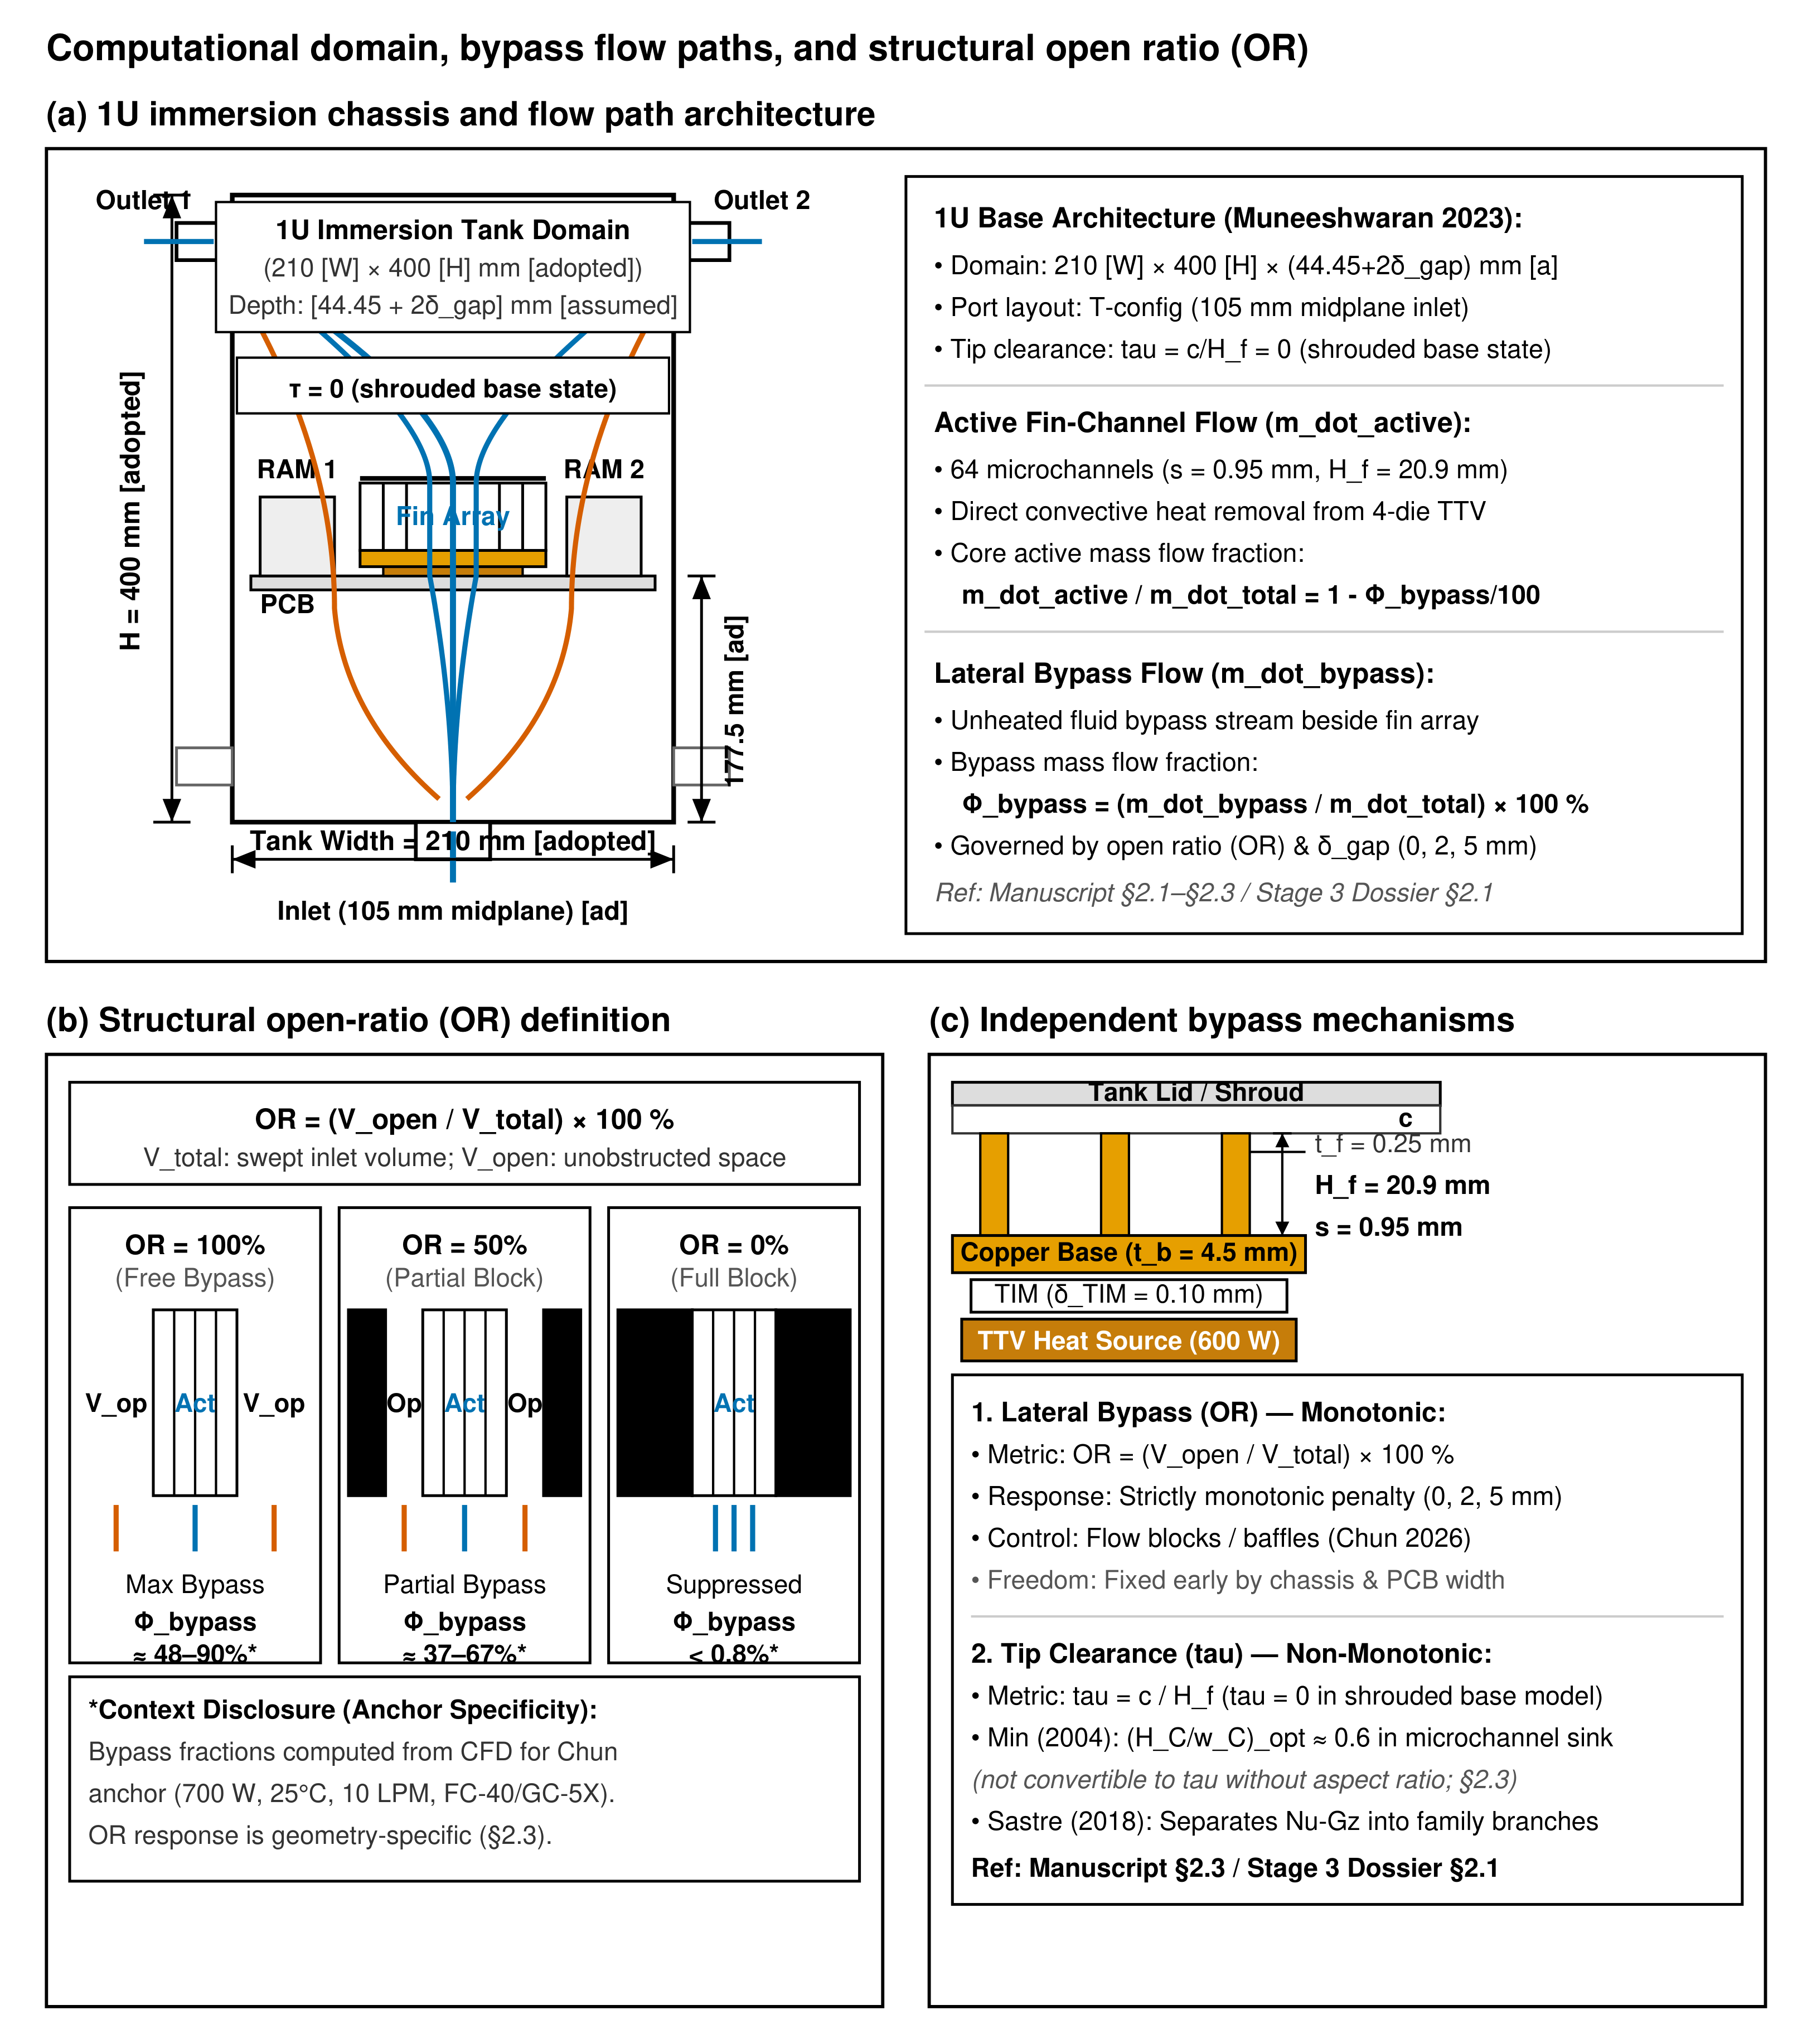
\includegraphics[width=\textwidth]{../figures/fig1_domain.png}
\caption{Computational domain, bypass flow paths and the open-ratio definition. (a) the 1U
immersion chassis with the active fin-channel flow and lateral bypass stream (with the shrouded
$\tau=0$ base state and independent tip clearance treated in panel (c)). (b) the open-ratio
definition at the heat-sink inlet plane across three blockage states. (c) lateral bypass and tip
clearance shown as the two independent mechanisms carried separately in this model, per
Section~\ref{sec:openratio}.}
\label{fig:domain}
\end{figure}

Table~\ref{tab:ledger-base} is the complete dimension ledger for the base model. Every row carries
one of three tags. A row tagged \texttt{[adopted]} is printed in the cited source at the cited
page, in body text, in a table, or as a dimension callout drawn on a figure. A row tagged
\texttt{[derived]} is computed from \texttt{[adopted]} rows, with the arithmetic shown. A row
tagged \texttt{[assumed]} is not available in any source consulted, and its value, its bounds and
the results it can move are stated in Section~\ref{sec:assumptions}. No row in the ledger is
digitised from a plot. Several of the \texttt{[adopted]} rows are recoverable only by rendering
the source page to an image and reading the drawing, because plain text extraction drops
dimension callouts that exist as vector labels inside a figure; those rows name the figure.

\begingroup
\footnotesize
\setlength{\tabcolsep}{4pt}
\begin{longtable}{@{}r>{\raggedright\arraybackslash}p{0.200\textwidth}c>{\raggedright\arraybackslash}p{0.135\textwidth}l>{\raggedright\arraybackslash}p{0.275\textwidth}@{}}
\caption{Dimension ledger for the base model, the 1U immersion server of Muneeshwaran et
al.~\cite{muneeshwaran2023}. Page numbers are the printed journal page of
\textit{Int.\ Commun.\ Heat Mass Transf.} \textbf{145} (2023) 106843, which coincides with the
PDF page index for this article.}
\label{tab:ledger-base}\\
\toprule
\# & Quantity & Symbol & Value & Tag & Source or arithmetic \\
\midrule
\endfirsthead
\multicolumn{6}{@{}l}{\normalfont\itshape Table~\ref{tab:ledger-base} continued}\\
\toprule
\# & Quantity & Symbol & Value & Tag & Source or arithmetic \\
\midrule
\endhead
\midrule
\multicolumn{6}{@{}r}{\normalfont\itshape continued on next page}\\
\endfoot
\bottomrule
\endlastfoot
1  & Rack unit height, server slot        &            & 44.45~mm & \texttt{[adopted]} & p.~1, abstract \\
2  & Heat-sink base thickness             & $t_b$      & 4.5~mm   & \texttt{[adopted]} & p.~3, \S2.1 \\
3  & Fin thickness                        & $t_f$      & 0.25~mm  & \texttt{[adopted]} & p.~3, \S2.1 \\
4  & Fin height                           & $H_f$      & 20.9~mm  & \texttt{[adopted]} & p.~3, \S2.1 \\
5  & Fin pitch, two builds                & $p_f$      & 1.2 and 2.2~mm & \texttt{[adopted]} & p.~3; Table~3, p.~7 \\
6  & Fin channel width                    & $s$        & 0.95~mm; 1.95~mm & \texttt{[derived]} & $s=p_f-t_f$ \\
7  & Channel hydraulic diameter           & $D_h$      & 1.817~mm; 3.567~mm & \texttt{[derived]} & $D_h=2sH_f/(s+H_f)$ \\
8  & Heat-sink stack height               & $t_b+H_f$  & 25.4~mm  & \texttt{[derived]} & $4.5+20.9$ \\
9  & Heat-sink base footprint             & $L\times W$& 118~mm $\times$ 78~mm & \texttt{[adopted]} & Fig.~2(b), p.~5, rendered callouts \\
10 & Raised finned-section callouts       &            & 81~mm and 31.2~mm & \texttt{[adopted]} & Fig.~2(b), p.~5. The drawing does not label which feature each callout terminates on \\
11 & Fin-bank plan area                   & $A_{bank}$ & 78~mm $\times$ 118~mm & \texttt{[assumed]} & Bounds 31.2 $\times$ 81~mm to 78 $\times$ 118~mm; see Section~\ref{sec:assumptions} \\
12 & Fin count, $p_f=1.2$~mm              & $N_f$      & 65 fins, 64 channels & \texttt{[derived]} & $Nt_f+(N-1)s=W$ on row 11 \\
13 & Fin count, $p_f=2.2$~mm              & $N_f$      & 36 fins, 35 channels & \texttt{[derived]} & same relation on row 11 \\
14 & Channel free-flow area, base build   & $A_c$      & $1.271\times10^{-3}$~m$^2$ & \texttt{[derived]} & $64\times0.95\times20.9$~mm$^2$ \\
15 & Heat-sink material                   &            & copper   & \texttt{[adopted]} & p.~3, \S2.1 \\
16 & Mock CPU package footprint           &            & 48~mm $\times$ 68~mm & \texttt{[adopted]} & Fig.~2(e), p.~7, rendered callouts \\
17 & Die count                            &            & 4, independently modulated & \texttt{[adopted]} & p.~3, \S2.1; Fig.~2(e), p.~7 \\
18 & Individual die footprint             &            & 2 $\times$ 2 tiling of a centred block & \texttt{[assumed]} & Bounds 50\% to 90\% of the package footprint; see Section~\ref{sec:assumptions} \\
19 & Thermal interface material           &            & grease TC-5888, $k=5.2$ &  \texttt{[adopted]} & p.~3, \S2.1; $k$ in W~m$^{-1}$~K$^{-1}$ \\
20 & TIM bond-line thickness              & $\delta_{TIM}$ & 0.10~mm & \texttt{[assumed]} & Bounds 0.05 to 0.20~mm; see Section~\ref{sec:assumptions} \\
21 & Bypass gap, heat sink to tank wall   & $\delta_{gap}$ & 0, 2, 5~mm & \texttt{[adopted]} & p.~5, \S3.2; Fig.~6, p.~9; Fig.~7, p.~10 \\
22 & Tank, long horizontal dimension      &            & 210~mm   & \texttt{[adopted]} & Fig.~2(c), p.~6, rendered callouts \\
23 & Tank, vertical dimension             &            & 400~mm   & \texttt{[adopted]} & Fig.~2(c), p.~6 \\
24 & Bottom inlet axis from tank end wall &            & 105~mm   & \texttt{[adopted]} & Fig.~2(c), p.~6; $105=210/2$, so the inlet is on the tank mid-plane \\
25 & Side port axes from floor and ceiling&            & 27.5~mm  & \texttt{[adopted]} & Fig.~2(c), p.~6 \\
26 & Heat-sink underside above tank floor &            & 177.5~mm & \texttt{[adopted]} & Fig.~2(c), p.~6 \\
27 & Tank depth, out-of-plane             &            & 44.45~mm internal $+\,2\delta_{gap}$ & \texttt{[assumed]} & Bounds 44.45 to 55~mm internal; see Section~\ref{sec:assumptions} \\
28 & Tank wall material                   &            & acrylic, adiabatic outer face & \texttt{[assumed]} & $k=0.19$; bounds 0.19 to 16.4~W~m$^{-1}$~K$^{-1}$; see Section~\ref{sec:assumptions} \\
29 & Server tray outline                  &            & 275 and 245~mm; 201 and 141.7~mm & \texttt{[adopted]} & Fig.~2(a), p.~5, rendered callouts \\
30 & Memory bank envelope                 &            & 149 $\times$ 59.3 $\times$ 34.1~mm; pitch 7.5~mm; gap 3.3~mm & \texttt{[adopted]} & Fig.~2(d), p.~6, rendered callouts \\
31 & Memory thermal load                  &            & zero, flow obstruction only & \texttt{[adopted]} & p.~3, \S2.1 \\
32 & PCB thickness                        &            & 2.4~mm   & \texttt{[assumed]} & From Khoshvaght-Aliabadi et al.~\cite{khoshvaghtaliabadi2026oblique}, Table~1, p.~5; bounds 1.6 to 3.0~mm \\
\end{longtable}
\endgroup

\begin{figure}[htbp]
\centering
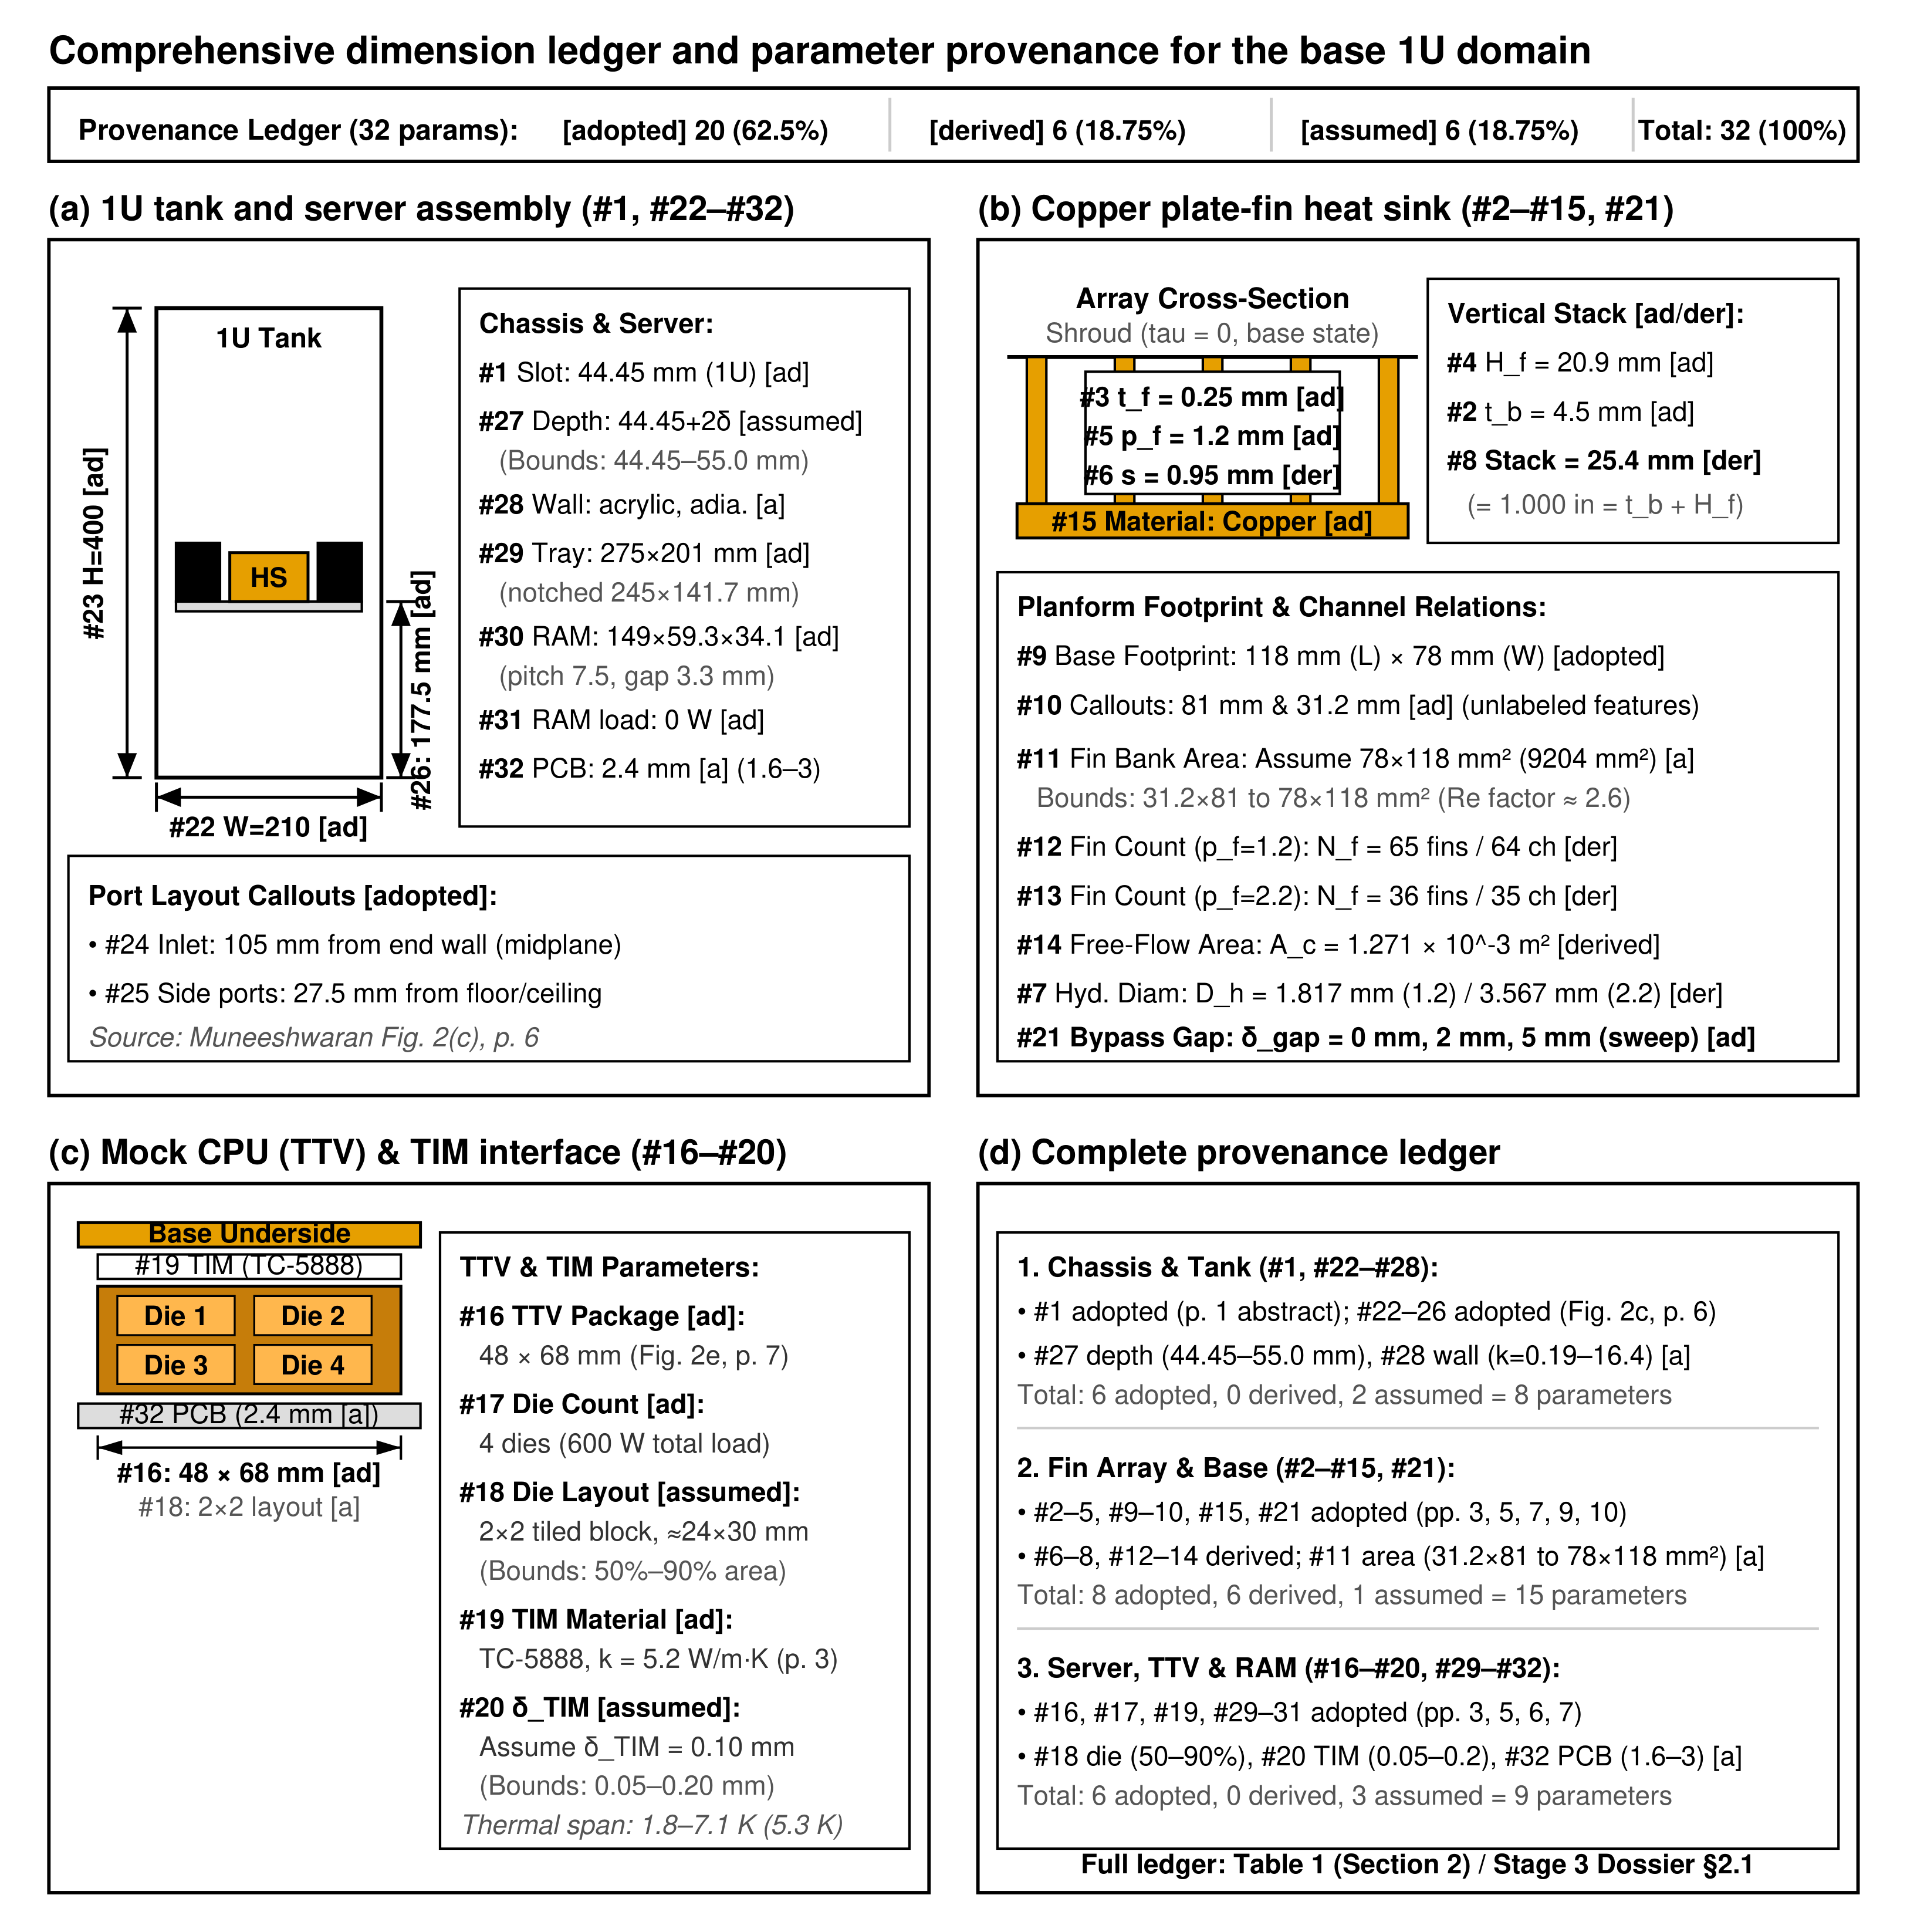
\includegraphics[width=\textwidth]{../figures/fig2_dimension_ledger.png}
\caption{Dimension ledger and parameter provenance for the base model geometry, matching
Table~\ref{tab:ledger-base}. Adopted, derived and assumed dimensions are visually distinguished
so that the source of every number in the model is visible at a glance.}
\label{fig:ledger}
\end{figure}

Two conventions follow from the ledger and are stated here so that no downstream quantity is
ambiguous. First, the fin bank is taken to span the 78~mm base width, so the span sets the channel
count and the 118~mm base length is the channel flow length. Second, the channel hydraulic
diameter of row 7 is the length scale for every Reynolds and Nusselt number reported in this
paper. That second point needs saying because the bypass and tip-clearance literature this work
builds on does not share a convention: Sastre et al.~\cite{sastre2018} use the hydraulic diameter
of the finned cross-section including the clearance slab, Mei et al.~\cite{mei2014} use the pin
diameter with the maximum velocity, Jeng~\cite{jeng2008} uses the bare rectangular duct with the
inlet velocity, Shahsavar et al.~\cite{shahsavar2021} use four times the array volume over its
wetted area, Shrigondekar et al.~\cite{shrigondekar2023} use the bare fin spacing, and Min et
al.~\cite{min2004} report no Reynolds number at all and sweep pumping power instead. Five
incompatible length scales across six papers is a large part of why no dimensionless framework for
this problem exists yet, and every literature value quoted in this paper is recomputed on the
convention above before it is compared with anything.

Applying that convention to the base geometry gives a channel Reynolds number
$\mathrm{Re}_{ch}=\dot{m}D_h/(A_c\mu)$ of roughly 5 to 122 over the 1 to 3~LPM flow range and the
15 to 35~$^{\circ}$C inlet range, if all flow is forced through the fins. The band is wide, and it
is wide for an honest reason: it carries the factor of about 2.6 between the two bounds of the
fin-bank span in row 11. No single-valued channel Reynolds number is quoted for the base geometry
anywhere in this paper. The one directly printed check available is Shrigondekar et
al.~\cite{shrigondekar2023}, who report a fin-spacing Reynolds number of about 10 to 70 for FC-40
on the same rig at the same flow rates and the same two fin pitches. Converted onto the fin-spacing
length scale, the wide-span bound of row 11 gives 2.5 to 46 and the narrow-span bound gives 6.4 to
114. The printed value therefore sits inside the narrow band and partly above the wide one, which
means this check leans against the value adopted rather than confirming it. That is recorded here
rather than smoothed over.

\subsection{Reference configuration for the anchor comparison}
\label{sec:v3}

A second, fully dimensioned geometry is carried alongside the base model so that the open-ratio
results of Chun et al.~\cite{chun2026} can be reproduced without rescaling anything.
Table~\ref{tab:ledger-v3} is its ledger. It is not a substitute for the base model and no result
from the two configurations is pooled.

\begingroup
\footnotesize
\setlength{\tabcolsep}{4pt}
\begin{longtable}{@{}l>{\raggedright\arraybackslash}p{0.225\textwidth}>{\raggedright\arraybackslash}p{0.185\textwidth}l>{\raggedright\arraybackslash}p{0.245\textwidth}@{}}
\caption{Dimension ledger for the reference configuration used in the anchor comparison, the 1U
plate-fin build of Chun et al.~\cite{chun2026}. Page numbers are the printed journal page of
\textit{Energy} \textbf{361} (2026) 141967.}
\label{tab:ledger-v3}\\
\toprule
\# & Quantity & Value & Tag & Source or arithmetic \\
\midrule
\endfirsthead
\multicolumn{5}{@{}l}{\normalfont\itshape Table~\ref{tab:ledger-v3} continued}\\
\toprule
\# & Quantity & Value & Tag & Source or arithmetic \\
\midrule
\endhead
\midrule
\multicolumn{5}{@{}r}{\normalfont\itshape continued on next page}\\
\endfoot
\bottomrule
\endlastfoot
A1  & 1U internal slot spacing        & 44.45~mm & \texttt{[adopted]} & p.~5, \S2.1 \\
A2  & Fin thickness                   & 2~mm     & \texttt{[adopted]} & Fig.~2(a), p.~5, callout under a ``Unit : mm'' header \\
A3  & Fin spacing                     & 3~mm     & \texttt{[adopted]} & Fig.~2(a), p.~5 \\
A4  & Fin height                      & 20~mm    & \texttt{[adopted]} & Fig.~2(a), p.~5 \\
A5  & Fin pitch                       & 5~mm     & \texttt{[derived]} & $2+3$ \\
A6  & Heat-sink base plate            & 72~mm width $\times$ 106~mm flow length & \texttt{[adopted]} & Fig.~2(a), p.~5 \\
A7  & Fin count                       & 15 fins, 14 channels & \texttt{[derived]} & $2N+3(N-1)=72$ gives $N=15$ exactly \\
A8  & Channel free-flow area          & $8.40\times10^{-4}$~m$^2$ & \texttt{[derived]} & $14\times3\times20$~mm$^2$ \\
A9  & Channel hydraulic diameter      & 5.217~mm & \texttt{[derived]} & $2(3)(20)/23$ \\
A10 & Copper block, mock CPU          & 50 $\times$ 65 $\times$ 8~mm & \texttt{[adopted]} & Fig.~2(a), p.~5 \\
A11 & TIM, indium foil thickness      & $\approx$0.1~mm & \texttt{[adopted]} & p.~6, \S2.1 \\
A12 & Heat-sink centre spacing on PCB & 60~mm    & \texttt{[adopted]} & p.~6, \S2.1, and Fig.~2(a), p.~5 \\
A13 & Tank internal width             & 423~mm   & \texttt{[adopted]} & Fig.~2(a), p.~5, right-hand panel headed ``Immersion tank'' \\
A14 & Tank internal height, outlet plane to distribution-plate plane & 430~mm & \texttt{[adopted]} & Fig.~2(a), p.~5, right-hand panel \\
A15 & Distribution plate, 1U build    & 10 holes, 10~mm diameter & \texttt{[adopted]} & p.~5, \S2.1 \\
A16 & Distribution plate, 3U build    & 30 holes, 5~mm diameter & \texttt{[adopted]} & p.~5, \S2.1 \\
A17 & Tank material                   & SUS304, double-layer insulation, tempered-glass window & \texttt{[adopted]} & p.~4, \S2.1; properties Table~2, p.~6 \\
A18 & Flow-control block material     & acrylic  & \texttt{[adopted]} & p.~6, \S2.1 \\
A19 & Flow-control block dimensions   & not dimensioned in the source & \texttt{[assumed]} & The open ratio is therefore defined here by the volume a block occludes, never by a block dimension \\
A20 & Tank external envelope          & not printed in the source & \texttt{[assumed]} & Not required: the computational domain is the wetted interior bounded by A13, A14 and A1 \\
A21 & Metal-foam alternative core     & 10~PPI, porosity 0.9; sweep 5 to 15~PPI, porosity 0.5 to 0.9 & \texttt{[adopted]} & p.~15 and p.~18, \S3.3 \\
\end{longtable}
\endgroup

Three specific gaps in this reference configuration are carried openly rather than closed
silently, because an independent reproducibility check found them and they are real. The source
does not print the tank's third, out-of-plane dimension, does not print the heat-sink base
thickness, and does not give the numerical inlet profile, outlet type or tank-wall thermal
condition, so the anchor comparison in Section~\ref{sec:verification} is a best-effort check
against a paper that does not fully close its own specification, not a fully reproducible
benchmark. The same three gaps are the reason A19, A20 and the base thickness never enter a
reported quantity.

\subsection{Open ratio}
\label{sec:openratio}

The bypass metric is adopted verbatim from Chun et al.~\cite{chun2026}, who introduce it as an
unnumbered display equation on their p.~11 and illustrate it in their Fig.~8. Their words for it,
quoted so that nothing is quietly reinterpreted here, are that the open ratio is
\textit{the volumetric fraction of the unobstructed fluid inlet space relative to the total heat
sink inlet volume}:

\begin{equation}
\mathrm{OR} = \frac{V_{\mathrm{open}}}{V_{\mathrm{total}}}\times 100 \quad (\%)
\label{eq:or}
\end{equation}

\noindent
Named for the geometry of Table~\ref{tab:ledger-base}, the two volumes in Eq.~(\ref{eq:or}) are
the following. $V_{\mathrm{total}}$ is the total heat-sink inlet volume, the fluid volume swept
out by the heat-sink inlet plane over the inlet-plane thickness, that is the plan area of the 1U
slot facing the heat sink multiplied by the inlet-plane thickness, spanning the full tank width
available to the flow at that height. $V_{\mathrm{open}}$ is the unobstructed fluid inlet space,
the part of $V_{\mathrm{total}}$ occupied by neither the heat sink nor a flow-control block, that
is the volume through which fluid can reach the outlets without passing between the fins. At
$\mathrm{OR}=100\%$ the tank is unobstructed and bypass is free. At $\mathrm{OR}=0\%$ every
entering parcel is directed through the heat-source region.

Three properties of the definition travel with it, because dropping any of them changes what the
number means. It is a volume ratio at the inlet plane, not an area ratio and not a clearance in
millimetres; the source never converts it to a gap width. It is geometry-specific, and the source
says so, so any open ratio quoted here travels with the geometry it was measured on. And the
blocking acts laterally, from both edges symmetrically, which in the 1U build means the top gap is
absent and the open ratio is a purely lateral quantity.

Open ratio is a geometric input. Its companion output, also taken from
Chun et al.~\cite{chun2026}, is the bypass mass fraction,

\begin{equation}
\dot{m}_{\mathrm{bypass}} = \dot{m}_{\mathrm{total}} - \dot{m}_{\mathrm{active}},
\qquad
\Phi_{\mathrm{bypass}} = \frac{\dot{m}_{\mathrm{bypass}}}{\dot{m}_{\mathrm{total}}}\times 100
\quad (\%),
\label{eq:phibypass}
\end{equation}

\noindent
where the bypass region is the flow region excluding the heat-sink passages and the region
directed toward the heat source. This paper reports $\mathrm{OR}$ as the design variable and
$\Phi_{\mathrm{bypass}}$ as the computed response, in the same pairing the source uses.

Lateral bypass and tip clearance are carried as two separate parameters and are never combined
into one scalar. The tip clearance ratio is defined as

\begin{equation}
\tau = \frac{c}{H_f},
\label{eq:tau}
\end{equation}

\noindent
the clearance height over the fin height, and is held at $\tau=0$ in the base configuration. Four
reasons keep the two apart. The 1U build that defines the open ratio has already eliminated the
top gap, so folding a tip term into it would redefine the source's own quantity while keeping its
name. No study surveyed here varies both mechanisms; every tip-clearance study varies only the tip
gap and both side-bypass studies vary only the side gap, so a combined ratio would be a quantity
with no supporting measurement anywhere. Jeng~\cite{jeng2008} argues the point directly, noting
that the tip gap dominates in magnitude and can be changed late in a design while the channel
width is fixed early by the board width, which in a 1U immersion chassis holds with extra force.
And the two responses have different shapes. Tip clearance is non-monotonic and has an interior
optimum: Min et al.~\cite{min2004} report a minimum thermal resistance of 0.058~$^{\circ}$C~W$^{-1}$
at a clearance-to-channel-width ratio of 0.6 under 2.27~W of pumping power, and Mei et
al.~\cite{mei2014} report the same competing-effects reversal. Lateral bypass is monotonic and
always detrimental, in Muneeshwaran et al.~\cite{muneeshwaran2023} across the 0 to 5~mm gap sweep
and in Chun et al.~\cite{chun2026} across the open-ratio sweep. Collapsing a bounded parameter
with an optimum and a monotone detrimental one into a single scalar would make any interior
optimum in the combined ratio unattributable to either mechanism. Sastre et al.~\cite{sastre2018}
supply the warning empirically: even one clearance parameter was strong enough to split their
Nusselt-Graetz curves into separate families rather than one fit.

One out-of-sample check on the open ratio exists and is used. Jeng~\cite{jeng2008} parameterises
lateral bypass around a square pin-fin sink as the ratio $W/L$ of channel width to sink length. For
a constant-height inlet plane the two parameterisations map exactly, $\mathrm{OR} = (1-L/W)\times
100$, so $W/L$ of 1, 2, 3 and 5 correspond to open ratios of 0, 50, 66.7 and 80\%. Jeng's
recommendation of $W/L$ between 2 and 3 therefore sits inside the range swept here, in a different
fluid and a different fin type. The mapping is derived here, not printed in either source, and it
holds only when the open volume is the lateral space at the same inlet-plane height.

\subsection{Working fluids and thermophysical properties}
\label{sec:properties}

Two dielectric coolants are used. FC-40, a perfluorinated fluorocarbon, is the primary fluid: it is
the one coolant for which more than one independent group in this literature has published usable
property data, so a property error can be caught by cross-checking rather than trusted. GC-5X, an
oil-based dielectric, is the high-viscosity contrast case. Carrying two fluids is not decoration.
Chun et al.~\cite{chun2026} show that open-ratio sensitivity is a strong function of viscosity,
with thermal resistance falling 6.1\% for FC-40 but 45.6\% for GC-5X as the bypass is closed, so a
framework claimed to be dimensionless must be exercised across more than one Prandtl decade or the
claim is untested.

Table~\ref{tab:fluidprops} gives the property treatment and the source of every value.

\begin{table}[htbp]
\centering
\caption{Coolant thermophysical properties and their sources. The correlations of Chun et
al.~\cite{chun2026} take $T$ in kelvin; see the discussion below.}
\label{tab:fluidprops}
\footnotesize
\setlength{\tabcolsep}{4pt}
\begin{tabular}{@{}l>{\raggedright\arraybackslash}p{0.105\textwidth}>{\raggedright\arraybackslash}p{0.405\textwidth}>{\raggedright\arraybackslash}p{0.215\textwidth}@{}}
\toprule
Fluid & Property & Value or correlation ($T$ in K) & Source \\
\midrule
FC-40 & $\rho$    & $2499 - 2.16\,T$~kg~m$^{-3}$ & \cite{chun2026}, Table~3, p.~7 \\
FC-40 & $k$       & $0.086 - 6.90\times10^{-5}\,T$~W~m$^{-1}$~K$^{-1}$ & \cite{chun2026}, Table~3, p.~7 \\
FC-40 & $c_p$     & $590 + 1.55\,T$~J~kg$^{-1}$~K$^{-1}$ & \cite{chun2026}, Table~3, p.~7 \\
FC-40 & $\mu$     & $0.0429 - 0.162\times10^{-3}\,T$ $+\;1.08\times10^{-7}\,T^2$~Pa~s & \cite{chun2026}, Table~3, p.~7 \\
FC-40 & $\rho$ & 1874.44~kg~m$^{-3}$ at 16~$^{\circ}$C & \cite{muneeshwaran2023}, Table~4, p.~7 \\
FC-40 & $\nu$ & $5\times10^{-6}$, $1.5\times10^{-6}$, $5.4\times10^{-7}$~m$^2$~s$^{-1}$ at 0, 40, 100~$^{\circ}$C & \cite{muneeshwaran2023}, Table~4, p.~7 \\
FC-40 & $c_p$ & 1014, 1076, 1169.4~J~kg$^{-1}$~K$^{-1}$ at 0, 40, 100~$^{\circ}$C & \cite{muneeshwaran2023}, Table~4, p.~7 \\
FC-40 & $k$ & 0.067, 0.0642, 0.0601~W~m$^{-1}$~K$^{-1}$ at 0, 40, 100~$^{\circ}$C & \cite{muneeshwaran2023}, Table~4, p.~7 \\
FC-40 & $\beta$   & $1.2\times10^{-3}$~K$^{-1}$ & \cite{muneeshwaran2023}, Table~4, p.~7 \\
FC-40 & Boiling pt. & 165~$^{\circ}$C at 1~bar & \cite{muneeshwaran2023}, Table~4, p.~7 \\
FC-40 & $\mathrm{Pr}$ & 67.5 at 25~$^{\circ}$C & \texttt{[derived]} from the correlations above \\
\midrule
GC-5X & $\rho$    & $1049.862 - 0.75\,T$~kg~m$^{-3}$ & \cite{chun2026}, Table~3, p.~7 \\
GC-5X & $k$       & $0.199367 - 1.8\times10^{-4}\,T$~W~m$^{-1}$~K$^{-1}$ & \cite{chun2026}, Table~3, p.~7 \\
GC-5X & $c_p$     & $2076.055 + 0.3\,T$~J~kg$^{-1}$~K$^{-1}$ & \cite{chun2026}, Table~3, p.~7 \\
GC-5X & $\mu$     & $0.6449 - 4.1234\times10^{-3}\,T$ $+\;8.9697\times10^{-6}\,T^2$ $-\;6.5833\times10^{-9}\,T^3$~Pa~s & \cite{chun2026}, Table~3, p.~7 \\
GC-5X & $\beta$   & $9.08\times10^{-4}$~K$^{-1}$ at 25~$^{\circ}$C & \texttt{[derived]}, $\beta=-\rho^{-1}\partial\rho/\partial T$ on the density fit of this table. No measured value is printed in any source consulted \\
GC-5X & $\mathrm{Pr}$ & 570 at 25~$^{\circ}$C & \texttt{[derived]} from the correlations above \\
\bottomrule
\end{tabular}
\end{table}

Two findings about these properties came out of checking them rather than copying them, and both
change how the correlations may be used.

The first is that the correlations of Chun et al.~\cite{chun2026} take $T$ in kelvin, which their
paper does not state and their own nomenclature contradicts by defining $T$ in degrees Celsius.
The evidence is arithmetic and it is decisive. With $T$ in kelvin the FC-40 density fit returns
1874.4~kg~m$^{-3}$ at 289.15~K, against the 1874.44~kg~m$^{-3}$ at 16~$^{\circ}$C measured
independently by Muneeshwaran et al.~\cite{muneeshwaran2023}. The conductivity fit returns 0.0672,
0.0644 and 0.0603~W~m$^{-1}$~K$^{-1}$ at 0, 40 and 100~$^{\circ}$C against their printed 0.067,
0.0642 and 0.0601, and the specific-heat fit returns 1013.4, 1075.4 and 1168.4~J~kg$^{-1}$~K$^{-1}$
against their printed 1014, 1076 and 1169.4. Three properties agree to better than 0.1\% at three
temperatures each on one unit convention and are irreconcilable on the other. The same conclusion
follows independently from the source's own mass-flow table, which converts to exactly 5.00~LPM per
heat sink at the stated 10~LPM for two heat sinks only when the density is evaluated in kelvin.
This is an inference from the paper's numbers, not a printed statement, and it should be confirmed
with the corresponding author before any anchor result is reproduced.

The second finding is a limit on the FC-40 viscosity fit, and it constrains the model. That
quadratic reaches zero at about 343~K, or 70~$^{\circ}$C, and is negative above it, so it cannot be
used at wall temperatures approaching the 80~$^{\circ}$C case-temperature limit of the base
paper~\cite{muneeshwaran2023}. Within its useful band it is good: against the kinematic-viscosity
points of Muneeshwaran et al.\ interpolated logarithmically it agrees to 1.2\% at 35~$^{\circ}$C
and 3.9\% at 25~$^{\circ}$C, degrading to 13\% at 15~$^{\circ}$C and 30\% at 0~$^{\circ}$C. FC-40
viscosity is therefore evaluated from the fit between 20 and 60~$^{\circ}$C and from the measured
points of Muneeshwaran et al.\ outside that band. The GC-5X cubic stays positive and monotone
across the whole range of interest and needs no such restriction.

Solid properties are listed in Table~\ref{tab:solidprops}. Where two sources print a value, both
are named, and where they agree exactly that is said, because agreement between independently
published tables is the only property check available in the absence of a measurement of our own.

\begin{table}[htbp]
\centering
\caption{Solid domain properties and their sources. Density in kg~m$^{-3}$, specific heat in J~kg$^{-1}$~K$^{-1}$, thermal conductivity in W~m$^{-1}$~K$^{-1}$.}
\label{tab:solidprops}
\footnotesize
\setlength{\tabcolsep}{4pt}
\begin{tabular}{@{}>{\raggedright\arraybackslash}p{0.155\textwidth}cc>{\raggedright\arraybackslash}p{0.105\textwidth}>{\raggedright\arraybackslash}p{0.30\textwidth}@{}}
\toprule
Domain & $\rho$ & $c_p$ & $k$ & Source \\
\midrule
Copper, fins and base & 8978 & 381 & 387.6 & \cite{chun2026}, Table~2, p.~6; the identical triplet is printed independently in \cite{khoshvaghtaliabadi2026oblique}, Table~1, p.~5 \\
TIM, base model, thermal grease & \multicolumn{2}{c}{not printed} & 5.2 & \cite{muneeshwaran2023}, p.~3, \S2.1 \\
TIM, reference configuration, indium & 7310 & 234 & 81.8 & \cite{chun2026}, Table~2, p.~6 \\
PCB substrate & 1850 & 1000 & 0.3 & \cite{khoshvaghtaliabadi2026oblique}, Table~1, p.~5 \\
PCB substrate, alternative & 3600 & 720 & 42.0 in-plane, 0.5 cross-plane & \cite{chun2026}, Table~2, p.~6 \\
SUS304, reference configuration tank & 8000 & 500 & 16.4 & \cite{chun2026}, Table~2, p.~6 \\
Acrylic, flow-control block and tank wall & 1180 & 1460 & 0.21 & \cite{chun2026}, Table~2, p.~6 \\
\bottomrule
\end{tabular}
\end{table}

The two PCB entries disagree by two orders of magnitude in conductivity because they describe
different things: one is an isotropic bulk laminate value, the other resolves the copper-plane
anisotropy. The isotropic entry is used for the base model, where the board is an unloaded
conduction path, and the anisotropic entry is used for the anchor comparison so that the
reference configuration keeps its own source's convention. Neither value moves a reported quantity
in this work, since the board carries no thermal load in the base model. All solid property values
in Table~\ref{tab:solidprops} are attributed within their source to further references rather than
measured there, and are carried on that basis.

\subsection{Assumptions}
\label{sec:assumptions}

Eight quantities in Tables~\ref{tab:ledger-base} and \ref{tab:ledger-v3} are not available in any
source consulted. Each is listed below with the value taken, the reason, the defensible bounds and
the results it can move. Nothing here is assumed because it was convenient, and nothing that a
result depends on is hidden inside a sentence.

\noindent\textbf{Fin-bank plan area, 78~mm $\times$ 118~mm (row 11).}\ The base outline of the heat sink is
dimensioned but the drawing does not label which feature its two interior callouts, 81~mm and
31.2~mm, terminate on. Bounds are therefore 31.2 $\times$ 81~mm at the low end and 78 $\times$
118~mm at the high end, a factor of 3.6 in plan area. The wide value is taken because it is the
only one under which the 48 $\times$ 68~mm mock-processor footprint of row 16 is fully covered by
the fin array. The counter-evidence is stated in Section~\ref{sec:geometry} and is not resolved:
converting the printed fin-spacing Reynolds range of Shrigondekar et al.~\cite{shrigondekar2023}
onto this geometry leans toward the narrow bound. Results moved: the span sets the channel count,
64 channels at 78~mm against 25 at 31.2~mm, hence a free-flow area of 1271~mm$^2$ against
496~mm$^2$, a factor of about 2.6 on channel velocity and on channel Reynolds number. Every
Reynolds number quoted for the base model carries that factor as a band. Thermal resistance is far
less sensitive, since the area enters through fin efficiency and total wetted area rather than
linearly. This is the largest single geometric uncertainty in the model, and the cheapest way to
settle it is a higher-resolution copy of the source drawing or a question to its corresponding
author.

\noindent\textbf{Die partition inside the mock-processor package (row 18).}\ The four dies are drawn as a
tiled block but the block is not dimensioned. Bounds are a die block between 50\% and 90\% of the
48 $\times$ 68~mm package footprint. The assumption is low-risk because the heat load is applied as
a boundary condition at the heat-sink base, following the base paper's own numerical
treatment~\cite{muneeshwaran2023}, so the die partition never enters the model. Results moved: only
a local peak junction temperature post-process, which this paper does not report.

\noindent\textbf{TIM bond-line thickness, 0.10~mm (row 20).}\ The base paper names the grease and gives its
conductivity but not the bond line. The value is set to match the indium-foil thickness printed for
the reference configuration~\cite{chun2026} so that both configurations share one interface
convention. Bounds 0.05 to 0.20~mm, the usual range for a screwed-down grease line. Results moved:
absolute case temperature shifts by about 5.3~K across those bounds ($-1.8$~K to $+3.5$~K relative to
the 0.10~mm nominal) at 600~W over the row 16 footprint. Thermal-resistance differences between open
ratios are insensitive to it, because it is a series resistance common to every case.

\noindent\textbf{Tank depth, 44.45~mm internal plus twice the bypass gap (row 27).}\ Genuinely absent. The tank
drawing carries no callout for the out-of-plane thickness and the body text gives none. The value
is chosen so that the tank interior is exactly the 1U slot the source's own abstract specifies.
Bounds 44.45 to 55~mm internal. Results moved: this dimension sets the bypass area and therefore
is the open ratio. It is the most consequential assumption in the ledger, and it is precisely why
this paper parameterises on the dimensionless open ratio rather than on an absolute tank depth.

\noindent\textbf{Tank wall material and outer boundary (row 28).}\ The base paper never names the tank material.
Acrylic with $k = 0.19$~W~m$^{-1}$~K$^{-1}$ is taken, consistent with the transparent wall in the
source's own photograph, with an adiabatic outer face. Bounds on $k$ run from 0.19 for acrylic to
16.4~W~m$^{-1}$~K$^{-1}$ for the stainless steel used in the reference
configuration~\cite{chun2026}. Results moved: none of those reported. The adiabatic outer face is
the source's own stated condition, since it reports that the entire experimental system was
insulated and that the heat loss was negligible~\cite{muneeshwaran2023}.

\noindent\textbf{PCB thickness, 2.4~mm (row 32).}\ Not given by the base paper. Taken from the only printed
PCB thickness available for a 1U immersion server~\cite{khoshvaghtaliabadi2026oblique}. Bounds 1.6
to 3.0~mm. Results moved: none reported here; the board is an unloaded conduction path of
$k \approx 0.3$~W~m$^{-1}$~K$^{-1}$.

\noindent\textbf{Flow-control block dimensions in the reference configuration (row A19).}\ The blocks are shown
schematically in the source but given no size. The open ratio is therefore defined by the volume a
block occludes, as in Eq.~(\ref{eq:or}), never by a block dimension. Results moved: the mapping
from open ratio to bypass fraction. Since this paper reports the open ratio as an input and the
bypass fraction as a computed output, no reported quantity requires the block geometry.

\noindent\textbf{External tank envelope in the reference configuration (row A20).}\ Not printed. Not required,
because the computational domain is the wetted interior bounded by rows A13, A14 and A1.

A separate set of quantities is held fixed rather than assumed, and each is fixed for a stated
reason. The rack unit height is held at 44.45~mm because it is an industry dimensional standard
printed identically by three independent groups~\cite{muneeshwaran2023,chun2026,kim2025}; it is not
a free design variable, and Kim et al.\ already swept it from 0.8U to 1.2U if a sensitivity
precedent is wanted. The mock-processor footprint is held at 48 $\times$ 68~mm because fixing the
heat-source footprint is what makes the open ratio the only varying geometric quantity; if the
footprint moved, a change in thermal resistance could not be attributed to bypass. The heat-sink
base thickness is held at 4.5~mm because it sets spreading resistance, which sits in series with
the convective resistance the open ratio acts on, so holding it keeps the two separable. The fin
material is held at copper: with a solid-to-fluid conductivity ratio near 6000 for FC-40, fin
efficiency is near unity and the result is insensitive to the copper grade, whereas switching to
aluminium would change fin efficiency and confound the bypass conclusion. The port arrangement is
held at the T-configuration because the base paper shows it is a first-order effect, 12.6\% in
thermal resistance against the Z-configuration, and because under the Z-configuration most of the
fluid bypasses the heat sink anyway; holding it removes a competing bypass mechanism so that the
open ratio is the only one varied~\cite{muneeshwaran2023}.

Fin pitch is deliberately not held constant. It is a second factor at the two printed levels of
1.2 and 2.2~mm, because the pitch and bypass interact: the penalty for opening the gap from 0 to
5~mm is 3\% at the coarse pitch but 7.4\% at the fine one~\cite{muneeshwaran2023}. The coolant is
deliberately not held constant either, for the Prandtl-range reason given in
Section~\ref{sec:properties}.
.
%
% PACKAGES REQUIRED IN main.tex PREAMBLE (not currently present):
%   \usepackage{booktabs}
%   \usepackage{array}      (for the >{\raggedright\arraybackslash}p{} column type)
% =============================================================================

\section{Problem formulation}
\label{sec:formulation}

\subsection{Base geometry}
\label{sec:geometry}

The model geometry is the 1U immersion server of Muneeshwaran et al.~\cite{muneeshwaran2023}:
a copper plate-fin heat sink clamped to a four-die thermal test vehicle on a printed circuit
board, with a bank of non-dissipating memory modules alongside it, the whole tray submerged in a
sealed 1U tank. Coolant enters through a port on the tank floor directly beneath the heat sink
and leaves through two ports at the top of the opposite faces, the arrangement those authors call
the T-configuration. That choice of base is not a matter of taste. It is the only 1U immersion
architecture in the surveyed literature whose server tray, heat sink, tank, memory bank and mock
processor all carry printed dimension callouts, so the domain can be rebuilt without scaling
anything off a figure. It is also the architecture that Chun et al.~\cite{chun2026} identify as
prior bypass-control work, that B. Zhang et al.~\cite{zhang2026} state they reconstructed as their
own computational domain, that Khoshvaght-Aliabadi and co-workers rebuilt twice as a validation
replica~\cite{khoshvaghtaliabadi2026oblique,khoshvaghtaliabadi2026component}, and from which Kim
et al.~\cite{kim2025} took their inlet and outlet arrangement. Only the first of those four is a
reuse of the architecture as a study domain; the others are weaker forms of reliance and are
described here as such.

The bypass mechanism this paper is about is present in the base paper and was measured there.
Muneeshwaran et al.~\cite{muneeshwaran2023} swept the clearance between the heat sink and the 1U
tank inner wall at 5, 2 and 0~mm, reported a 3\% to 7.4\% rise in thermal resistance and a
0.7~$^{\circ}$C to 1.5~$^{\circ}$C rise in case temperature as the gap opened, and adopted the
no-gap build for everything that followed. Their flow visualisation shows the reason: fluid takes
the clearance because its hydraulic resistance is lower, and that stream does no useful heat
transfer. The open ratio of Section~\ref{sec:openratio} is the dimensionless generalisation of
exactly this clearance.

\begin{figure}[htbp]
\centering
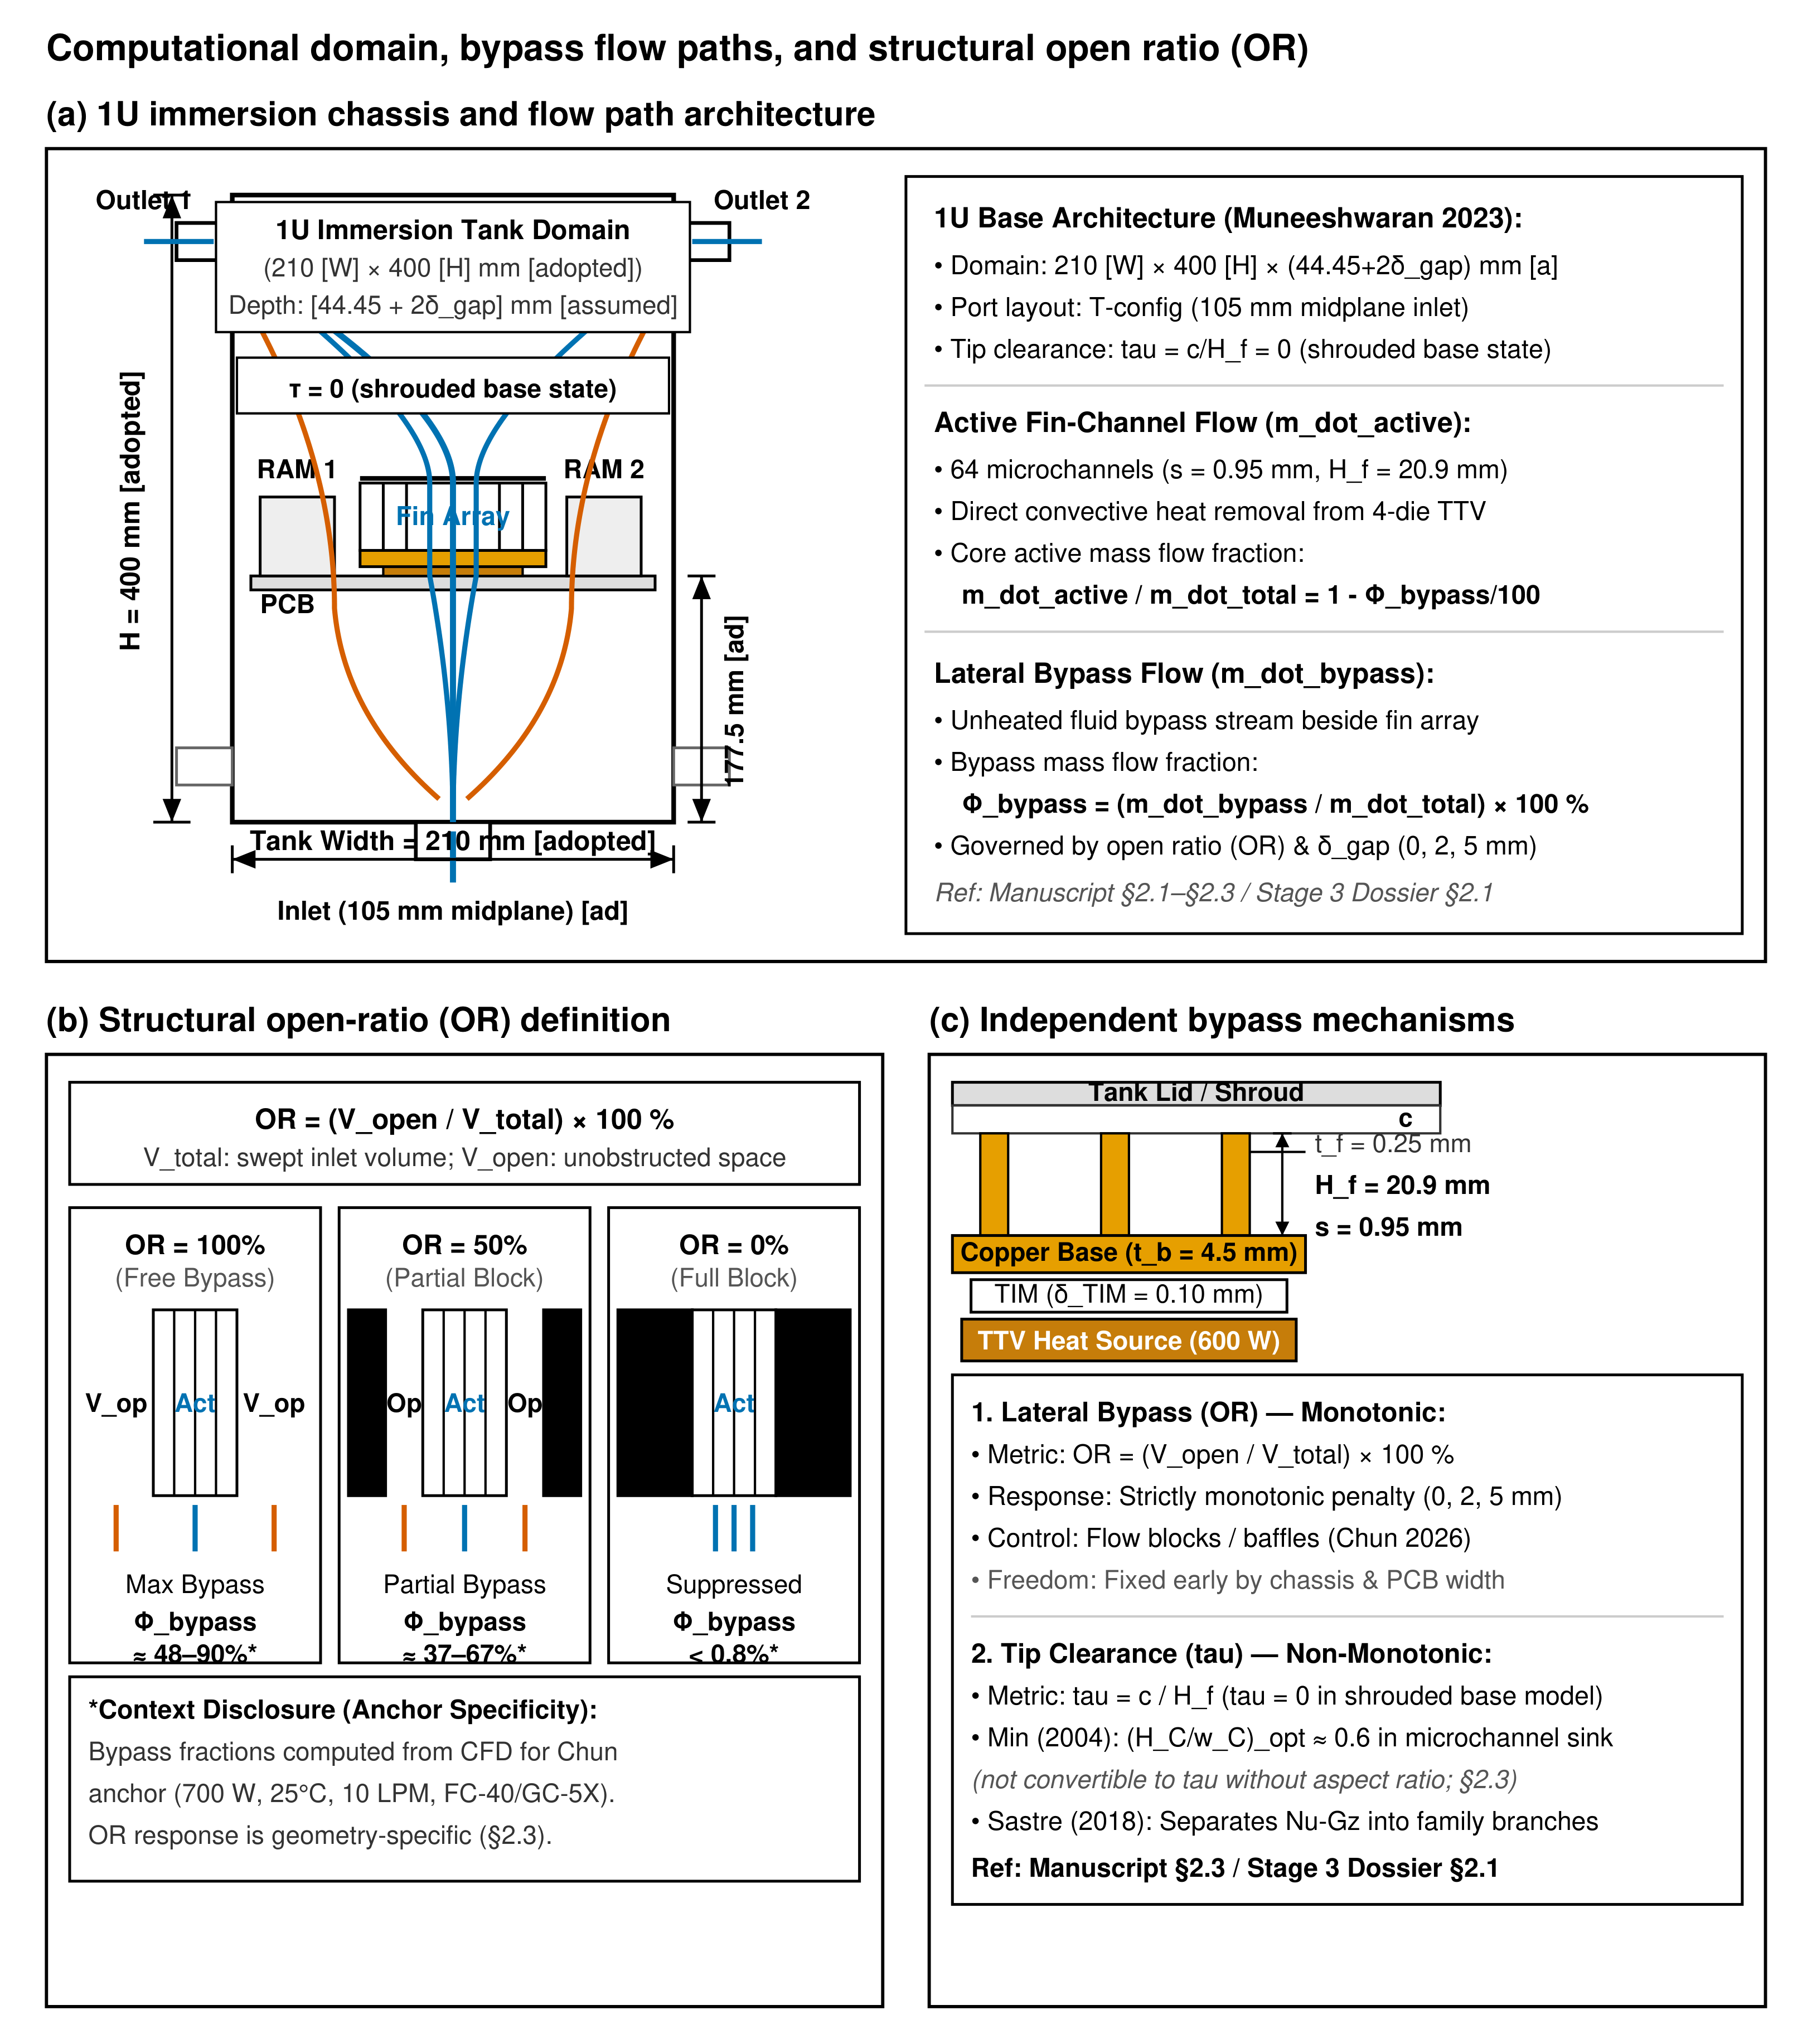
\includegraphics[width=\textwidth]{../figures/fig1_domain.png}
\caption{Computational domain, bypass flow paths and the open-ratio definition. (a) the 1U
immersion chassis with the active fin-channel flow and lateral bypass stream (with the shrouded
$\tau=0$ base state and independent tip clearance treated in panel (c)). (b) the open-ratio
definition at the heat-sink inlet plane across three blockage states. (c) lateral bypass and tip
clearance shown as the two independent mechanisms carried separately in this model, per
Section~\ref{sec:openratio}.}
\label{fig:domain}
\end{figure}

Table~\ref{tab:ledger-base} is the complete dimension ledger for the base model. Every row carries
one of three tags. A row tagged \texttt{[adopted]} is printed in the cited source at the cited
page, in body text, in a table, or as a dimension callout drawn on a figure. A row tagged
\texttt{[derived]} is computed from \texttt{[adopted]} rows, with the arithmetic shown. A row
tagged \texttt{[assumed]} is not available in any source consulted, and its value, its bounds and
the results it can move are stated in Section~\ref{sec:assumptions}. No row in the ledger is
digitised from a plot. Several of the \texttt{[adopted]} rows are recoverable only by rendering
the source page to an image and reading the drawing, because plain text extraction drops
dimension callouts that exist as vector labels inside a figure; those rows name the figure.

\begingroup
\footnotesize
\setlength{\tabcolsep}{4pt}
\begin{longtable}{@{}r>{\raggedright\arraybackslash}p{0.200\textwidth}c>{\raggedright\arraybackslash}p{0.135\textwidth}l>{\raggedright\arraybackslash}p{0.275\textwidth}@{}}
\caption{Dimension ledger for the base model, the 1U immersion server of Muneeshwaran et
al.~\cite{muneeshwaran2023}. Page numbers are the printed journal page of
\textit{Int.\ Commun.\ Heat Mass Transf.} \textbf{145} (2023) 106843, which coincides with the
PDF page index for this article.}
\label{tab:ledger-base}\\
\toprule
\# & Quantity & Symbol & Value & Tag & Source or arithmetic \\
\midrule
\endfirsthead
\multicolumn{6}{@{}l}{\normalfont\itshape Table~\ref{tab:ledger-base} continued}\\
\toprule
\# & Quantity & Symbol & Value & Tag & Source or arithmetic \\
\midrule
\endhead
\midrule
\multicolumn{6}{@{}r}{\normalfont\itshape continued on next page}\\
\endfoot
\bottomrule
\endlastfoot
1  & Rack unit height, server slot        &            & 44.45~mm & \texttt{[adopted]} & p.~1, abstract \\
2  & Heat-sink base thickness             & $t_b$      & 4.5~mm   & \texttt{[adopted]} & p.~3, \S2.1 \\
3  & Fin thickness                        & $t_f$      & 0.25~mm  & \texttt{[adopted]} & p.~3, \S2.1 \\
4  & Fin height                           & $H_f$      & 20.9~mm  & \texttt{[adopted]} & p.~3, \S2.1 \\
5  & Fin pitch, two builds                & $p_f$      & 1.2 and 2.2~mm & \texttt{[adopted]} & p.~3; Table~3, p.~7 \\
6  & Fin channel width                    & $s$        & 0.95~mm; 1.95~mm & \texttt{[derived]} & $s=p_f-t_f$ \\
7  & Channel hydraulic diameter           & $D_h$      & 1.817~mm; 3.567~mm & \texttt{[derived]} & $D_h=2sH_f/(s+H_f)$ \\
8  & Heat-sink stack height               & $t_b+H_f$  & 25.4~mm  & \texttt{[derived]} & $4.5+20.9$ \\
9  & Heat-sink base footprint             & $L\times W$& 118~mm $\times$ 78~mm & \texttt{[adopted]} & Fig.~2(b), p.~5, rendered callouts \\
10 & Raised finned-section callouts       &            & 81~mm and 31.2~mm & \texttt{[adopted]} & Fig.~2(b), p.~5. The drawing does not label which feature each callout terminates on \\
11 & Fin-bank plan area                   & $A_{bank}$ & 78~mm $\times$ 118~mm & \texttt{[assumed]} & Bounds 31.2 $\times$ 81~mm to 78 $\times$ 118~mm; see Section~\ref{sec:assumptions} \\
12 & Fin count, $p_f=1.2$~mm              & $N_f$      & 65 fins, 64 channels & \texttt{[derived]} & $Nt_f+(N-1)s=W$ on row 11 \\
13 & Fin count, $p_f=2.2$~mm              & $N_f$      & 36 fins, 35 channels & \texttt{[derived]} & same relation on row 11 \\
14 & Channel free-flow area, base build   & $A_c$      & $1.271\times10^{-3}$~m$^2$ & \texttt{[derived]} & $64\times0.95\times20.9$~mm$^2$ \\
15 & Heat-sink material                   &            & copper   & \texttt{[adopted]} & p.~3, \S2.1 \\
16 & Mock CPU package footprint           &            & 48~mm $\times$ 68~mm & \texttt{[adopted]} & Fig.~2(e), p.~7, rendered callouts \\
17 & Die count                            &            & 4, independently modulated & \texttt{[adopted]} & p.~3, \S2.1; Fig.~2(e), p.~7 \\
18 & Individual die footprint             &            & 2 $\times$ 2 tiling of a centred block & \texttt{[assumed]} & Bounds 50\% to 90\% of the package footprint; see Section~\ref{sec:assumptions} \\
19 & Thermal interface material           &            & grease TC-5888, $k=5.2$ &  \texttt{[adopted]} & p.~3, \S2.1; $k$ in W~m$^{-1}$~K$^{-1}$ \\
20 & TIM bond-line thickness              & $\delta_{TIM}$ & 0.10~mm & \texttt{[assumed]} & Bounds 0.05 to 0.20~mm; see Section~\ref{sec:assumptions} \\
21 & Bypass gap, heat sink to tank wall   & $\delta_{gap}$ & 0, 2, 5~mm & \texttt{[adopted]} & p.~5, \S3.2; Fig.~6, p.~9; Fig.~7, p.~10 \\
22 & Tank, long horizontal dimension      &            & 210~mm   & \texttt{[adopted]} & Fig.~2(c), p.~6, rendered callouts \\
23 & Tank, vertical dimension             &            & 400~mm   & \texttt{[adopted]} & Fig.~2(c), p.~6 \\
24 & Bottom inlet axis from tank end wall &            & 105~mm   & \texttt{[adopted]} & Fig.~2(c), p.~6; $105=210/2$, so the inlet is on the tank mid-plane \\
25 & Side port axes from floor and ceiling&            & 27.5~mm  & \texttt{[adopted]} & Fig.~2(c), p.~6 \\
26 & Heat-sink underside above tank floor &            & 177.5~mm & \texttt{[adopted]} & Fig.~2(c), p.~6 \\
27 & Tank depth, out-of-plane             &            & 44.45~mm internal $+\,2\delta_{gap}$ & \texttt{[assumed]} & Bounds 44.45 to 55~mm internal; see Section~\ref{sec:assumptions} \\
28 & Tank wall material                   &            & acrylic, adiabatic outer face & \texttt{[assumed]} & $k=0.19$; bounds 0.19 to 16.4~W~m$^{-1}$~K$^{-1}$; see Section~\ref{sec:assumptions} \\
29 & Server tray outline                  &            & 275 and 245~mm; 201 and 141.7~mm & \texttt{[adopted]} & Fig.~2(a), p.~5, rendered callouts \\
30 & Memory bank envelope                 &            & 149 $\times$ 59.3 $\times$ 34.1~mm; pitch 7.5~mm; gap 3.3~mm & \texttt{[adopted]} & Fig.~2(d), p.~6, rendered callouts \\
31 & Memory thermal load                  &            & zero, flow obstruction only & \texttt{[adopted]} & p.~3, \S2.1 \\
32 & PCB thickness                        &            & 2.4~mm   & \texttt{[assumed]} & From Khoshvaght-Aliabadi et al.~\cite{khoshvaghtaliabadi2026oblique}, Table~1, p.~5; bounds 1.6 to 3.0~mm \\
\end{longtable}
\endgroup

\begin{figure}[htbp]
\centering
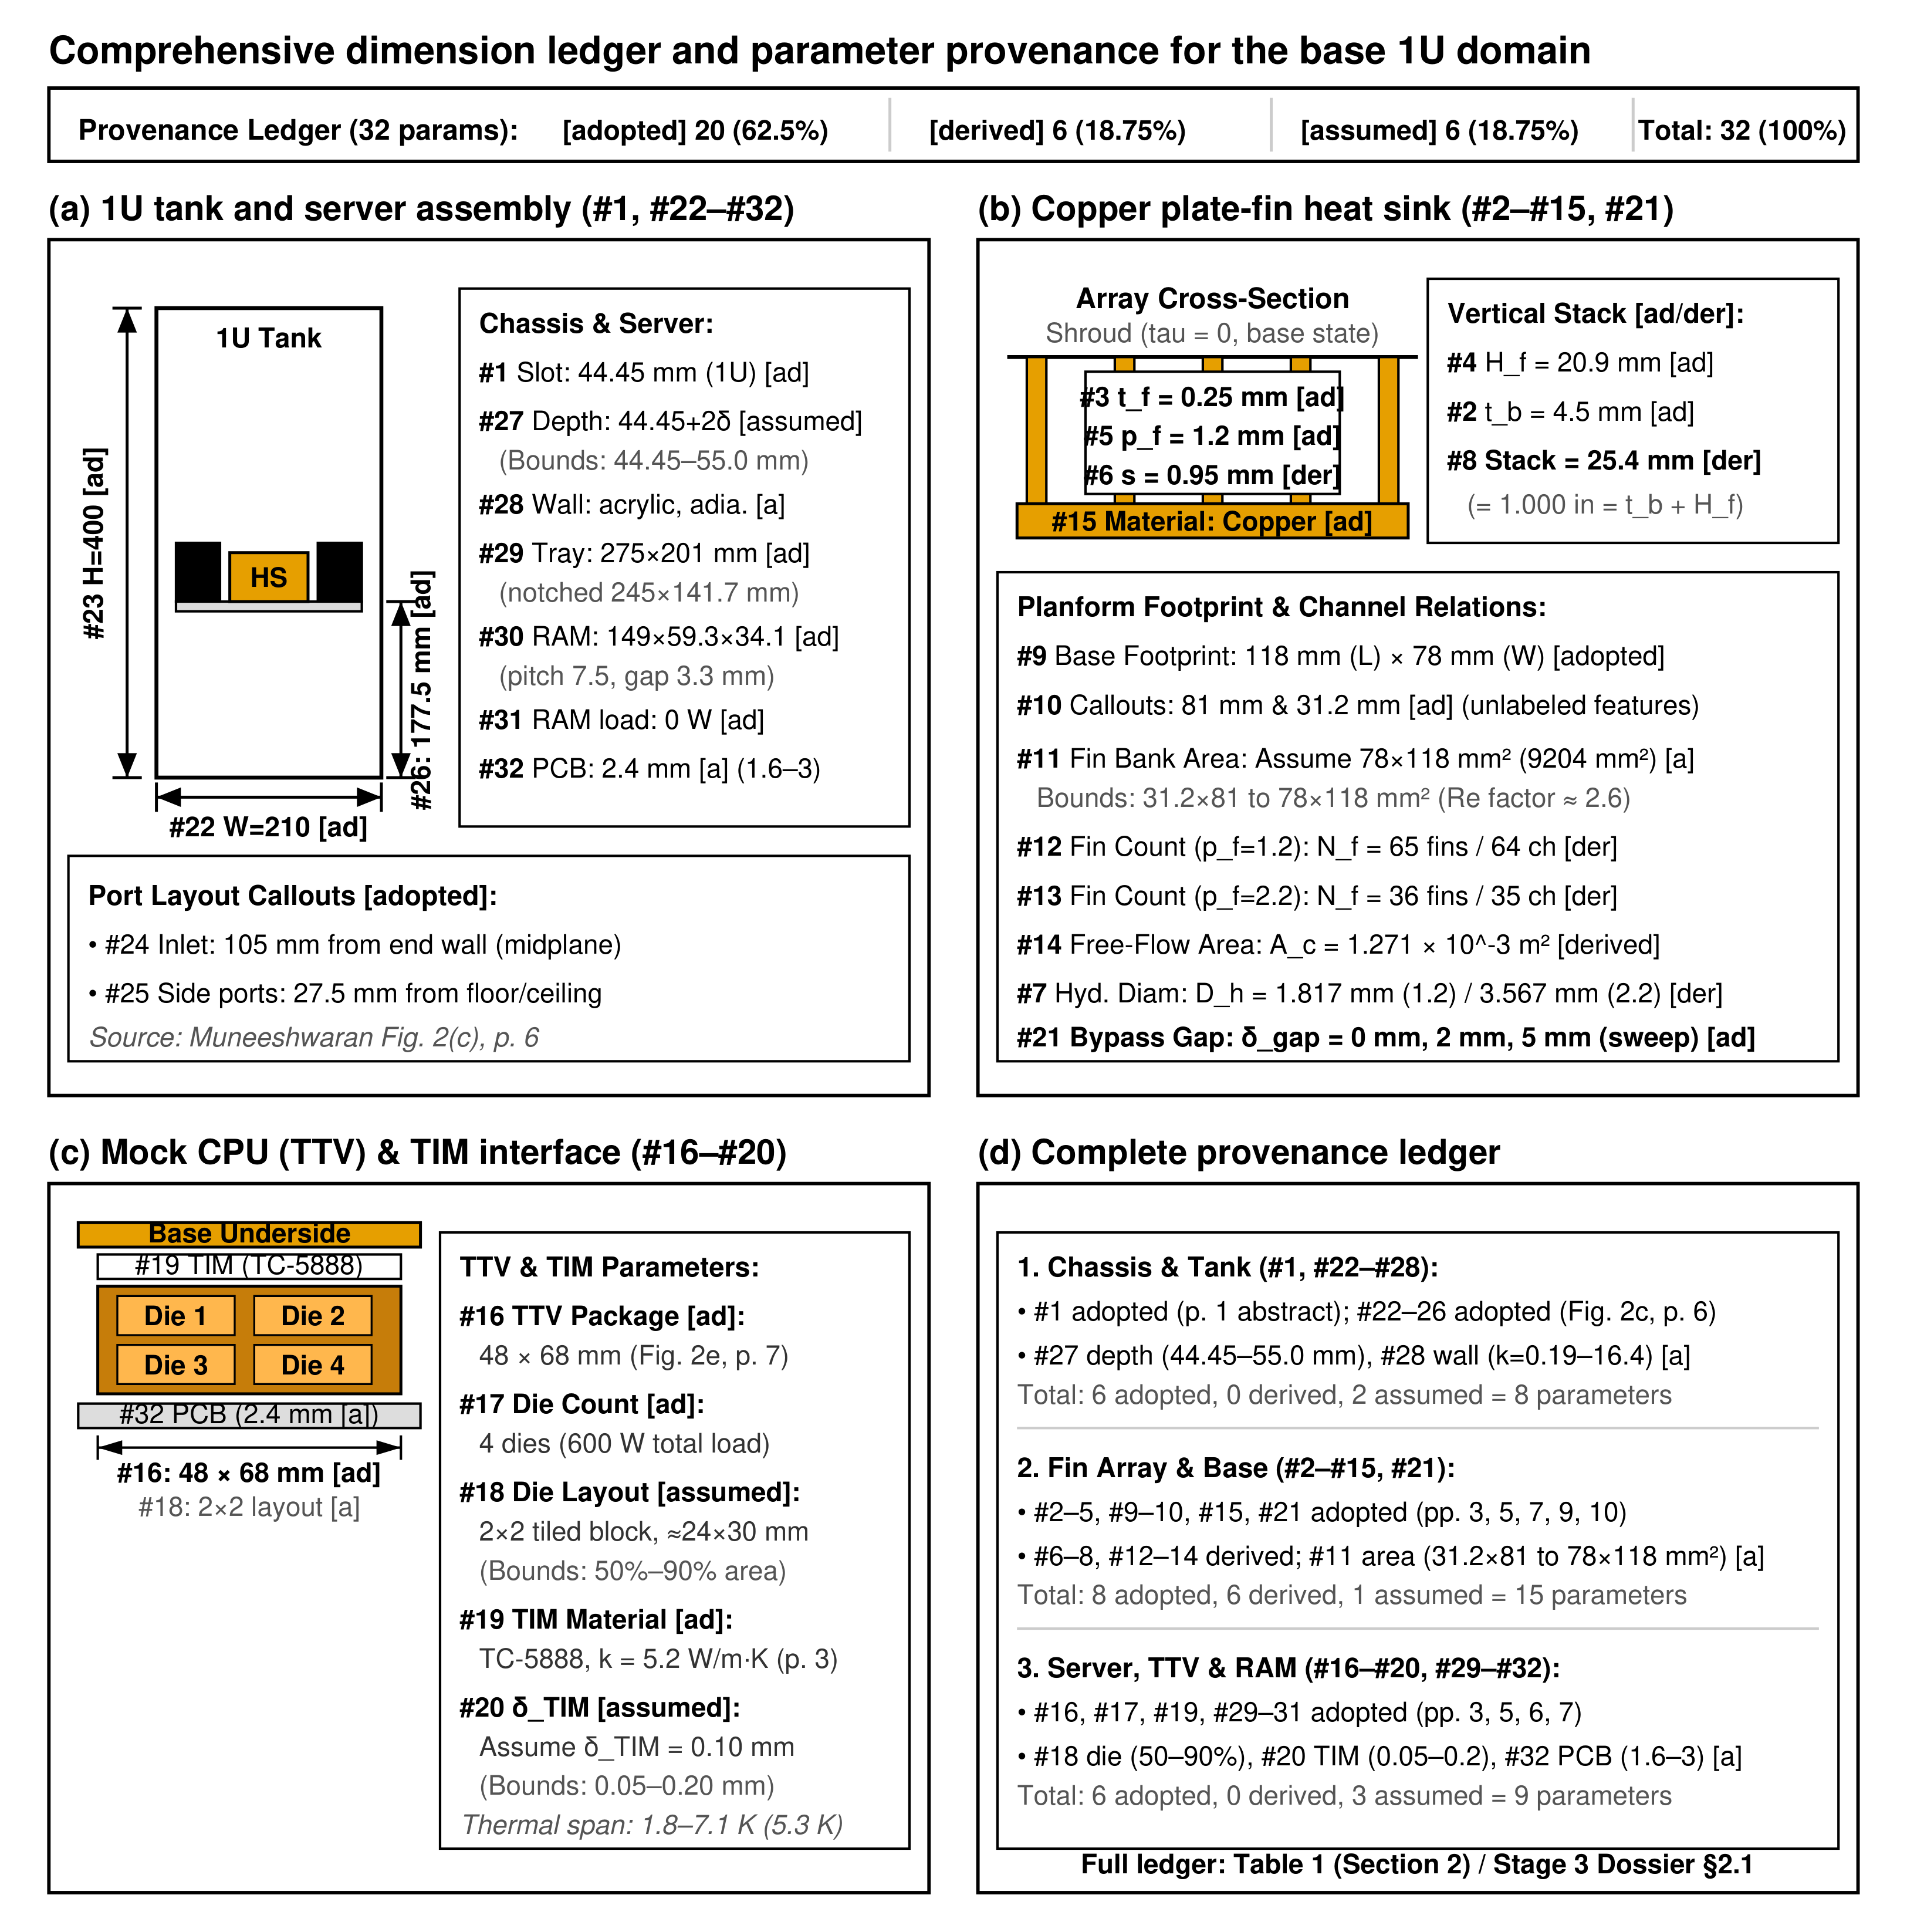
\includegraphics[width=\textwidth]{../figures/fig2_dimension_ledger.png}
\caption{Dimension ledger and parameter provenance for the base model geometry, matching
Table~\ref{tab:ledger-base}. Adopted, derived and assumed dimensions are visually distinguished
so that the source of every number in the model is visible at a glance.}
\label{fig:ledger}
\end{figure}

Two conventions follow from the ledger and are stated here so that no downstream quantity is
ambiguous. First, the fin bank is taken to span the 78~mm base width, so the span sets the channel
count and the 118~mm base length is the channel flow length. Second, the channel hydraulic
diameter of row 7 is the length scale for every Reynolds and Nusselt number reported in this
paper. That second point needs saying because the bypass and tip-clearance literature this work
builds on does not share a convention: Sastre et al.~\cite{sastre2018} use the hydraulic diameter
of the finned cross-section including the clearance slab, Mei et al.~\cite{mei2014} use the pin
diameter with the maximum velocity, Jeng~\cite{jeng2008} uses the bare rectangular duct with the
inlet velocity, Shahsavar et al.~\cite{shahsavar2021} use four times the array volume over its
wetted area, Shrigondekar et al.~\cite{shrigondekar2023} use the bare fin spacing, and Min et
al.~\cite{min2004} report no Reynolds number at all and sweep pumping power instead. Five
incompatible length scales across six papers is a large part of why no dimensionless framework for
this problem exists yet, and every literature value quoted in this paper is recomputed on the
convention above before it is compared with anything.

Applying that convention to the base geometry gives a channel Reynolds number
$\mathrm{Re}_{ch}=\dot{m}D_h/(A_c\mu)$ of roughly 5 to 122 over the 1 to 3~LPM flow range and the
15 to 35~$^{\circ}$C inlet range, if all flow is forced through the fins. The band is wide, and it
is wide for an honest reason: it carries the factor of about 2.6 between the two bounds of the
fin-bank span in row 11. No single-valued channel Reynolds number is quoted for the base geometry
anywhere in this paper. The one directly printed check available is Shrigondekar et
al.~\cite{shrigondekar2023}, who report a fin-spacing Reynolds number of about 10 to 70 for FC-40
on the same rig at the same flow rates and the same two fin pitches. Converted onto the fin-spacing
length scale, the wide-span bound of row 11 gives 2.5 to 46 and the narrow-span bound gives 6.4 to
114. The printed value therefore sits inside the narrow band and partly above the wide one, which
means this check leans against the value adopted rather than confirming it. That is recorded here
rather than smoothed over.

\subsection{Reference configuration for the anchor comparison}
\label{sec:v3}

A second, fully dimensioned geometry is carried alongside the base model so that the open-ratio
results of Chun et al.~\cite{chun2026} can be reproduced without rescaling anything.
Table~\ref{tab:ledger-v3} is its ledger. It is not a substitute for the base model and no result
from the two configurations is pooled.

\begingroup
\footnotesize
\setlength{\tabcolsep}{4pt}
\begin{longtable}{@{}l>{\raggedright\arraybackslash}p{0.225\textwidth}>{\raggedright\arraybackslash}p{0.185\textwidth}l>{\raggedright\arraybackslash}p{0.245\textwidth}@{}}
\caption{Dimension ledger for the reference configuration used in the anchor comparison, the 1U
plate-fin build of Chun et al.~\cite{chun2026}. Page numbers are the printed journal page of
\textit{Energy} \textbf{361} (2026) 141967.}
\label{tab:ledger-v3}\\
\toprule
\# & Quantity & Value & Tag & Source or arithmetic \\
\midrule
\endfirsthead
\multicolumn{5}{@{}l}{\normalfont\itshape Table~\ref{tab:ledger-v3} continued}\\
\toprule
\# & Quantity & Value & Tag & Source or arithmetic \\
\midrule
\endhead
\midrule
\multicolumn{5}{@{}r}{\normalfont\itshape continued on next page}\\
\endfoot
\bottomrule
\endlastfoot
A1  & 1U internal slot spacing        & 44.45~mm & \texttt{[adopted]} & p.~5, \S2.1 \\
A2  & Fin thickness                   & 2~mm     & \texttt{[adopted]} & Fig.~2(a), p.~5, callout under a ``Unit : mm'' header \\
A3  & Fin spacing                     & 3~mm     & \texttt{[adopted]} & Fig.~2(a), p.~5 \\
A4  & Fin height                      & 20~mm    & \texttt{[adopted]} & Fig.~2(a), p.~5 \\
A5  & Fin pitch                       & 5~mm     & \texttt{[derived]} & $2+3$ \\
A6  & Heat-sink base plate            & 72~mm width $\times$ 106~mm flow length & \texttt{[adopted]} & Fig.~2(a), p.~5 \\
A7  & Fin count                       & 15 fins, 14 channels & \texttt{[derived]} & $2N+3(N-1)=72$ gives $N=15$ exactly \\
A8  & Channel free-flow area          & $8.40\times10^{-4}$~m$^2$ & \texttt{[derived]} & $14\times3\times20$~mm$^2$ \\
A9  & Channel hydraulic diameter      & 5.217~mm & \texttt{[derived]} & $2(3)(20)/23$ \\
A10 & Copper block, mock CPU          & 50 $\times$ 65 $\times$ 8~mm & \texttt{[adopted]} & Fig.~2(a), p.~5 \\
A11 & TIM, indium foil thickness      & $\approx$0.1~mm & \texttt{[adopted]} & p.~6, \S2.1 \\
A12 & Heat-sink centre spacing on PCB & 60~mm    & \texttt{[adopted]} & p.~6, \S2.1, and Fig.~2(a), p.~5 \\
A13 & Tank internal width             & 423~mm   & \texttt{[adopted]} & Fig.~2(a), p.~5, right-hand panel headed ``Immersion tank'' \\
A14 & Tank internal height, outlet plane to distribution-plate plane & 430~mm & \texttt{[adopted]} & Fig.~2(a), p.~5, right-hand panel \\
A15 & Distribution plate, 1U build    & 10 holes, 10~mm diameter & \texttt{[adopted]} & p.~5, \S2.1 \\
A16 & Distribution plate, 3U build    & 30 holes, 5~mm diameter & \texttt{[adopted]} & p.~5, \S2.1 \\
A17 & Tank material                   & SUS304, double-layer insulation, tempered-glass window & \texttt{[adopted]} & p.~4, \S2.1; properties Table~2, p.~6 \\
A18 & Flow-control block material     & acrylic  & \texttt{[adopted]} & p.~6, \S2.1 \\
A19 & Flow-control block dimensions   & not dimensioned in the source & \texttt{[assumed]} & The open ratio is therefore defined here by the volume a block occludes, never by a block dimension \\
A20 & Tank external envelope          & not printed in the source & \texttt{[assumed]} & Not required: the computational domain is the wetted interior bounded by A13, A14 and A1 \\
A21 & Metal-foam alternative core     & 10~PPI, porosity 0.9; sweep 5 to 15~PPI, porosity 0.5 to 0.9 & \texttt{[adopted]} & p.~15 and p.~18, \S3.3 \\
\end{longtable}
\endgroup

Three specific gaps in this reference configuration are carried openly rather than closed
silently, because an independent reproducibility check found them and they are real. The source
does not print the tank's third, out-of-plane dimension, does not print the heat-sink base
thickness, and does not give the numerical inlet profile, outlet type or tank-wall thermal
condition, so the anchor comparison in Section~\ref{sec:verification} is a best-effort check
against a paper that does not fully close its own specification, not a fully reproducible
benchmark. The same three gaps are the reason A19, A20 and the base thickness never enter a
reported quantity.

\subsection{Open ratio}
\label{sec:openratio}

The bypass metric is adopted verbatim from Chun et al.~\cite{chun2026}, who introduce it as an
unnumbered display equation on their p.~11 and illustrate it in their Fig.~8. Their words for it,
quoted so that nothing is quietly reinterpreted here, are that the open ratio is
\textit{the volumetric fraction of the unobstructed fluid inlet space relative to the total heat
sink inlet volume}:

\begin{equation}
\mathrm{OR} = \frac{V_{\mathrm{open}}}{V_{\mathrm{total}}}\times 100 \quad (\%)
\label{eq:or}
\end{equation}

\noindent
Named for the geometry of Table~\ref{tab:ledger-base}, the two volumes in Eq.~(\ref{eq:or}) are
the following. $V_{\mathrm{total}}$ is the total heat-sink inlet volume, the fluid volume swept
out by the heat-sink inlet plane over the inlet-plane thickness, that is the plan area of the 1U
slot facing the heat sink multiplied by the inlet-plane thickness, spanning the full tank width
available to the flow at that height. $V_{\mathrm{open}}$ is the unobstructed fluid inlet space,
the part of $V_{\mathrm{total}}$ occupied by neither the heat sink nor a flow-control block, that
is the volume through which fluid can reach the outlets without passing between the fins. At
$\mathrm{OR}=100\%$ the tank is unobstructed and bypass is free. At $\mathrm{OR}=0\%$ every
entering parcel is directed through the heat-source region.

Three properties of the definition travel with it, because dropping any of them changes what the
number means. It is a volume ratio at the inlet plane, not an area ratio and not a clearance in
millimetres; the source never converts it to a gap width. It is geometry-specific, and the source
says so, so any open ratio quoted here travels with the geometry it was measured on. And the
blocking acts laterally, from both edges symmetrically, which in the 1U build means the top gap is
absent and the open ratio is a purely lateral quantity.

Open ratio is a geometric input. Its companion output, also taken from
Chun et al.~\cite{chun2026}, is the bypass mass fraction,

\begin{equation}
\dot{m}_{\mathrm{bypass}} = \dot{m}_{\mathrm{total}} - \dot{m}_{\mathrm{active}},
\qquad
\Phi_{\mathrm{bypass}} = \frac{\dot{m}_{\mathrm{bypass}}}{\dot{m}_{\mathrm{total}}}\times 100
\quad (\%),
\label{eq:phibypass}
\end{equation}

\noindent
where the bypass region is the flow region excluding the heat-sink passages and the region
directed toward the heat source. This paper reports $\mathrm{OR}$ as the design variable and
$\Phi_{\mathrm{bypass}}$ as the computed response, in the same pairing the source uses.

Lateral bypass and tip clearance are carried as two separate parameters and are never combined
into one scalar. The tip clearance ratio is defined as

\begin{equation}
\tau = \frac{c}{H_f},
\label{eq:tau}
\end{equation}

\noindent
the clearance height over the fin height, and is held at $\tau=0$ in the base configuration. Four
reasons keep the two apart. The 1U build that defines the open ratio has already eliminated the
top gap, so folding a tip term into it would redefine the source's own quantity while keeping its
name. No study surveyed here varies both mechanisms; every tip-clearance study varies only the tip
gap and both side-bypass studies vary only the side gap, so a combined ratio would be a quantity
with no supporting measurement anywhere. Jeng~\cite{jeng2008} argues the point directly, noting
that the tip gap dominates in magnitude and can be changed late in a design while the channel
width is fixed early by the board width, which in a 1U immersion chassis holds with extra force.
And the two responses have different shapes. Tip clearance is non-monotonic and has an interior
optimum: Min et al.~\cite{min2004} report a minimum thermal resistance of 0.058~$^{\circ}$C~W$^{-1}$
at a clearance-to-channel-width ratio of 0.6 under 2.27~W of pumping power, and Mei et
al.~\cite{mei2014} report the same competing-effects reversal. Lateral bypass is monotonic and
always detrimental, in Muneeshwaran et al.~\cite{muneeshwaran2023} across the 0 to 5~mm gap sweep
and in Chun et al.~\cite{chun2026} across the open-ratio sweep. Collapsing a bounded parameter
with an optimum and a monotone detrimental one into a single scalar would make any interior
optimum in the combined ratio unattributable to either mechanism. Sastre et al.~\cite{sastre2018}
supply the warning empirically: even one clearance parameter was strong enough to split their
Nusselt-Graetz curves into separate families rather than one fit.

One out-of-sample check on the open ratio exists and is used. Jeng~\cite{jeng2008} parameterises
lateral bypass around a square pin-fin sink as the ratio $W/L$ of channel width to sink length. For
a constant-height inlet plane the two parameterisations map exactly, $\mathrm{OR} = (1-L/W)\times
100$, so $W/L$ of 1, 2, 3 and 5 correspond to open ratios of 0, 50, 66.7 and 80\%. Jeng's
recommendation of $W/L$ between 2 and 3 therefore sits inside the range swept here, in a different
fluid and a different fin type. The mapping is derived here, not printed in either source, and it
holds only when the open volume is the lateral space at the same inlet-plane height.

\subsection{Working fluids and thermophysical properties}
\label{sec:properties}

Two dielectric coolants are used. FC-40, a perfluorinated fluorocarbon, is the primary fluid: it is
the one coolant for which more than one independent group in this literature has published usable
property data, so a property error can be caught by cross-checking rather than trusted. GC-5X, an
oil-based dielectric, is the high-viscosity contrast case. Carrying two fluids is not decoration.
Chun et al.~\cite{chun2026} show that open-ratio sensitivity is a strong function of viscosity,
with thermal resistance falling 6.1\% for FC-40 but 45.6\% for GC-5X as the bypass is closed, so a
framework claimed to be dimensionless must be exercised across more than one Prandtl decade or the
claim is untested.

Table~\ref{tab:fluidprops} gives the property treatment and the source of every value.

\begin{table}[htbp]
\centering
\caption{Coolant thermophysical properties and their sources. The correlations of Chun et
al.~\cite{chun2026} take $T$ in kelvin; see the discussion below.}
\label{tab:fluidprops}
\footnotesize
\setlength{\tabcolsep}{4pt}
\begin{tabular}{@{}l>{\raggedright\arraybackslash}p{0.105\textwidth}>{\raggedright\arraybackslash}p{0.405\textwidth}>{\raggedright\arraybackslash}p{0.215\textwidth}@{}}
\toprule
Fluid & Property & Value or correlation ($T$ in K) & Source \\
\midrule
FC-40 & $\rho$    & $2499 - 2.16\,T$~kg~m$^{-3}$ & \cite{chun2026}, Table~3, p.~7 \\
FC-40 & $k$       & $0.086 - 6.90\times10^{-5}\,T$~W~m$^{-1}$~K$^{-1}$ & \cite{chun2026}, Table~3, p.~7 \\
FC-40 & $c_p$     & $590 + 1.55\,T$~J~kg$^{-1}$~K$^{-1}$ & \cite{chun2026}, Table~3, p.~7 \\
FC-40 & $\mu$     & $0.0429 - 0.162\times10^{-3}\,T$ $+\;1.08\times10^{-7}\,T^2$~Pa~s & \cite{chun2026}, Table~3, p.~7 \\
FC-40 & $\rho$ & 1874.44~kg~m$^{-3}$ at 16~$^{\circ}$C & \cite{muneeshwaran2023}, Table~4, p.~7 \\
FC-40 & $\nu$ & $5\times10^{-6}$, $1.5\times10^{-6}$, $5.4\times10^{-7}$~m$^2$~s$^{-1}$ at 0, 40, 100~$^{\circ}$C & \cite{muneeshwaran2023}, Table~4, p.~7 \\
FC-40 & $c_p$ & 1014, 1076, 1169.4~J~kg$^{-1}$~K$^{-1}$ at 0, 40, 100~$^{\circ}$C & \cite{muneeshwaran2023}, Table~4, p.~7 \\
FC-40 & $k$ & 0.067, 0.0642, 0.0601~W~m$^{-1}$~K$^{-1}$ at 0, 40, 100~$^{\circ}$C & \cite{muneeshwaran2023}, Table~4, p.~7 \\
FC-40 & $\beta$   & $1.2\times10^{-3}$~K$^{-1}$ & \cite{muneeshwaran2023}, Table~4, p.~7 \\
FC-40 & Boiling pt. & 165~$^{\circ}$C at 1~bar & \cite{muneeshwaran2023}, Table~4, p.~7 \\
FC-40 & $\mathrm{Pr}$ & 67.5 at 25~$^{\circ}$C & \texttt{[derived]} from the correlations above \\
\midrule
GC-5X & $\rho$    & $1049.862 - 0.75\,T$~kg~m$^{-3}$ & \cite{chun2026}, Table~3, p.~7 \\
GC-5X & $k$       & $0.199367 - 1.8\times10^{-4}\,T$~W~m$^{-1}$~K$^{-1}$ & \cite{chun2026}, Table~3, p.~7 \\
GC-5X & $c_p$     & $2076.055 + 0.3\,T$~J~kg$^{-1}$~K$^{-1}$ & \cite{chun2026}, Table~3, p.~7 \\
GC-5X & $\mu$     & $0.6449 - 4.1234\times10^{-3}\,T$ $+\;8.9697\times10^{-6}\,T^2$ $-\;6.5833\times10^{-9}\,T^3$~Pa~s & \cite{chun2026}, Table~3, p.~7 \\
GC-5X & $\beta$   & $9.08\times10^{-4}$~K$^{-1}$ at 25~$^{\circ}$C & \texttt{[derived]}, $\beta=-\rho^{-1}\partial\rho/\partial T$ on the density fit of this table. No measured value is printed in any source consulted \\
GC-5X & $\mathrm{Pr}$ & 570 at 25~$^{\circ}$C & \texttt{[derived]} from the correlations above \\
\bottomrule
\end{tabular}
\end{table}

Two findings about these properties came out of checking them rather than copying them, and both
change how the correlations may be used.

The first is that the correlations of Chun et al.~\cite{chun2026} take $T$ in kelvin, which their
paper does not state and their own nomenclature contradicts by defining $T$ in degrees Celsius.
The evidence is arithmetic and it is decisive. With $T$ in kelvin the FC-40 density fit returns
1874.4~kg~m$^{-3}$ at 289.15~K, against the 1874.44~kg~m$^{-3}$ at 16~$^{\circ}$C measured
independently by Muneeshwaran et al.~\cite{muneeshwaran2023}. The conductivity fit returns 0.0672,
0.0644 and 0.0603~W~m$^{-1}$~K$^{-1}$ at 0, 40 and 100~$^{\circ}$C against their printed 0.067,
0.0642 and 0.0601, and the specific-heat fit returns 1013.4, 1075.4 and 1168.4~J~kg$^{-1}$~K$^{-1}$
against their printed 1014, 1076 and 1169.4. Three properties agree to better than 0.1\% at three
temperatures each on one unit convention and are irreconcilable on the other. The same conclusion
follows independently from the source's own mass-flow table, which converts to exactly 5.00~LPM per
heat sink at the stated 10~LPM for two heat sinks only when the density is evaluated in kelvin.
This is an inference from the paper's numbers, not a printed statement, and it should be confirmed
with the corresponding author before any anchor result is reproduced.

The second finding is a limit on the FC-40 viscosity fit, and it constrains the model. That
quadratic reaches zero at about 343~K, or 70~$^{\circ}$C, and is negative above it, so it cannot be
used at wall temperatures approaching the 80~$^{\circ}$C case-temperature limit of the base
paper~\cite{muneeshwaran2023}. Within its useful band it is good: against the kinematic-viscosity
points of Muneeshwaran et al.\ interpolated logarithmically it agrees to 1.2\% at 35~$^{\circ}$C
and 3.9\% at 25~$^{\circ}$C, degrading to 13\% at 15~$^{\circ}$C and 30\% at 0~$^{\circ}$C. FC-40
viscosity is therefore evaluated from the fit between 20 and 60~$^{\circ}$C and from the measured
points of Muneeshwaran et al.\ outside that band. The GC-5X cubic stays positive and monotone
across the whole range of interest and needs no such restriction.

Solid properties are listed in Table~\ref{tab:solidprops}. Where two sources print a value, both
are named, and where they agree exactly that is said, because agreement between independently
published tables is the only property check available in the absence of a measurement of our own.

\begin{table}[htbp]
\centering
\caption{Solid domain properties and their sources. Density in kg~m$^{-3}$, specific heat in J~kg$^{-1}$~K$^{-1}$, thermal conductivity in W~m$^{-1}$~K$^{-1}$.}
\label{tab:solidprops}
\footnotesize
\setlength{\tabcolsep}{4pt}
\begin{tabular}{@{}>{\raggedright\arraybackslash}p{0.155\textwidth}cc>{\raggedright\arraybackslash}p{0.105\textwidth}>{\raggedright\arraybackslash}p{0.30\textwidth}@{}}
\toprule
Domain & $\rho$ & $c_p$ & $k$ & Source \\
\midrule
Copper, fins and base & 8978 & 381 & 387.6 & \cite{chun2026}, Table~2, p.~6; the identical triplet is printed independently in \cite{khoshvaghtaliabadi2026oblique}, Table~1, p.~5 \\
TIM, base model, thermal grease & \multicolumn{2}{c}{not printed} & 5.2 & \cite{muneeshwaran2023}, p.~3, \S2.1 \\
TIM, reference configuration, indium & 7310 & 234 & 81.8 & \cite{chun2026}, Table~2, p.~6 \\
PCB substrate & 1850 & 1000 & 0.3 & \cite{khoshvaghtaliabadi2026oblique}, Table~1, p.~5 \\
PCB substrate, alternative & 3600 & 720 & 42.0 in-plane, 0.5 cross-plane & \cite{chun2026}, Table~2, p.~6 \\
SUS304, reference configuration tank & 8000 & 500 & 16.4 & \cite{chun2026}, Table~2, p.~6 \\
Acrylic, flow-control block and tank wall & 1180 & 1460 & 0.21 & \cite{chun2026}, Table~2, p.~6 \\
\bottomrule
\end{tabular}
\end{table}

The two PCB entries disagree by two orders of magnitude in conductivity because they describe
different things: one is an isotropic bulk laminate value, the other resolves the copper-plane
anisotropy. The isotropic entry is used for the base model, where the board is an unloaded
conduction path, and the anisotropic entry is used for the anchor comparison so that the
reference configuration keeps its own source's convention. Neither value moves a reported quantity
in this work, since the board carries no thermal load in the base model. All solid property values
in Table~\ref{tab:solidprops} are attributed within their source to further references rather than
measured there, and are carried on that basis.

\subsection{Assumptions}
\label{sec:assumptions}

Eight quantities in Tables~\ref{tab:ledger-base} and \ref{tab:ledger-v3} are not available in any
source consulted. Each is listed below with the value taken, the reason, the defensible bounds and
the results it can move. Nothing here is assumed because it was convenient, and nothing that a
result depends on is hidden inside a sentence.

\noindent\textbf{Fin-bank plan area, 78~mm $\times$ 118~mm (row 11).}\ The base outline of the heat sink is
dimensioned but the drawing does not label which feature its two interior callouts, 81~mm and
31.2~mm, terminate on. Bounds are therefore 31.2 $\times$ 81~mm at the low end and 78 $\times$
118~mm at the high end, a factor of 3.6 in plan area. The wide value is taken because it is the
only one under which the 48 $\times$ 68~mm mock-processor footprint of row 16 is fully covered by
the fin array. The counter-evidence is stated in Section~\ref{sec:geometry} and is not resolved:
converting the printed fin-spacing Reynolds range of Shrigondekar et al.~\cite{shrigondekar2023}
onto this geometry leans toward the narrow bound. Results moved: the span sets the channel count,
64 channels at 78~mm against 25 at 31.2~mm, hence a free-flow area of 1271~mm$^2$ against
496~mm$^2$, a factor of about 2.6 on channel velocity and on channel Reynolds number. Every
Reynolds number quoted for the base model carries that factor as a band. Thermal resistance is far
less sensitive, since the area enters through fin efficiency and total wetted area rather than
linearly. This is the largest single geometric uncertainty in the model, and the cheapest way to
settle it is a higher-resolution copy of the source drawing or a question to its corresponding
author.

\noindent\textbf{Die partition inside the mock-processor package (row 18).}\ The four dies are drawn as a
tiled block but the block is not dimensioned. Bounds are a die block between 50\% and 90\% of the
48 $\times$ 68~mm package footprint. The assumption is low-risk because the heat load is applied as
a boundary condition at the heat-sink base, following the base paper's own numerical
treatment~\cite{muneeshwaran2023}, so the die partition never enters the model. Results moved: only
a local peak junction temperature post-process, which this paper does not report.

\noindent\textbf{TIM bond-line thickness, 0.10~mm (row 20).}\ The base paper names the grease and gives its
conductivity but not the bond line. The value is set to match the indium-foil thickness printed for
the reference configuration~\cite{chun2026} so that both configurations share one interface
convention. Bounds 0.05 to 0.20~mm, the usual range for a screwed-down grease line. Results moved:
absolute case temperature shifts by about 5.3~K across those bounds ($-1.8$~K to $+3.5$~K relative to
the 0.10~mm nominal) at 600~W over the row 16 footprint. Thermal-resistance differences between open
ratios are insensitive to it, because it is a series resistance common to every case.

\noindent\textbf{Tank depth, 44.45~mm internal plus twice the bypass gap (row 27).}\ Genuinely absent. The tank
drawing carries no callout for the out-of-plane thickness and the body text gives none. The value
is chosen so that the tank interior is exactly the 1U slot the source's own abstract specifies.
Bounds 44.45 to 55~mm internal. Results moved: this dimension sets the bypass area and therefore
is the open ratio. It is the most consequential assumption in the ledger, and it is precisely why
this paper parameterises on the dimensionless open ratio rather than on an absolute tank depth.

\noindent\textbf{Tank wall material and outer boundary (row 28).}\ The base paper never names the tank material.
Acrylic with $k = 0.19$~W~m$^{-1}$~K$^{-1}$ is taken, consistent with the transparent wall in the
source's own photograph, with an adiabatic outer face. Bounds on $k$ run from 0.19 for acrylic to
16.4~W~m$^{-1}$~K$^{-1}$ for the stainless steel used in the reference
configuration~\cite{chun2026}. Results moved: none of those reported. The adiabatic outer face is
the source's own stated condition, since it reports that the entire experimental system was
insulated and that the heat loss was negligible~\cite{muneeshwaran2023}.

\noindent\textbf{PCB thickness, 2.4~mm (row 32).}\ Not given by the base paper. Taken from the only printed
PCB thickness available for a 1U immersion server~\cite{khoshvaghtaliabadi2026oblique}. Bounds 1.6
to 3.0~mm. Results moved: none reported here; the board is an unloaded conduction path of
$k \approx 0.3$~W~m$^{-1}$~K$^{-1}$.

\noindent\textbf{Flow-control block dimensions in the reference configuration (row A19).}\ The blocks are shown
schematically in the source but given no size. The open ratio is therefore defined by the volume a
block occludes, as in Eq.~(\ref{eq:or}), never by a block dimension. Results moved: the mapping
from open ratio to bypass fraction. Since this paper reports the open ratio as an input and the
bypass fraction as a computed output, no reported quantity requires the block geometry.

\noindent\textbf{External tank envelope in the reference configuration (row A20).}\ Not printed. Not required,
because the computational domain is the wetted interior bounded by rows A13, A14 and A1.

A separate set of quantities is held fixed rather than assumed, and each is fixed for a stated
reason. The rack unit height is held at 44.45~mm because it is an industry dimensional standard
printed identically by three independent groups~\cite{muneeshwaran2023,chun2026,kim2025}; it is not
a free design variable, and Kim et al.\ already swept it from 0.8U to 1.2U if a sensitivity
precedent is wanted. The mock-processor footprint is held at 48 $\times$ 68~mm because fixing the
heat-source footprint is what makes the open ratio the only varying geometric quantity; if the
footprint moved, a change in thermal resistance could not be attributed to bypass. The heat-sink
base thickness is held at 4.5~mm because it sets spreading resistance, which sits in series with
the convective resistance the open ratio acts on, so holding it keeps the two separable. The fin
material is held at copper: with a solid-to-fluid conductivity ratio near 6000 for FC-40, fin
efficiency is near unity and the result is insensitive to the copper grade, whereas switching to
aluminium would change fin efficiency and confound the bypass conclusion. The port arrangement is
held at the T-configuration because the base paper shows it is a first-order effect, 12.6\% in
thermal resistance against the Z-configuration, and because under the Z-configuration most of the
fluid bypasses the heat sink anyway; holding it removes a competing bypass mechanism so that the
open ratio is the only one varied~\cite{muneeshwaran2023}.

Fin pitch is deliberately not held constant. It is a second factor at the two printed levels of
1.2 and 2.2~mm, because the pitch and bypass interact: the penalty for opening the gap from 0 to
5~mm is 3\% at the coarse pitch but 7.4\% at the fine one~\cite{muneeshwaran2023}. The coolant is
deliberately not held constant either, for the Prandtl-range reason given in
Section~\ref{sec:properties}.
.
%
% PACKAGES REQUIRED IN main.tex PREAMBLE (not currently present):
%   \usepackage{booktabs}
%   \usepackage{array}      (for the >{\raggedright\arraybackslash}p{} column type)
% =============================================================================

\section{Problem formulation}
\label{sec:formulation}

\subsection{Base geometry}
\label{sec:geometry}

The model geometry is the 1U immersion server of Muneeshwaran et al.~\cite{muneeshwaran2023}:
a copper plate-fin heat sink clamped to a four-die thermal test vehicle on a printed circuit
board, with a bank of non-dissipating memory modules alongside it, the whole tray submerged in a
sealed 1U tank. Coolant enters through a port on the tank floor directly beneath the heat sink
and leaves through two ports at the top of the opposite faces, the arrangement those authors call
the T-configuration. That choice of base is not a matter of taste. It is the only 1U immersion
architecture in the surveyed literature whose server tray, heat sink, tank, memory bank and mock
processor all carry printed dimension callouts, so the domain can be rebuilt without scaling
anything off a figure. It is also the architecture that Chun et al.~\cite{chun2026} identify as
prior bypass-control work, that B. Zhang et al.~\cite{zhang2026} state they reconstructed as their
own computational domain, that Khoshvaght-Aliabadi and co-workers rebuilt twice as a validation
replica~\cite{khoshvaghtaliabadi2026oblique,khoshvaghtaliabadi2026component}, and from which Kim
et al.~\cite{kim2025} took their inlet and outlet arrangement. Only the first of those four is a
reuse of the architecture as a study domain; the others are weaker forms of reliance and are
described here as such.

The bypass mechanism this paper is about is present in the base paper and was measured there.
Muneeshwaran et al.~\cite{muneeshwaran2023} swept the clearance between the heat sink and the 1U
tank inner wall at 5, 2 and 0~mm, reported a 3\% to 7.4\% rise in thermal resistance and a
0.7~$^{\circ}$C to 1.5~$^{\circ}$C rise in case temperature as the gap opened, and adopted the
no-gap build for everything that followed. Their flow visualisation shows the reason: fluid takes
the clearance because its hydraulic resistance is lower, and that stream does no useful heat
transfer. The open ratio of Section~\ref{sec:openratio} is the dimensionless generalisation of
exactly this clearance.

\begin{figure}[htbp]
\centering
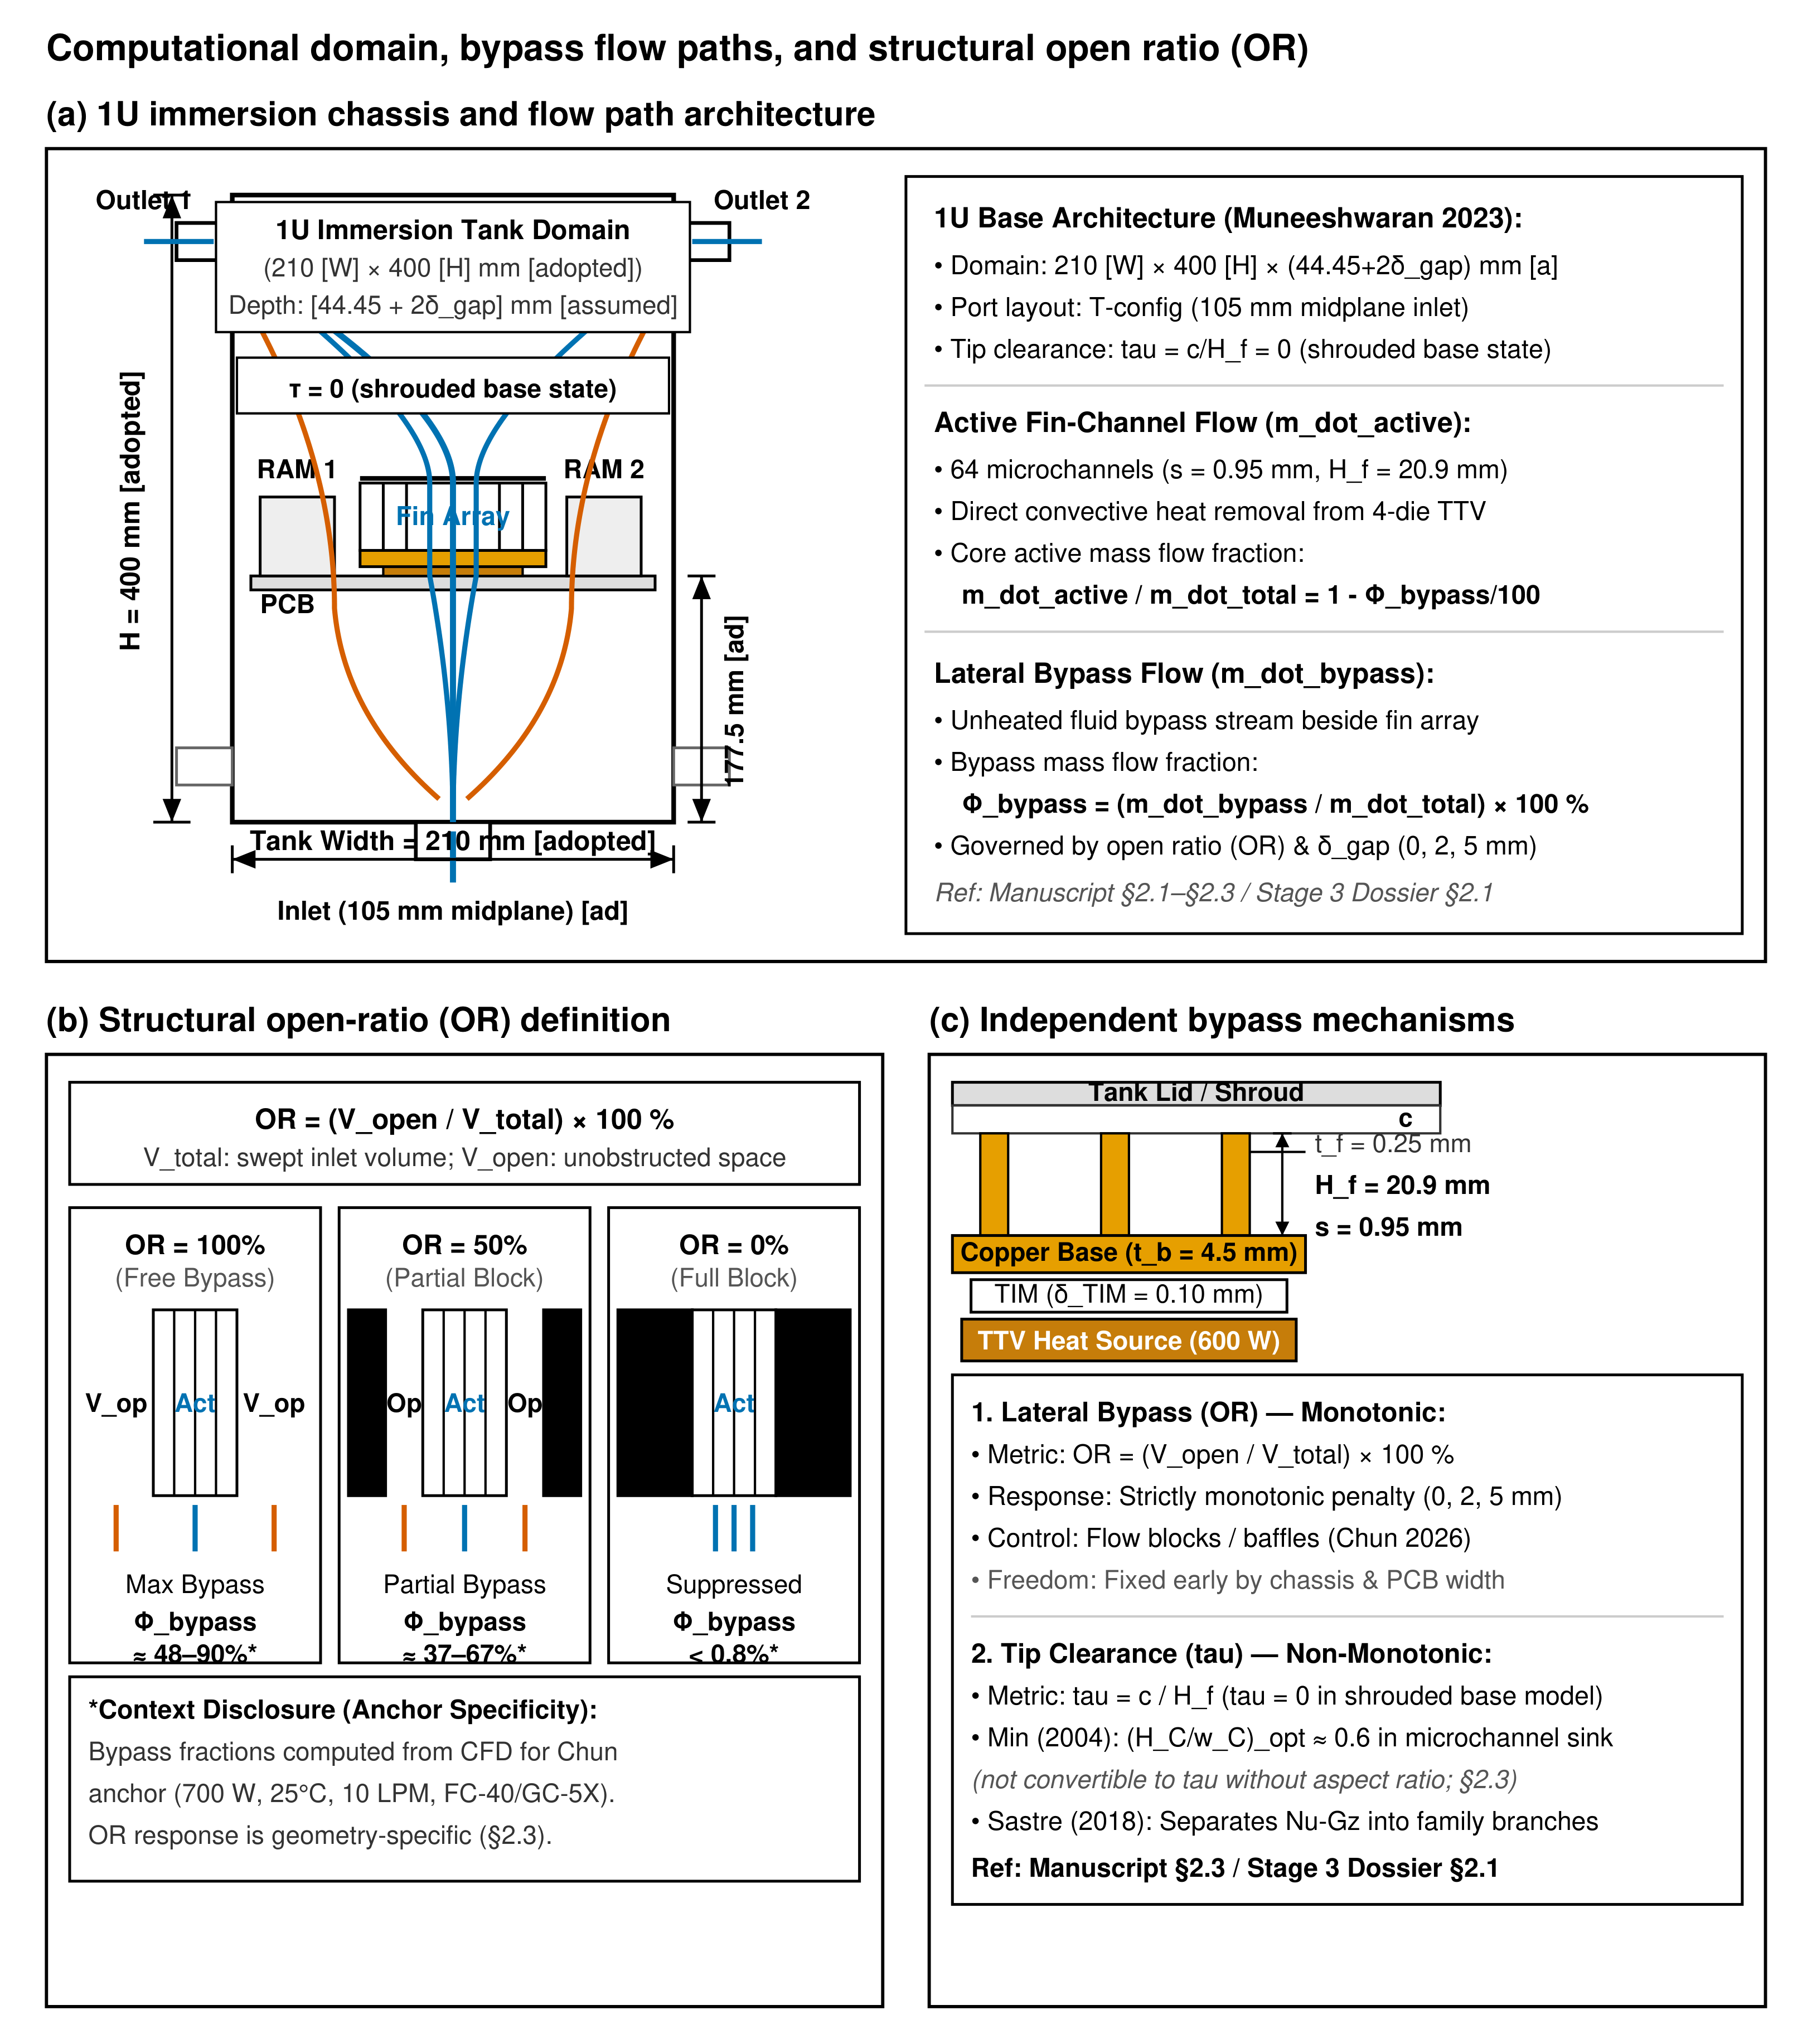
\includegraphics[width=\textwidth]{../figures/fig1_domain.png}
\caption{Computational domain, bypass flow paths and the open-ratio definition. (a) the 1U
immersion chassis with the active fin-channel flow and lateral bypass stream (with the shrouded
$\tau=0$ base state and independent tip clearance treated in panel (c)). (b) the open-ratio
definition at the heat-sink inlet plane across three blockage states. (c) lateral bypass and tip
clearance shown as the two independent mechanisms carried separately in this model, per
Section~\ref{sec:openratio}.}
\label{fig:domain}
\end{figure}

Table~\ref{tab:ledger-base} is the complete dimension ledger for the base model. Every row carries
one of three tags. A row tagged \texttt{[adopted]} is printed in the cited source at the cited
page, in body text, in a table, or as a dimension callout drawn on a figure. A row tagged
\texttt{[derived]} is computed from \texttt{[adopted]} rows, with the arithmetic shown. A row
tagged \texttt{[assumed]} is not available in any source consulted, and its value, its bounds and
the results it can move are stated in Section~\ref{sec:assumptions}. No row in the ledger is
digitised from a plot. Several of the \texttt{[adopted]} rows are recoverable only by rendering
the source page to an image and reading the drawing, because plain text extraction drops
dimension callouts that exist as vector labels inside a figure; those rows name the figure.

\begingroup
\footnotesize
\setlength{\tabcolsep}{4pt}
\begin{longtable}{@{}r>{\raggedright\arraybackslash}p{0.200\textwidth}c>{\raggedright\arraybackslash}p{0.135\textwidth}l>{\raggedright\arraybackslash}p{0.275\textwidth}@{}}
\caption{Dimension ledger for the base model, the 1U immersion server of Muneeshwaran et
al.~\cite{muneeshwaran2023}. Page numbers are the printed journal page of
\textit{Int.\ Commun.\ Heat Mass Transf.} \textbf{145} (2023) 106843, which coincides with the
PDF page index for this article.}
\label{tab:ledger-base}\\
\toprule
\# & Quantity & Symbol & Value & Tag & Source or arithmetic \\
\midrule
\endfirsthead
\multicolumn{6}{@{}l}{\normalfont\itshape Table~\ref{tab:ledger-base} continued}\\
\toprule
\# & Quantity & Symbol & Value & Tag & Source or arithmetic \\
\midrule
\endhead
\midrule
\multicolumn{6}{@{}r}{\normalfont\itshape continued on next page}\\
\endfoot
\bottomrule
\endlastfoot
1  & Rack unit height, server slot        &            & 44.45~mm & \texttt{[adopted]} & p.~1, abstract \\
2  & Heat-sink base thickness             & $t_b$      & 4.5~mm   & \texttt{[adopted]} & p.~3, \S2.1 \\
3  & Fin thickness                        & $t_f$      & 0.25~mm  & \texttt{[adopted]} & p.~3, \S2.1 \\
4  & Fin height                           & $H_f$      & 20.9~mm  & \texttt{[adopted]} & p.~3, \S2.1 \\
5  & Fin pitch, two builds                & $p_f$      & 1.2 and 2.2~mm & \texttt{[adopted]} & p.~3; Table~3, p.~7 \\
6  & Fin channel width                    & $s$        & 0.95~mm; 1.95~mm & \texttt{[derived]} & $s=p_f-t_f$ \\
7  & Channel hydraulic diameter           & $D_h$      & 1.817~mm; 3.567~mm & \texttt{[derived]} & $D_h=2sH_f/(s+H_f)$ \\
8  & Heat-sink stack height               & $t_b+H_f$  & 25.4~mm  & \texttt{[derived]} & $4.5+20.9$ \\
9  & Heat-sink base footprint             & $L\times W$& 118~mm $\times$ 78~mm & \texttt{[adopted]} & Fig.~2(b), p.~5, rendered callouts \\
10 & Raised finned-section callouts       &            & 81~mm and 31.2~mm & \texttt{[adopted]} & Fig.~2(b), p.~5. The drawing does not label which feature each callout terminates on \\
11 & Fin-bank plan area                   & $A_{bank}$ & 78~mm $\times$ 118~mm & \texttt{[assumed]} & Bounds 31.2 $\times$ 81~mm to 78 $\times$ 118~mm; see Section~\ref{sec:assumptions} \\
12 & Fin count, $p_f=1.2$~mm              & $N_f$      & 65 fins, 64 channels & \texttt{[derived]} & $Nt_f+(N-1)s=W$ on row 11 \\
13 & Fin count, $p_f=2.2$~mm              & $N_f$      & 36 fins, 35 channels & \texttt{[derived]} & same relation on row 11 \\
14 & Channel free-flow area, base build   & $A_c$      & $1.271\times10^{-3}$~m$^2$ & \texttt{[derived]} & $64\times0.95\times20.9$~mm$^2$ \\
15 & Heat-sink material                   &            & copper   & \texttt{[adopted]} & p.~3, \S2.1 \\
16 & Mock CPU package footprint           &            & 48~mm $\times$ 68~mm & \texttt{[adopted]} & Fig.~2(e), p.~7, rendered callouts \\
17 & Die count                            &            & 4, independently modulated & \texttt{[adopted]} & p.~3, \S2.1; Fig.~2(e), p.~7 \\
18 & Individual die footprint             &            & 2 $\times$ 2 tiling of a centred block & \texttt{[assumed]} & Bounds 50\% to 90\% of the package footprint; see Section~\ref{sec:assumptions} \\
19 & Thermal interface material           &            & grease TC-5888, $k=5.2$ &  \texttt{[adopted]} & p.~3, \S2.1; $k$ in W~m$^{-1}$~K$^{-1}$ \\
20 & TIM bond-line thickness              & $\delta_{TIM}$ & 0.10~mm & \texttt{[assumed]} & Bounds 0.05 to 0.20~mm; see Section~\ref{sec:assumptions} \\
21 & Bypass gap, heat sink to tank wall   & $\delta_{gap}$ & 0, 2, 5~mm & \texttt{[adopted]} & p.~5, \S3.2; Fig.~6, p.~9; Fig.~7, p.~10 \\
22 & Tank, long horizontal dimension      &            & 210~mm   & \texttt{[adopted]} & Fig.~2(c), p.~6, rendered callouts \\
23 & Tank, vertical dimension             &            & 400~mm   & \texttt{[adopted]} & Fig.~2(c), p.~6 \\
24 & Bottom inlet axis from tank end wall &            & 105~mm   & \texttt{[adopted]} & Fig.~2(c), p.~6; $105=210/2$, so the inlet is on the tank mid-plane \\
25 & Side port axes from floor and ceiling&            & 27.5~mm  & \texttt{[adopted]} & Fig.~2(c), p.~6 \\
26 & Heat-sink underside above tank floor &            & 177.5~mm & \texttt{[adopted]} & Fig.~2(c), p.~6 \\
27 & Tank depth, out-of-plane             &            & 44.45~mm internal $+\,2\delta_{gap}$ & \texttt{[assumed]} & Bounds 44.45 to 55~mm internal; see Section~\ref{sec:assumptions} \\
28 & Tank wall material                   &            & acrylic, adiabatic outer face & \texttt{[assumed]} & $k=0.19$; bounds 0.19 to 16.4~W~m$^{-1}$~K$^{-1}$; see Section~\ref{sec:assumptions} \\
29 & Server tray outline                  &            & 275 and 245~mm; 201 and 141.7~mm & \texttt{[adopted]} & Fig.~2(a), p.~5, rendered callouts \\
30 & Memory bank envelope                 &            & 149 $\times$ 59.3 $\times$ 34.1~mm; pitch 7.5~mm; gap 3.3~mm & \texttt{[adopted]} & Fig.~2(d), p.~6, rendered callouts \\
31 & Memory thermal load                  &            & zero, flow obstruction only & \texttt{[adopted]} & p.~3, \S2.1 \\
32 & PCB thickness                        &            & 2.4~mm   & \texttt{[assumed]} & From Khoshvaght-Aliabadi et al.~\cite{khoshvaghtaliabadi2026oblique}, Table~1, p.~5; bounds 1.6 to 3.0~mm \\
\end{longtable}
\endgroup

\begin{figure}[htbp]
\centering
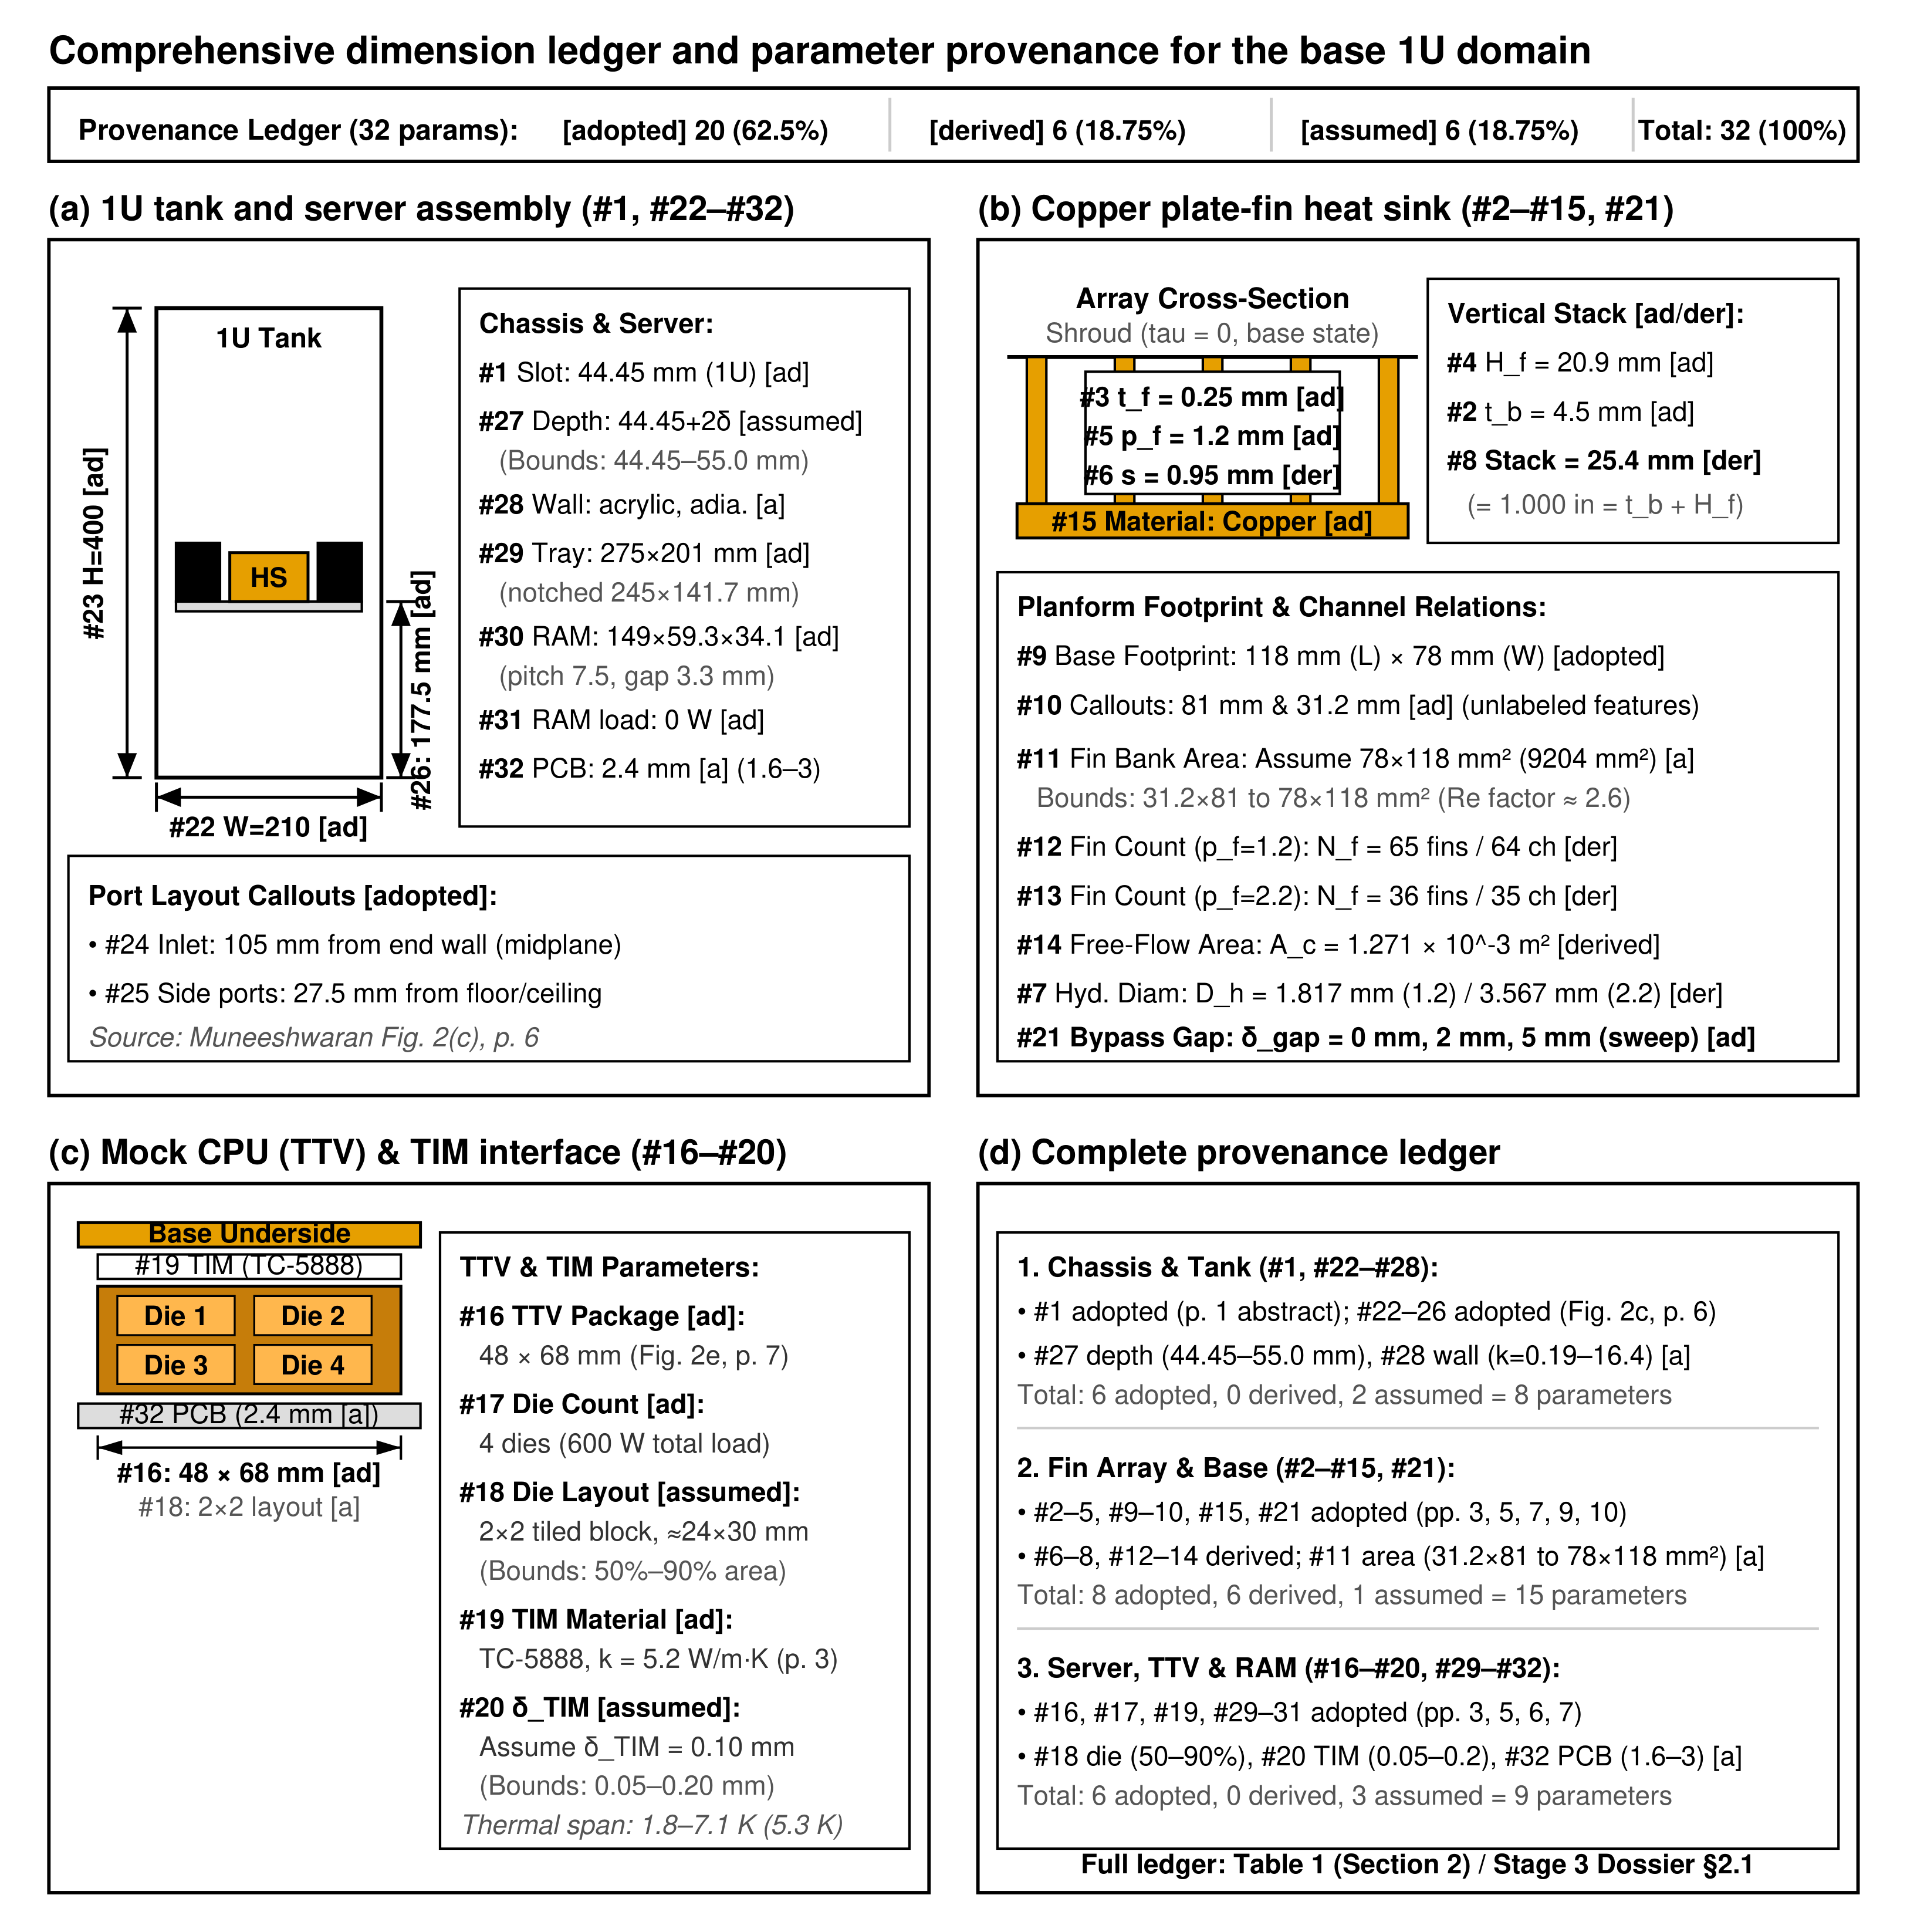
\includegraphics[width=\textwidth]{../figures/fig2_dimension_ledger.png}
\caption{Dimension ledger and parameter provenance for the base model geometry, matching
Table~\ref{tab:ledger-base}. Adopted, derived and assumed dimensions are visually distinguished
so that the source of every number in the model is visible at a glance.}
\label{fig:ledger}
\end{figure}

Two conventions follow from the ledger and are stated here so that no downstream quantity is
ambiguous. First, the fin bank is taken to span the 78~mm base width, so the span sets the channel
count and the 118~mm base length is the channel flow length. Second, the channel hydraulic
diameter of row 7 is the length scale for every Reynolds and Nusselt number reported in this
paper. That second point needs saying because the bypass and tip-clearance literature this work
builds on does not share a convention: Sastre et al.~\cite{sastre2018} use the hydraulic diameter
of the finned cross-section including the clearance slab, Mei et al.~\cite{mei2014} use the pin
diameter with the maximum velocity, Jeng~\cite{jeng2008} uses the bare rectangular duct with the
inlet velocity, Shahsavar et al.~\cite{shahsavar2021} use four times the array volume over its
wetted area, Shrigondekar et al.~\cite{shrigondekar2023} use the bare fin spacing, and Min et
al.~\cite{min2004} report no Reynolds number at all and sweep pumping power instead. Five
incompatible length scales across six papers is a large part of why no dimensionless framework for
this problem exists yet, and every literature value quoted in this paper is recomputed on the
convention above before it is compared with anything.

Applying that convention to the base geometry gives a channel Reynolds number
$\mathrm{Re}_{ch}=\dot{m}D_h/(A_c\mu)$ of roughly 5 to 122 over the 1 to 3~LPM flow range and the
15 to 35~$^{\circ}$C inlet range, if all flow is forced through the fins. The band is wide, and it
is wide for an honest reason: it carries the factor of about 2.6 between the two bounds of the
fin-bank span in row 11. No single-valued channel Reynolds number is quoted for the base geometry
anywhere in this paper. The one directly printed check available is Shrigondekar et
al.~\cite{shrigondekar2023}, who report a fin-spacing Reynolds number of about 10 to 70 for FC-40
on the same rig at the same flow rates and the same two fin pitches. Converted onto the fin-spacing
length scale, the wide-span bound of row 11 gives 2.5 to 46 and the narrow-span bound gives 6.4 to
114. The printed value therefore sits inside the narrow band and partly above the wide one, which
means this check leans against the value adopted rather than confirming it. That is recorded here
rather than smoothed over.

\subsection{Reference configuration for the anchor comparison}
\label{sec:v3}

A second, fully dimensioned geometry is carried alongside the base model so that the open-ratio
results of Chun et al.~\cite{chun2026} can be reproduced without rescaling anything.
Table~\ref{tab:ledger-v3} is its ledger. It is not a substitute for the base model and no result
from the two configurations is pooled.

\begingroup
\footnotesize
\setlength{\tabcolsep}{4pt}
\begin{longtable}{@{}l>{\raggedright\arraybackslash}p{0.225\textwidth}>{\raggedright\arraybackslash}p{0.185\textwidth}l>{\raggedright\arraybackslash}p{0.245\textwidth}@{}}
\caption{Dimension ledger for the reference configuration used in the anchor comparison, the 1U
plate-fin build of Chun et al.~\cite{chun2026}. Page numbers are the printed journal page of
\textit{Energy} \textbf{361} (2026) 141967.}
\label{tab:ledger-v3}\\
\toprule
\# & Quantity & Value & Tag & Source or arithmetic \\
\midrule
\endfirsthead
\multicolumn{5}{@{}l}{\normalfont\itshape Table~\ref{tab:ledger-v3} continued}\\
\toprule
\# & Quantity & Value & Tag & Source or arithmetic \\
\midrule
\endhead
\midrule
\multicolumn{5}{@{}r}{\normalfont\itshape continued on next page}\\
\endfoot
\bottomrule
\endlastfoot
A1  & 1U internal slot spacing        & 44.45~mm & \texttt{[adopted]} & p.~5, \S2.1 \\
A2  & Fin thickness                   & 2~mm     & \texttt{[adopted]} & Fig.~2(a), p.~5, callout under a ``Unit : mm'' header \\
A3  & Fin spacing                     & 3~mm     & \texttt{[adopted]} & Fig.~2(a), p.~5 \\
A4  & Fin height                      & 20~mm    & \texttt{[adopted]} & Fig.~2(a), p.~5 \\
A5  & Fin pitch                       & 5~mm     & \texttt{[derived]} & $2+3$ \\
A6  & Heat-sink base plate            & 72~mm width $\times$ 106~mm flow length & \texttt{[adopted]} & Fig.~2(a), p.~5 \\
A7  & Fin count                       & 15 fins, 14 channels & \texttt{[derived]} & $2N+3(N-1)=72$ gives $N=15$ exactly \\
A8  & Channel free-flow area          & $8.40\times10^{-4}$~m$^2$ & \texttt{[derived]} & $14\times3\times20$~mm$^2$ \\
A9  & Channel hydraulic diameter      & 5.217~mm & \texttt{[derived]} & $2(3)(20)/23$ \\
A10 & Copper block, mock CPU          & 50 $\times$ 65 $\times$ 8~mm & \texttt{[adopted]} & Fig.~2(a), p.~5 \\
A11 & TIM, indium foil thickness      & $\approx$0.1~mm & \texttt{[adopted]} & p.~6, \S2.1 \\
A12 & Heat-sink centre spacing on PCB & 60~mm    & \texttt{[adopted]} & p.~6, \S2.1, and Fig.~2(a), p.~5 \\
A13 & Tank internal width             & 423~mm   & \texttt{[adopted]} & Fig.~2(a), p.~5, right-hand panel headed ``Immersion tank'' \\
A14 & Tank internal height, outlet plane to distribution-plate plane & 430~mm & \texttt{[adopted]} & Fig.~2(a), p.~5, right-hand panel \\
A15 & Distribution plate, 1U build    & 10 holes, 10~mm diameter & \texttt{[adopted]} & p.~5, \S2.1 \\
A16 & Distribution plate, 3U build    & 30 holes, 5~mm diameter & \texttt{[adopted]} & p.~5, \S2.1 \\
A17 & Tank material                   & SUS304, double-layer insulation, tempered-glass window & \texttt{[adopted]} & p.~4, \S2.1; properties Table~2, p.~6 \\
A18 & Flow-control block material     & acrylic  & \texttt{[adopted]} & p.~6, \S2.1 \\
A19 & Flow-control block dimensions   & not dimensioned in the source & \texttt{[assumed]} & The open ratio is therefore defined here by the volume a block occludes, never by a block dimension \\
A20 & Tank external envelope          & not printed in the source & \texttt{[assumed]} & Not required: the computational domain is the wetted interior bounded by A13, A14 and A1 \\
A21 & Metal-foam alternative core     & 10~PPI, porosity 0.9; sweep 5 to 15~PPI, porosity 0.5 to 0.9 & \texttt{[adopted]} & p.~15 and p.~18, \S3.3 \\
\end{longtable}
\endgroup

Three specific gaps in this reference configuration are carried openly rather than closed
silently, because an independent reproducibility check found them and they are real. The source
does not print the tank's third, out-of-plane dimension, does not print the heat-sink base
thickness, and does not give the numerical inlet profile, outlet type or tank-wall thermal
condition, so the anchor comparison in Section~\ref{sec:verification} is a best-effort check
against a paper that does not fully close its own specification, not a fully reproducible
benchmark. The same three gaps are the reason A19, A20 and the base thickness never enter a
reported quantity.

\subsection{Open ratio}
\label{sec:openratio}

The bypass metric is adopted verbatim from Chun et al.~\cite{chun2026}, who introduce it as an
unnumbered display equation on their p.~11 and illustrate it in their Fig.~8. Their words for it,
quoted so that nothing is quietly reinterpreted here, are that the open ratio is
\textit{the volumetric fraction of the unobstructed fluid inlet space relative to the total heat
sink inlet volume}:

\begin{equation}
\mathrm{OR} = \frac{V_{\mathrm{open}}}{V_{\mathrm{total}}}\times 100 \quad (\%)
\label{eq:or}
\end{equation}

\noindent
Named for the geometry of Table~\ref{tab:ledger-base}, the two volumes in Eq.~(\ref{eq:or}) are
the following. $V_{\mathrm{total}}$ is the total heat-sink inlet volume, the fluid volume swept
out by the heat-sink inlet plane over the inlet-plane thickness, that is the plan area of the 1U
slot facing the heat sink multiplied by the inlet-plane thickness, spanning the full tank width
available to the flow at that height. $V_{\mathrm{open}}$ is the unobstructed fluid inlet space,
the part of $V_{\mathrm{total}}$ occupied by neither the heat sink nor a flow-control block, that
is the volume through which fluid can reach the outlets without passing between the fins. At
$\mathrm{OR}=100\%$ the tank is unobstructed and bypass is free. At $\mathrm{OR}=0\%$ every
entering parcel is directed through the heat-source region.

Three properties of the definition travel with it, because dropping any of them changes what the
number means. It is a volume ratio at the inlet plane, not an area ratio and not a clearance in
millimetres; the source never converts it to a gap width. It is geometry-specific, and the source
says so, so any open ratio quoted here travels with the geometry it was measured on. And the
blocking acts laterally, from both edges symmetrically, which in the 1U build means the top gap is
absent and the open ratio is a purely lateral quantity.

Open ratio is a geometric input. Its companion output, also taken from
Chun et al.~\cite{chun2026}, is the bypass mass fraction,

\begin{equation}
\dot{m}_{\mathrm{bypass}} = \dot{m}_{\mathrm{total}} - \dot{m}_{\mathrm{active}},
\qquad
\Phi_{\mathrm{bypass}} = \frac{\dot{m}_{\mathrm{bypass}}}{\dot{m}_{\mathrm{total}}}\times 100
\quad (\%),
\label{eq:phibypass}
\end{equation}

\noindent
where the bypass region is the flow region excluding the heat-sink passages and the region
directed toward the heat source. This paper reports $\mathrm{OR}$ as the design variable and
$\Phi_{\mathrm{bypass}}$ as the computed response, in the same pairing the source uses.

Lateral bypass and tip clearance are carried as two separate parameters and are never combined
into one scalar. The tip clearance ratio is defined as

\begin{equation}
\tau = \frac{c}{H_f},
\label{eq:tau}
\end{equation}

\noindent
the clearance height over the fin height, and is held at $\tau=0$ in the base configuration. Four
reasons keep the two apart. The 1U build that defines the open ratio has already eliminated the
top gap, so folding a tip term into it would redefine the source's own quantity while keeping its
name. No study surveyed here varies both mechanisms; every tip-clearance study varies only the tip
gap and both side-bypass studies vary only the side gap, so a combined ratio would be a quantity
with no supporting measurement anywhere. Jeng~\cite{jeng2008} argues the point directly, noting
that the tip gap dominates in magnitude and can be changed late in a design while the channel
width is fixed early by the board width, which in a 1U immersion chassis holds with extra force.
And the two responses have different shapes. Tip clearance is non-monotonic and has an interior
optimum: Min et al.~\cite{min2004} report a minimum thermal resistance of 0.058~$^{\circ}$C~W$^{-1}$
at a clearance-to-channel-width ratio of 0.6 under 2.27~W of pumping power, and Mei et
al.~\cite{mei2014} report the same competing-effects reversal. Lateral bypass is monotonic and
always detrimental, in Muneeshwaran et al.~\cite{muneeshwaran2023} across the 0 to 5~mm gap sweep
and in Chun et al.~\cite{chun2026} across the open-ratio sweep. Collapsing a bounded parameter
with an optimum and a monotone detrimental one into a single scalar would make any interior
optimum in the combined ratio unattributable to either mechanism. Sastre et al.~\cite{sastre2018}
supply the warning empirically: even one clearance parameter was strong enough to split their
Nusselt-Graetz curves into separate families rather than one fit.

One out-of-sample check on the open ratio exists and is used. Jeng~\cite{jeng2008} parameterises
lateral bypass around a square pin-fin sink as the ratio $W/L$ of channel width to sink length. For
a constant-height inlet plane the two parameterisations map exactly, $\mathrm{OR} = (1-L/W)\times
100$, so $W/L$ of 1, 2, 3 and 5 correspond to open ratios of 0, 50, 66.7 and 80\%. Jeng's
recommendation of $W/L$ between 2 and 3 therefore sits inside the range swept here, in a different
fluid and a different fin type. The mapping is derived here, not printed in either source, and it
holds only when the open volume is the lateral space at the same inlet-plane height.

\subsection{Working fluids and thermophysical properties}
\label{sec:properties}

Two dielectric coolants are used. FC-40, a perfluorinated fluorocarbon, is the primary fluid: it is
the one coolant for which more than one independent group in this literature has published usable
property data, so a property error can be caught by cross-checking rather than trusted. GC-5X, an
oil-based dielectric, is the high-viscosity contrast case. Carrying two fluids is not decoration.
Chun et al.~\cite{chun2026} show that open-ratio sensitivity is a strong function of viscosity,
with thermal resistance falling 6.1\% for FC-40 but 45.6\% for GC-5X as the bypass is closed, so a
framework claimed to be dimensionless must be exercised across more than one Prandtl decade or the
claim is untested.

Table~\ref{tab:fluidprops} gives the property treatment and the source of every value.

\begin{table}[htbp]
\centering
\caption{Coolant thermophysical properties and their sources. The correlations of Chun et
al.~\cite{chun2026} take $T$ in kelvin; see the discussion below.}
\label{tab:fluidprops}
\footnotesize
\setlength{\tabcolsep}{4pt}
\begin{tabular}{@{}l>{\raggedright\arraybackslash}p{0.105\textwidth}>{\raggedright\arraybackslash}p{0.405\textwidth}>{\raggedright\arraybackslash}p{0.215\textwidth}@{}}
\toprule
Fluid & Property & Value or correlation ($T$ in K) & Source \\
\midrule
FC-40 & $\rho$    & $2499 - 2.16\,T$~kg~m$^{-3}$ & \cite{chun2026}, Table~3, p.~7 \\
FC-40 & $k$       & $0.086 - 6.90\times10^{-5}\,T$~W~m$^{-1}$~K$^{-1}$ & \cite{chun2026}, Table~3, p.~7 \\
FC-40 & $c_p$     & $590 + 1.55\,T$~J~kg$^{-1}$~K$^{-1}$ & \cite{chun2026}, Table~3, p.~7 \\
FC-40 & $\mu$     & $0.0429 - 0.162\times10^{-3}\,T$ $+\;1.08\times10^{-7}\,T^2$~Pa~s & \cite{chun2026}, Table~3, p.~7 \\
FC-40 & $\rho$ & 1874.44~kg~m$^{-3}$ at 16~$^{\circ}$C & \cite{muneeshwaran2023}, Table~4, p.~7 \\
FC-40 & $\nu$ & $5\times10^{-6}$, $1.5\times10^{-6}$, $5.4\times10^{-7}$~m$^2$~s$^{-1}$ at 0, 40, 100~$^{\circ}$C & \cite{muneeshwaran2023}, Table~4, p.~7 \\
FC-40 & $c_p$ & 1014, 1076, 1169.4~J~kg$^{-1}$~K$^{-1}$ at 0, 40, 100~$^{\circ}$C & \cite{muneeshwaran2023}, Table~4, p.~7 \\
FC-40 & $k$ & 0.067, 0.0642, 0.0601~W~m$^{-1}$~K$^{-1}$ at 0, 40, 100~$^{\circ}$C & \cite{muneeshwaran2023}, Table~4, p.~7 \\
FC-40 & $\beta$   & $1.2\times10^{-3}$~K$^{-1}$ & \cite{muneeshwaran2023}, Table~4, p.~7 \\
FC-40 & Boiling pt. & 165~$^{\circ}$C at 1~bar & \cite{muneeshwaran2023}, Table~4, p.~7 \\
FC-40 & $\mathrm{Pr}$ & 67.5 at 25~$^{\circ}$C & \texttt{[derived]} from the correlations above \\
\midrule
GC-5X & $\rho$    & $1049.862 - 0.75\,T$~kg~m$^{-3}$ & \cite{chun2026}, Table~3, p.~7 \\
GC-5X & $k$       & $0.199367 - 1.8\times10^{-4}\,T$~W~m$^{-1}$~K$^{-1}$ & \cite{chun2026}, Table~3, p.~7 \\
GC-5X & $c_p$     & $2076.055 + 0.3\,T$~J~kg$^{-1}$~K$^{-1}$ & \cite{chun2026}, Table~3, p.~7 \\
GC-5X & $\mu$     & $0.6449 - 4.1234\times10^{-3}\,T$ $+\;8.9697\times10^{-6}\,T^2$ $-\;6.5833\times10^{-9}\,T^3$~Pa~s & \cite{chun2026}, Table~3, p.~7 \\
GC-5X & $\beta$   & $9.08\times10^{-4}$~K$^{-1}$ at 25~$^{\circ}$C & \texttt{[derived]}, $\beta=-\rho^{-1}\partial\rho/\partial T$ on the density fit of this table. No measured value is printed in any source consulted \\
GC-5X & $\mathrm{Pr}$ & 570 at 25~$^{\circ}$C & \texttt{[derived]} from the correlations above \\
\bottomrule
\end{tabular}
\end{table}

Two findings about these properties came out of checking them rather than copying them, and both
change how the correlations may be used.

The first is that the correlations of Chun et al.~\cite{chun2026} take $T$ in kelvin, which their
paper does not state and their own nomenclature contradicts by defining $T$ in degrees Celsius.
The evidence is arithmetic and it is decisive. With $T$ in kelvin the FC-40 density fit returns
1874.4~kg~m$^{-3}$ at 289.15~K, against the 1874.44~kg~m$^{-3}$ at 16~$^{\circ}$C measured
independently by Muneeshwaran et al.~\cite{muneeshwaran2023}. The conductivity fit returns 0.0672,
0.0644 and 0.0603~W~m$^{-1}$~K$^{-1}$ at 0, 40 and 100~$^{\circ}$C against their printed 0.067,
0.0642 and 0.0601, and the specific-heat fit returns 1013.4, 1075.4 and 1168.4~J~kg$^{-1}$~K$^{-1}$
against their printed 1014, 1076 and 1169.4. Three properties agree to better than 0.1\% at three
temperatures each on one unit convention and are irreconcilable on the other. The same conclusion
follows independently from the source's own mass-flow table, which converts to exactly 5.00~LPM per
heat sink at the stated 10~LPM for two heat sinks only when the density is evaluated in kelvin.
This is an inference from the paper's numbers, not a printed statement, and it should be confirmed
with the corresponding author before any anchor result is reproduced.

The second finding is a limit on the FC-40 viscosity fit, and it constrains the model. That
quadratic reaches zero at about 343~K, or 70~$^{\circ}$C, and is negative above it, so it cannot be
used at wall temperatures approaching the 80~$^{\circ}$C case-temperature limit of the base
paper~\cite{muneeshwaran2023}. Within its useful band it is good: against the kinematic-viscosity
points of Muneeshwaran et al.\ interpolated logarithmically it agrees to 1.2\% at 35~$^{\circ}$C
and 3.9\% at 25~$^{\circ}$C, degrading to 13\% at 15~$^{\circ}$C and 30\% at 0~$^{\circ}$C. FC-40
viscosity is therefore evaluated from the fit between 20 and 60~$^{\circ}$C and from the measured
points of Muneeshwaran et al.\ outside that band. The GC-5X cubic stays positive and monotone
across the whole range of interest and needs no such restriction.

Solid properties are listed in Table~\ref{tab:solidprops}. Where two sources print a value, both
are named, and where they agree exactly that is said, because agreement between independently
published tables is the only property check available in the absence of a measurement of our own.

\begin{table}[htbp]
\centering
\caption{Solid domain properties and their sources. Density in kg~m$^{-3}$, specific heat in J~kg$^{-1}$~K$^{-1}$, thermal conductivity in W~m$^{-1}$~K$^{-1}$.}
\label{tab:solidprops}
\footnotesize
\setlength{\tabcolsep}{4pt}
\begin{tabular}{@{}>{\raggedright\arraybackslash}p{0.155\textwidth}cc>{\raggedright\arraybackslash}p{0.105\textwidth}>{\raggedright\arraybackslash}p{0.30\textwidth}@{}}
\toprule
Domain & $\rho$ & $c_p$ & $k$ & Source \\
\midrule
Copper, fins and base & 8978 & 381 & 387.6 & \cite{chun2026}, Table~2, p.~6; the identical triplet is printed independently in \cite{khoshvaghtaliabadi2026oblique}, Table~1, p.~5 \\
TIM, base model, thermal grease & \multicolumn{2}{c}{not printed} & 5.2 & \cite{muneeshwaran2023}, p.~3, \S2.1 \\
TIM, reference configuration, indium & 7310 & 234 & 81.8 & \cite{chun2026}, Table~2, p.~6 \\
PCB substrate & 1850 & 1000 & 0.3 & \cite{khoshvaghtaliabadi2026oblique}, Table~1, p.~5 \\
PCB substrate, alternative & 3600 & 720 & 42.0 in-plane, 0.5 cross-plane & \cite{chun2026}, Table~2, p.~6 \\
SUS304, reference configuration tank & 8000 & 500 & 16.4 & \cite{chun2026}, Table~2, p.~6 \\
Acrylic, flow-control block and tank wall & 1180 & 1460 & 0.21 & \cite{chun2026}, Table~2, p.~6 \\
\bottomrule
\end{tabular}
\end{table}

The two PCB entries disagree by two orders of magnitude in conductivity because they describe
different things: one is an isotropic bulk laminate value, the other resolves the copper-plane
anisotropy. The isotropic entry is used for the base model, where the board is an unloaded
conduction path, and the anisotropic entry is used for the anchor comparison so that the
reference configuration keeps its own source's convention. Neither value moves a reported quantity
in this work, since the board carries no thermal load in the base model. All solid property values
in Table~\ref{tab:solidprops} are attributed within their source to further references rather than
measured there, and are carried on that basis.

\subsection{Assumptions}
\label{sec:assumptions}

Eight quantities in Tables~\ref{tab:ledger-base} and \ref{tab:ledger-v3} are not available in any
source consulted. Each is listed below with the value taken, the reason, the defensible bounds and
the results it can move. Nothing here is assumed because it was convenient, and nothing that a
result depends on is hidden inside a sentence.

\noindent\textbf{Fin-bank plan area, 78~mm $\times$ 118~mm (row 11).}\ The base outline of the heat sink is
dimensioned but the drawing does not label which feature its two interior callouts, 81~mm and
31.2~mm, terminate on. Bounds are therefore 31.2 $\times$ 81~mm at the low end and 78 $\times$
118~mm at the high end, a factor of 3.6 in plan area. The wide value is taken because it is the
only one under which the 48 $\times$ 68~mm mock-processor footprint of row 16 is fully covered by
the fin array. The counter-evidence is stated in Section~\ref{sec:geometry} and is not resolved:
converting the printed fin-spacing Reynolds range of Shrigondekar et al.~\cite{shrigondekar2023}
onto this geometry leans toward the narrow bound. Results moved: the span sets the channel count,
64 channels at 78~mm against 25 at 31.2~mm, hence a free-flow area of 1271~mm$^2$ against
496~mm$^2$, a factor of about 2.6 on channel velocity and on channel Reynolds number. Every
Reynolds number quoted for the base model carries that factor as a band. Thermal resistance is far
less sensitive, since the area enters through fin efficiency and total wetted area rather than
linearly. This is the largest single geometric uncertainty in the model, and the cheapest way to
settle it is a higher-resolution copy of the source drawing or a question to its corresponding
author.

\noindent\textbf{Die partition inside the mock-processor package (row 18).}\ The four dies are drawn as a
tiled block but the block is not dimensioned. Bounds are a die block between 50\% and 90\% of the
48 $\times$ 68~mm package footprint. The assumption is low-risk because the heat load is applied as
a boundary condition at the heat-sink base, following the base paper's own numerical
treatment~\cite{muneeshwaran2023}, so the die partition never enters the model. Results moved: only
a local peak junction temperature post-process, which this paper does not report.

\noindent\textbf{TIM bond-line thickness, 0.10~mm (row 20).}\ The base paper names the grease and gives its
conductivity but not the bond line. The value is set to match the indium-foil thickness printed for
the reference configuration~\cite{chun2026} so that both configurations share one interface
convention. Bounds 0.05 to 0.20~mm, the usual range for a screwed-down grease line. Results moved:
absolute case temperature shifts by about 5.3~K across those bounds ($-1.8$~K to $+3.5$~K relative to
the 0.10~mm nominal) at 600~W over the row 16 footprint. Thermal-resistance differences between open
ratios are insensitive to it, because it is a series resistance common to every case.

\noindent\textbf{Tank depth, 44.45~mm internal plus twice the bypass gap (row 27).}\ Genuinely absent. The tank
drawing carries no callout for the out-of-plane thickness and the body text gives none. The value
is chosen so that the tank interior is exactly the 1U slot the source's own abstract specifies.
Bounds 44.45 to 55~mm internal. Results moved: this dimension sets the bypass area and therefore
is the open ratio. It is the most consequential assumption in the ledger, and it is precisely why
this paper parameterises on the dimensionless open ratio rather than on an absolute tank depth.

\noindent\textbf{Tank wall material and outer boundary (row 28).}\ The base paper never names the tank material.
Acrylic with $k = 0.19$~W~m$^{-1}$~K$^{-1}$ is taken, consistent with the transparent wall in the
source's own photograph, with an adiabatic outer face. Bounds on $k$ run from 0.19 for acrylic to
16.4~W~m$^{-1}$~K$^{-1}$ for the stainless steel used in the reference
configuration~\cite{chun2026}. Results moved: none of those reported. The adiabatic outer face is
the source's own stated condition, since it reports that the entire experimental system was
insulated and that the heat loss was negligible~\cite{muneeshwaran2023}.

\noindent\textbf{PCB thickness, 2.4~mm (row 32).}\ Not given by the base paper. Taken from the only printed
PCB thickness available for a 1U immersion server~\cite{khoshvaghtaliabadi2026oblique}. Bounds 1.6
to 3.0~mm. Results moved: none reported here; the board is an unloaded conduction path of
$k \approx 0.3$~W~m$^{-1}$~K$^{-1}$.

\noindent\textbf{Flow-control block dimensions in the reference configuration (row A19).}\ The blocks are shown
schematically in the source but given no size. The open ratio is therefore defined by the volume a
block occludes, as in Eq.~(\ref{eq:or}), never by a block dimension. Results moved: the mapping
from open ratio to bypass fraction. Since this paper reports the open ratio as an input and the
bypass fraction as a computed output, no reported quantity requires the block geometry.

\noindent\textbf{External tank envelope in the reference configuration (row A20).}\ Not printed. Not required,
because the computational domain is the wetted interior bounded by rows A13, A14 and A1.

A separate set of quantities is held fixed rather than assumed, and each is fixed for a stated
reason. The rack unit height is held at 44.45~mm because it is an industry dimensional standard
printed identically by three independent groups~\cite{muneeshwaran2023,chun2026,kim2025}; it is not
a free design variable, and Kim et al.\ already swept it from 0.8U to 1.2U if a sensitivity
precedent is wanted. The mock-processor footprint is held at 48 $\times$ 68~mm because fixing the
heat-source footprint is what makes the open ratio the only varying geometric quantity; if the
footprint moved, a change in thermal resistance could not be attributed to bypass. The heat-sink
base thickness is held at 4.5~mm because it sets spreading resistance, which sits in series with
the convective resistance the open ratio acts on, so holding it keeps the two separable. The fin
material is held at copper: with a solid-to-fluid conductivity ratio near 6000 for FC-40, fin
efficiency is near unity and the result is insensitive to the copper grade, whereas switching to
aluminium would change fin efficiency and confound the bypass conclusion. The port arrangement is
held at the T-configuration because the base paper shows it is a first-order effect, 12.6\% in
thermal resistance against the Z-configuration, and because under the Z-configuration most of the
fluid bypasses the heat sink anyway; holding it removes a competing bypass mechanism so that the
open ratio is the only one varied~\cite{muneeshwaran2023}.

Fin pitch is deliberately not held constant. It is a second factor at the two printed levels of
1.2 and 2.2~mm, because the pitch and bypass interact: the penalty for opening the gap from 0 to
5~mm is 3\% at the coarse pitch but 7.4\% at the fine one~\cite{muneeshwaran2023}. The coolant is
deliberately not held constant either, for the Prandtl-range reason given in
Section~\ref{sec:properties}.
